
% chapter_2.tex
% 第2章 AI怎样认识世界：从学习到创造

% 自定义小知识框样式
\newtcolorbox{knowledgebox}[1][]{
    colback=blue!5!white,
    colframe=blue!75!black,
    fonttitle=\bfseries,
    title=\textcolor{blue!75!black}{名词解释},
    breakable,
    enhanced,
    before upper={\setlength{\parskip}{0.5em}},
    #1
}

% 自定义趣味故事框样式
\newtcolorbox{funbox}[1][]{
    colback=orange!5!white,
    colframe=orange!75!black,
    fonttitle=\bfseries,
    title=\textcolor{orange!75!black}{趣味故事},
    breakable,
    enhanced,
    before upper={\setlength{\parskip}{0.5em}},
    #1
}

% 自定义实用技巧框样式
\newtcolorbox{tipbox}[1][]{
    colback=green!5!white,
    colframe=green!50!black,
    fonttitle=\bfseries,
    title=\textcolor{green!50!black}{实用技巧},
    breakable,
    enhanced,
    before upper={\setlength{\parskip}{0.5em}},
    #1
}

\chapter{AI认识世界：从学习到创造}

1947年，英国数学家艾伦·图灵在美国国家物理实验室的一次演讲中说了一句后来被反复引用的话：“与其尝试模拟成人的心智，我们为什么不尝试模拟儿童的心智呢？如果能适当地教育它，它或许能成长为成人的心智。”当时在场的人可能没有完全理解这句话的分量。图灵不是在讨论教育理论，他在想象一种全新的机器——不是通过逐条编程来执行任务，而是像孩子一样从经验中学习。

七十多年后，2023年，一个叫ChatGPT的AI系统在两个月内被一亿人使用。它没有逐条编程的“如果提问A则回答B”的规则，它像图灵想象的那样——通过“阅读”人类写下的几乎所有公开文本，自己“学”会了如何回答问题。

图灵的“儿童心智”设想，就是本章要讲的核心故事：AI是怎样认识世界的？它不是天生就知道一切，而是通过一种叫“机器学习”的方法，从数据中自己发现规律。本章将沿着这条主线，走进AI的四种核心能力——学习、视觉、语言、创造——以及它们共同的能力边界。

\begin{figure}[H]
\centering
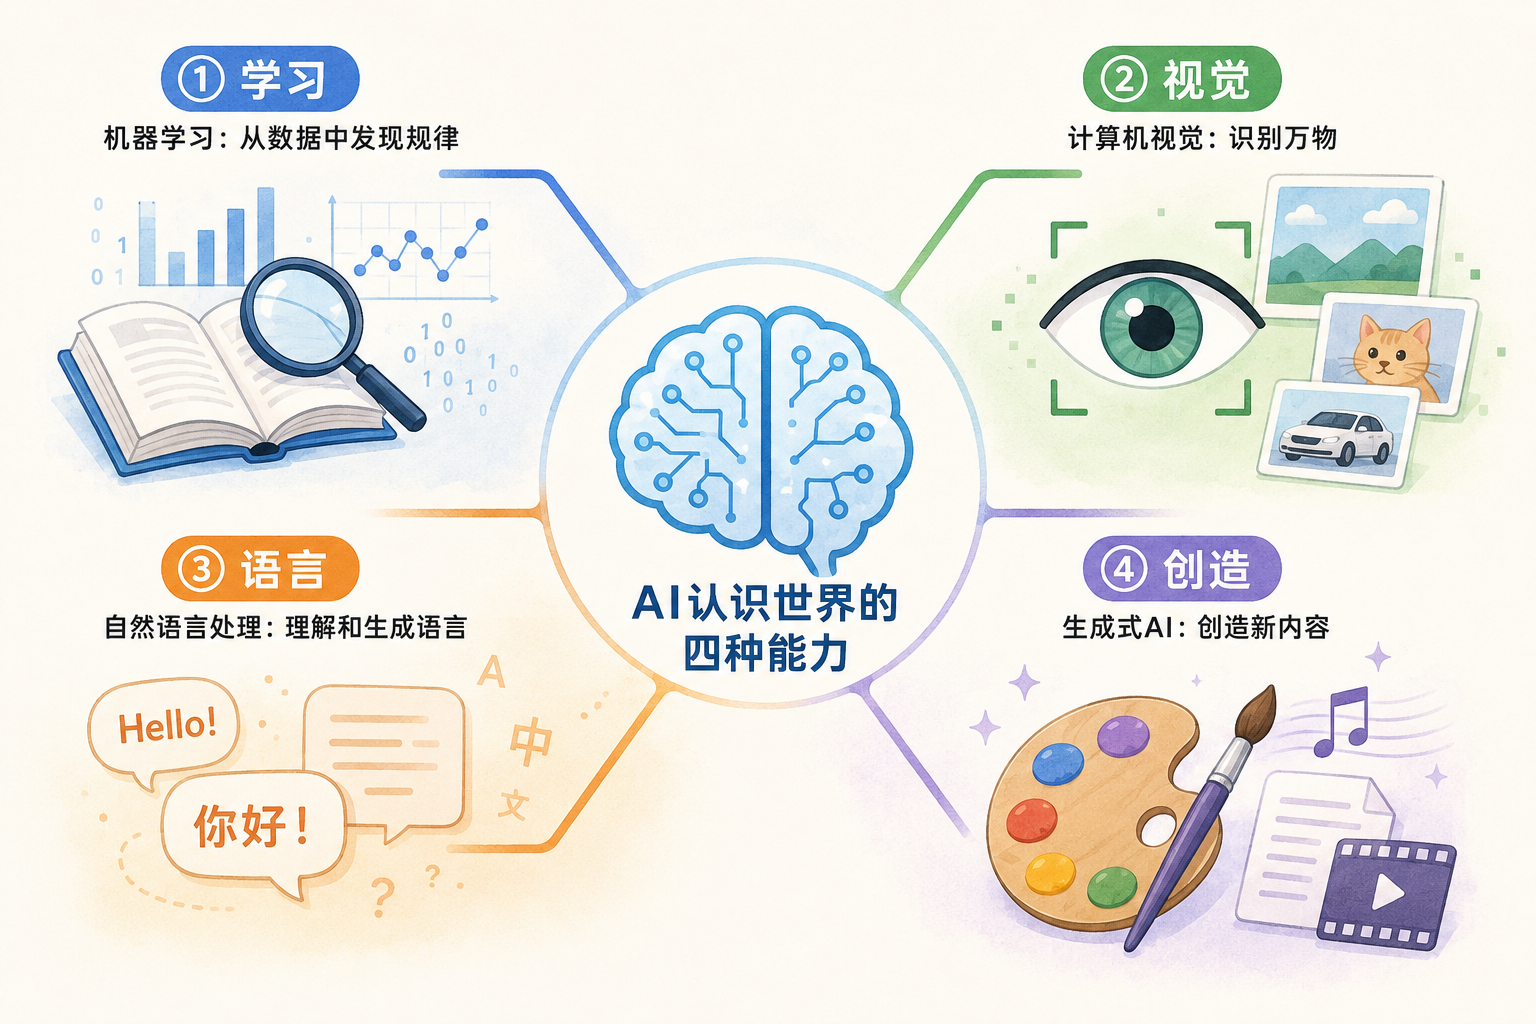
\includegraphics[width=0.88\textwidth]{./images_chapter_01-03/2.1.png}
\caption*{\footnotesize\itshape\color{gray!50} 图2-1\quad AI认识世界的四种能力——学习、视觉、语言、创造}
\end{figure}

\begin{center}
\color{gray!70} *\ \ *\ \ *
\end{center}
\vspace{12pt}

\section*{本章导览：AI的四项核心能力与一个共同边界}
\addcontentsline{toc}{section}{本章导览：AI的四项核心能力与一个共同边界}

在第一章中，我们站在生活体验的视角，看到了AI已经走进日常生活的方方面面——从短视频推荐到人机对话，从医疗影像到工厂质检。你可能还记得第一章中的几个关键结论：AI的本质是基于数据学习的预测系统，不是拥有自我意识的电子生命；AI的强大来自数据规模和算法精巧的结合；在绝大多数场景中，AI最恰当的角色是“增强人类”而非“替代人类”。

这一章，我们将把镜头推进到AI的“能力内部”。第一章中出现的那些令人印象深刻的案例——手机为什么能猜中你的喜好、人脸识别为什么有时会失败、大模型为什么能像人一样聊天、AI画画写文章到底靠不靠谱——它们的答案，都藏在AI的四项核心能力之中。

\textbf{机器学习}是AI的底层基础。它回答的是“AI到底是怎么从数据中学到东西的”这个根本问题。没有机器学习，后面要讲的视觉、语言、创造全都无从谈起。

\textbf{计算机视觉}是AI的“眼睛”。它让机器能从照片中认出人脸、从CT片中找出病灶、从马路上识别行人和车辆。

\textbf{自然语言处理}是AI的“语言大脑”。它让机器能翻译、能聊天、能总结论文、能写代码。第一章中让你震惊的ChatGPT，就是这项能力的最新代表。

\textbf{生成式AI}是AI的“创造之手”。它让机器能画画、写文章、做音乐、生成视频。第一章中提到的Midjourney获奖风波和Sora震撼发布，都源于这项能力。

在逐一展开这四项能力之后，我们将用最后一节来收束：\textbf{AI的边界与风险}。AI会“一本正经地胡说八道”吗？它会“戴有色眼镜”吗？它真正缺少的是什么？这些问题，是建立完整AI素养不可或缺的一部分。

在正式开始之前，有一个贯穿全章的核心概念想请你先记住。这个词叫\textbf{模式识别}——从数据中自动发现规律和特征的能力。它是贯穿机器学习、计算机视觉、自然语言处理和生成式AI的共同主线。无论是识别一张照片里的猫、拦截一条诈骗短信、还是一步步写出完整的剧情推理——AI做这些事情的基础，都是它在海量数据中找到了某种“模式”。理解了模式识别，你就拿到了理解AI所有能力的钥匙。

\begin{knowledgebox}
\textbf{模式识别——在数据中寻找隐藏的规律}

你观察到一个同学每天中午都去同一家面馆，久而久之，你就知道“明天中午去那家面馆大概率能碰到他”。你不需要知道他为什么喜欢吃面，也不需要了解他对碳水化合物的情感依赖，你只需要识别出“中午+这个同学=面馆”这个模式。这就是\textbf{模式识别}——从大量信息中自动发现重复出现的规律或特征，并用来预测未知。AI做的正是这件事：它同时观察着几亿人的成千上万种行为，发现着人类自己根本注意不到的模式。无论是机器学习、计算机视觉还是自然语言处理，AI做的归根结底都是同一件事：在海量数据中找到重复出现的规律，然后用来预测未知。
\end{knowledgebox}

让我们从那个最根本的问题开始：AI到底是怎么“学”的？

\section{机器学习：从数据中发现规律}

2016年3月，韩国首尔，围棋世界冠军李世石坐在棋盘前。对面不是人类，而是一台显示器。显示器那头，是DeepMind公司开发的AI——AlphaGo。比赛进行到第二局第37手，AlphaGo下出了一步棋。现场评论员一度以为系统出了故障——那步棋的位置，按照人类几千年围棋经验来看，“不合理”。

但AlphaGo不是人。它下那步棋，依据的不是人类总结的围棋定式，而是通过数百万局自我对弈自己发现的棋路。那手被称为“神之一手”的落子，后来被反复研究，被公认为极富战略远见。那一刻，全世界都看到了：AI不是在执行人类的智慧，而是在创造属于自己的——一种人类几千年围棋历史上从未出现过的、完全陌生的下法。

\begin{funbox}
\textbf{AlphaGo的“神之一手”——让围棋界震撼的一步棋}

2016年3月10日，韩国首尔四季酒店。世界围棋冠军李世石坐在棋盘前，对面是一台显示器的屏幕。这是他与AlphaGo五番棋对决的第二局。前一天，李世石已经输掉了第一局，但他仍然信心满满。

比赛进行到第37手。AlphaGo执黑，在棋盘右上角下了一步棋——黑子落在了五路。这步棋的位置让现场评论员一度以为系统出了故障。按照人类几千年围棋经验，这个位置“不合理”——它既没有直接抢占实地，也没有对白棋形成紧迫的威胁，看起来像是一步没有意义的“闲棋”。

但正是这步“闲棋”，在之后的数十手棋中逐渐展现了惊人的战略远见。它像一颗深埋的种子，在棋局发展到中盘时突然“开花”——这一步棋恰好策应了中腹的激战，让李世石陷入了攻守两难的境地。

“我从没见过人类下出这样的棋。”赛后，一位职业九段棋手如此评价。这手被称为“神之一手”的落子，不仅是AlphaGo战胜李世石的关键，更向全世界宣告：AI可以不依赖人类经验，通过自我学习发现全新的、超越人类认知的策略。
\end{funbox}

AlphaGo背后的技术，就是\textbf{机器学习}。它是现代人工智能最核心、最基础的引擎。没有机器学习，AI就只是一堆执行固定规则的代码——能计算、能排序，但永远不会“自己学会”任何事情。

\begin{knowledgebox}
\textbf{机器学习——让计算机从经验中自我提升}

机器学习是一门让计算机从数据中自动发现规律并据此做出预测的技术。与传统的计算机程序不同——传统程序靠人工逐条编写规则（“如果A则B”），机器学习则让计算机自己从大量例子中找出规律。就像你通过刷题来掌握解题技巧，而不是死记硬背每一道题的答案。
\end{knowledgebox}

\subsection{你的每一次点击，都在“训练”AI}

周五晚上十点，大二学生小周靠在宿舍床上，习惯性地打开短视频软件。他随手点开了一条NBA球星集锦——不过是一天课程结束后的消遣，他甚至没有点赞。

但接下来几天，奇怪的事发生了。推荐页里铺天盖地全是篮球内容：球鞋测评、战术分析、街球集锦、NBA历史经典回顾……小周翻了半天，忍不住嘟囔：“我没搜索过啊，它怎么知道我喜欢篮球？”

他不是唯一有这种困惑的人。小周的同学阿琳发现，自己只是在购物软件里多看了几眼运动鞋，首页就变成了运动装备专场。另一位同学在朋友圈吐槽：“我就在搜索框里打了一次‘考研’，现在整个App都在给我推‘上岸经验’，甚至开始推防脱洗发水了。”

不只是娱乐和购物。你的手机输入法似乎知道你接下来想打什么字。外卖软件记得你喜欢“少盐”“不要香菜”。音乐App总能推给你一听就上瘾的歌。地图导航知道你每天早上八点要去教学楼、下午五点要去食堂。

这些App当然没有在你身上装摄像头。它们唯一掌握的东西，是你留在它们那里的\textbf{行为数据}——你看了什么、停了多久、点了什么、搜了哪个关键词。把这些零散的行为碎片拼在一起，就形成了一幅关于你的越来越精准的画像。

\begin{figure}[H]
\centering
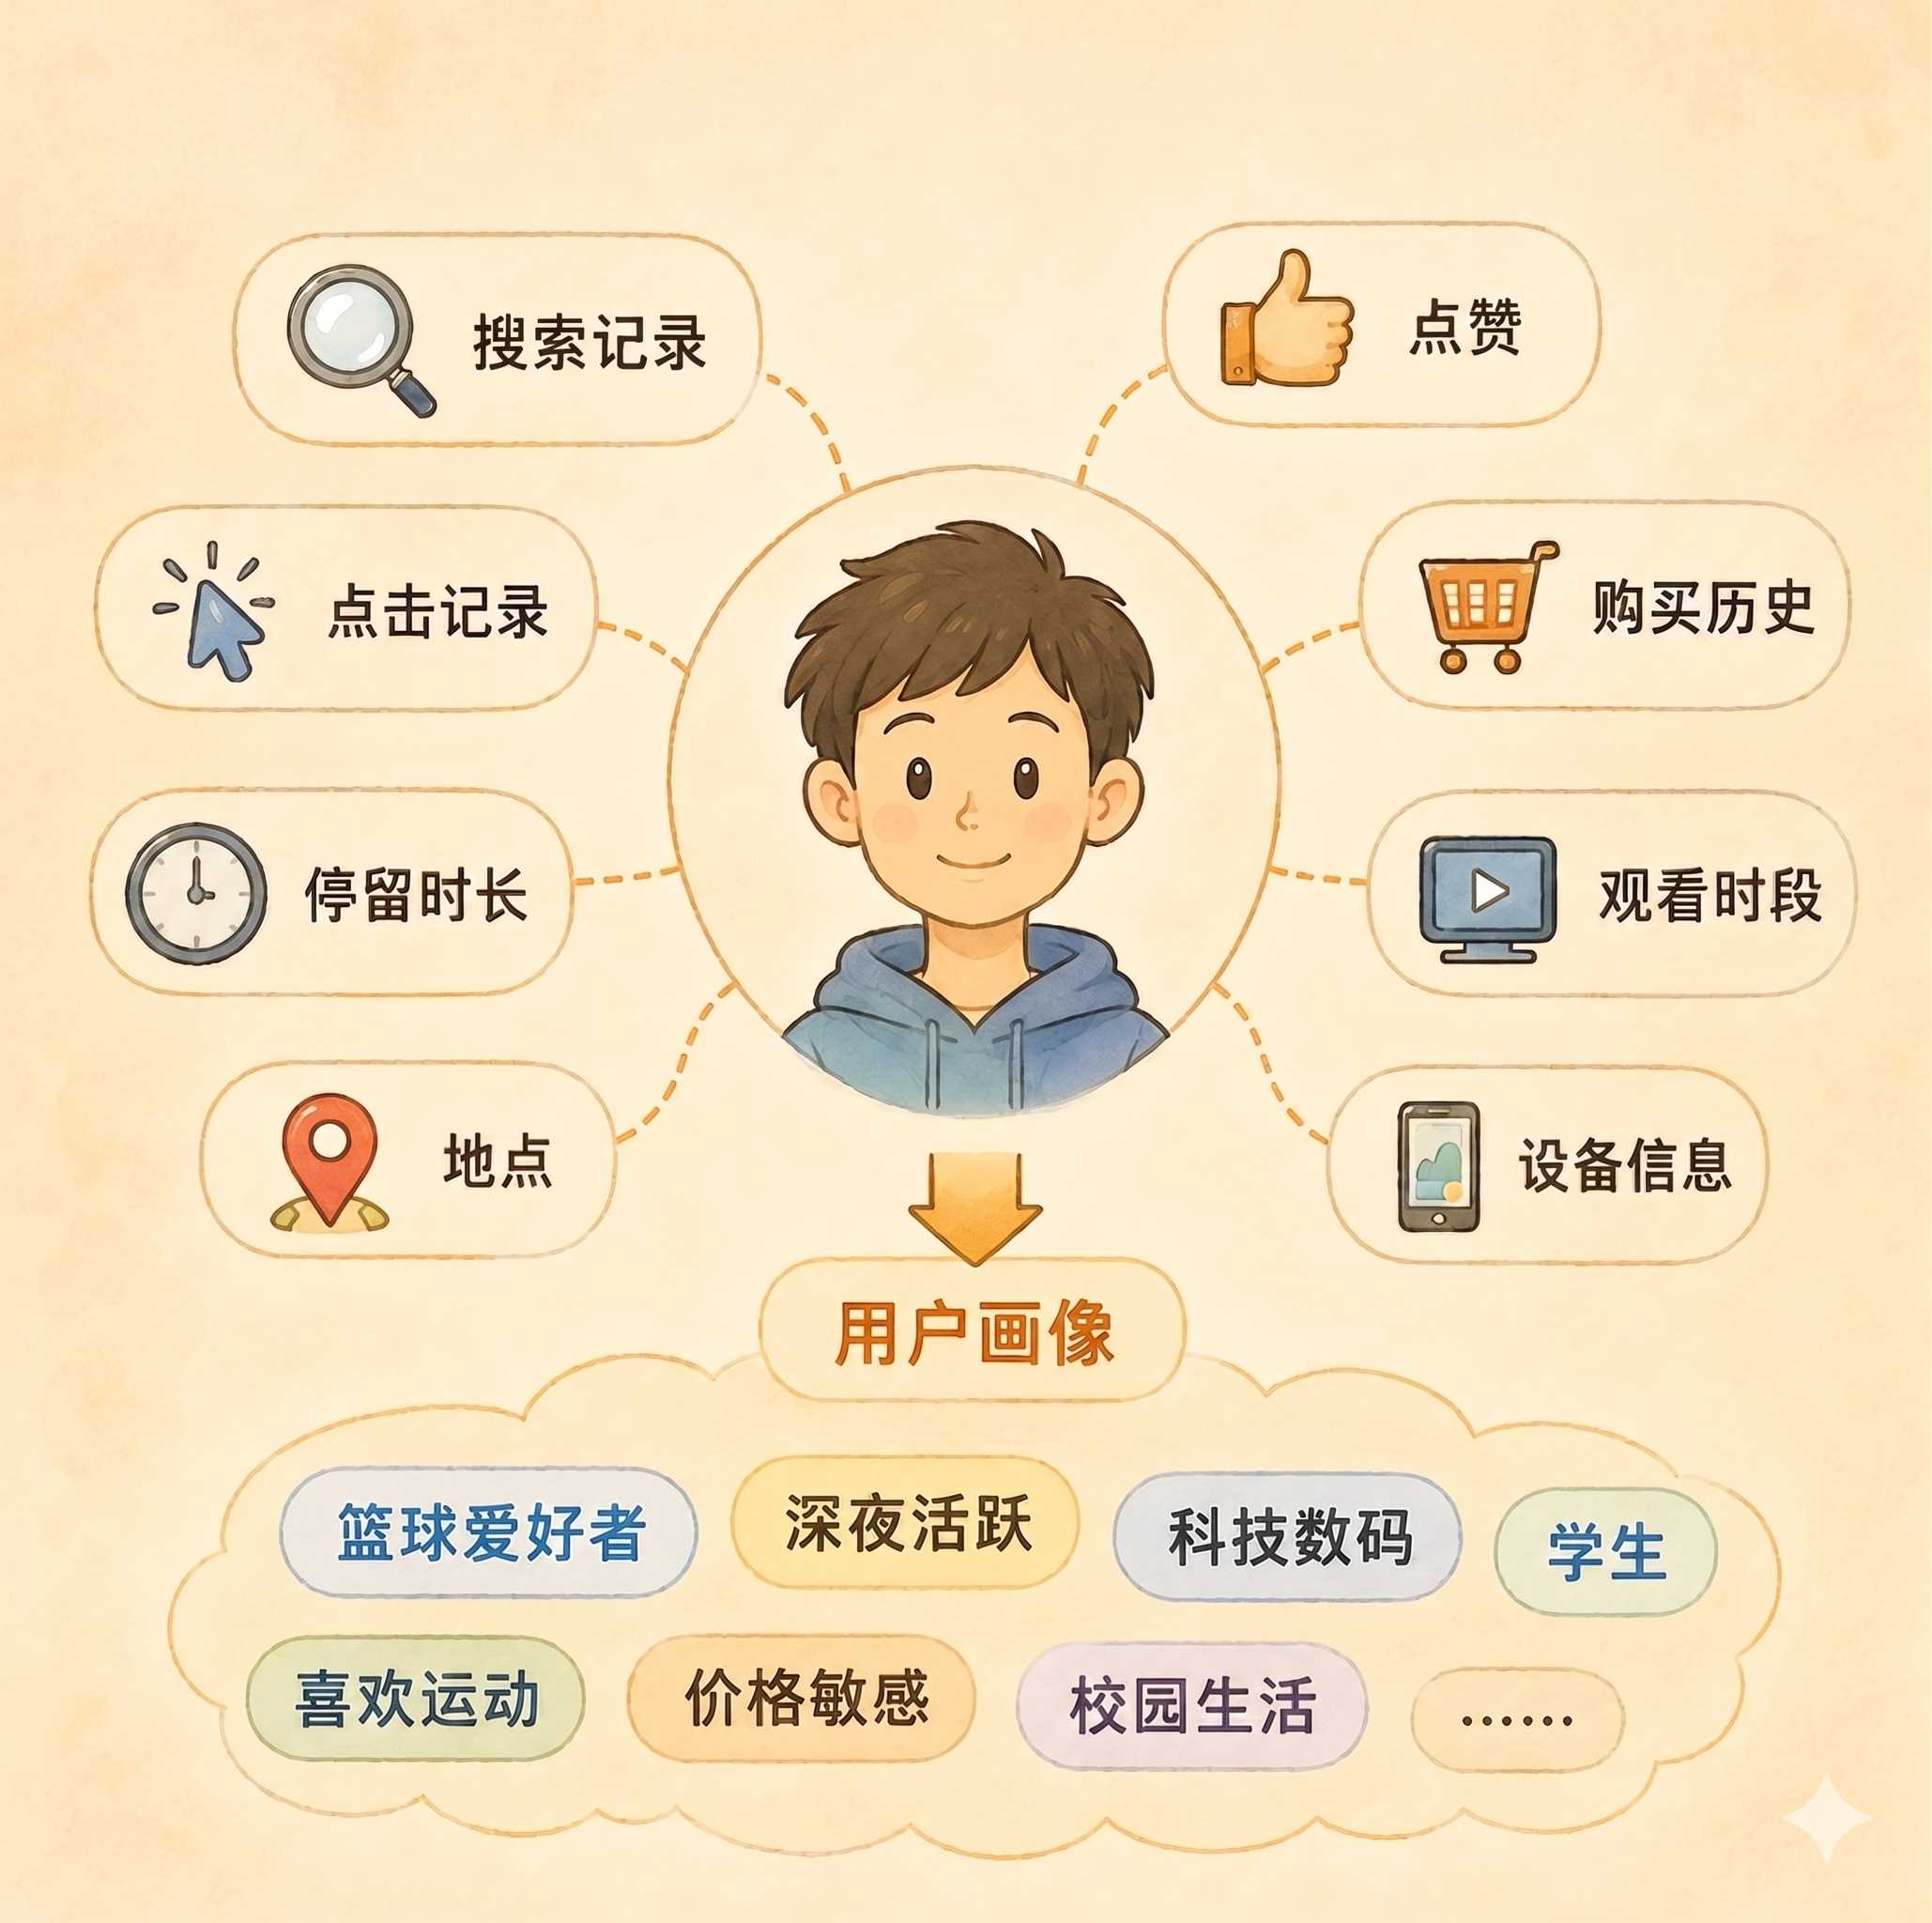
\includegraphics[width=0.88\textwidth]{images_chapter_01-03/2-2.png}
\caption*{\footnotesize\itshape\color{gray!50} 图2-2\quad 推荐系统如何从行为数据中“拼出”用户画像}
\end{figure}

这些行为数据是如何被AI使用的？平台记录的不是“小周喜欢篮球”，而是更具体、更原始的数据：他在某个视频上停留了3分28秒（全长3分30秒），看完后又手动回拖到第45秒重看了一遍慢动作回放。他点赞了三段类似视频中的两段，划走了另一段——因为那段是足球。

对于AI来说，这些行为组合在一起，几乎等于小周在大声喊：“我对篮球非常感兴趣！”

\textbf{一个有趣的真相：你其实是“免费的数据标注员”}

2016年，谷歌推出过一个叫“Quick, Draw!”的小游戏。规则很简单：你需要在20秒内画出一个指定物体（比如自行车、房子、长颈鹿），AI需要在20秒内猜出你画的是什么。这个游戏看起来可爱无害，但它帮谷歌收集了超过5000万张手绘涂鸦。这些涂鸦后来被用来训练AI理解人类如何画画——不是从照片中识别物体，而是从歪歪扭扭的简笔画中理解人类的表达方式。

你和朋友们在玩这个游戏的时候，其实是在免费帮谷歌训练AI。同样，你每一次点赞、每一次停留、每一次滑动屏幕，都在“告诉”AI：这个我喜欢，那个我没兴趣。你不是在“被AI观察”，你是在“帮AI变得更了解你”。

那么问题来了：这些看似零碎的行为碎片，到底是怎么被拼成一幅关于“你”的完整画像的？AI到底从这些数据中“学”到了什么？

\subsection{手机为什么总能“猜中”你的喜好}

让我们继续追踪小周的故事。

小周仔细回忆了自己这几天的行为：他没有搜索过“篮球”，没有关注篮球博主，也没有在篮球视频下留言。他做的唯一一件事，是那条NBA集锦视频他完整看完了，还反复看了几遍。

就凭这个？是的，就凭这个。

这里有一个很多人没意识到的关键：\textbf{“看了什么”比“说了什么”更重要。} 我们的嘴巴会说谎（“我要好好学习”），但手指很诚实——它诚实地在萌宠视频上停留了四十分钟。

平台收集到用户行为数据后，会进行一系列处理。不是某一条数据单独起作用，而是多种行为数据综合在一起形成判断。你看了什么内容、停留了多久、有没有点开评论区、看完整内容还是中途划走、看完之后有没有搜索相关内容、在什么时间段打开App——每一条单独看都说明不了什么，但组合在一起就极有信息量。AI不用理解“喜欢”这种情感是什么，它只需要知道：当“观看完成率超过95\%”和“主动回拖重看”和“接下来几天持续打开App”这三个行为同时出现时，把同类内容推到用户面前几乎一定是对的。

“用户画像”这个概念听起来很新，但它的底层逻辑其实比互联网还要古老。早在1940年代，美国社会学家就在做类似的事——通过分析人们的年龄、职业、居住地，来预测人们会买什么东西、投给哪个政客。只不过那时候靠的是问卷调查和人口统计，现在靠的是你手指的每一次滑动。

AI的“猜你喜欢”，本质和百货商场把化妆品放在一楼、把男装放在三楼是同一个逻辑：通过观察大量人的行为，总结出规律，然后预测下一个人的需求。AI唯一的不同是它能观察的人数远超任何一个人类——它能同时“记住”几亿人的所有行为，并从中找到人类根本无法靠手工发现的关联。

既然AI这么擅长发现规律，那它具体是怎么“学”的？这就要讲到现代人工智能最核心的技术——\textbf{机器学习}。

\subsection{机器学习——像教小孩一样教AI}

如果你要教一个两岁的小孩认识猫，你会怎么做？你不会让他读《猫科动物解剖学》，也不会给他讲“猫属于哺乳纲食肉目猫科”。你只会不断给他看猫的图片、带他去看邻居家的猫、指着街上的猫说“猫咪”。一开始他可能会把狗也认成猫。没关系，你纠正几次：这个不是猫，是狗狗。那个也不是猫，是兔兔。慢慢地，他就学会了。

\textbf{机器学习的基本逻辑，和这个过程几乎一模一样。}

\begin{figure}[H]
\centering
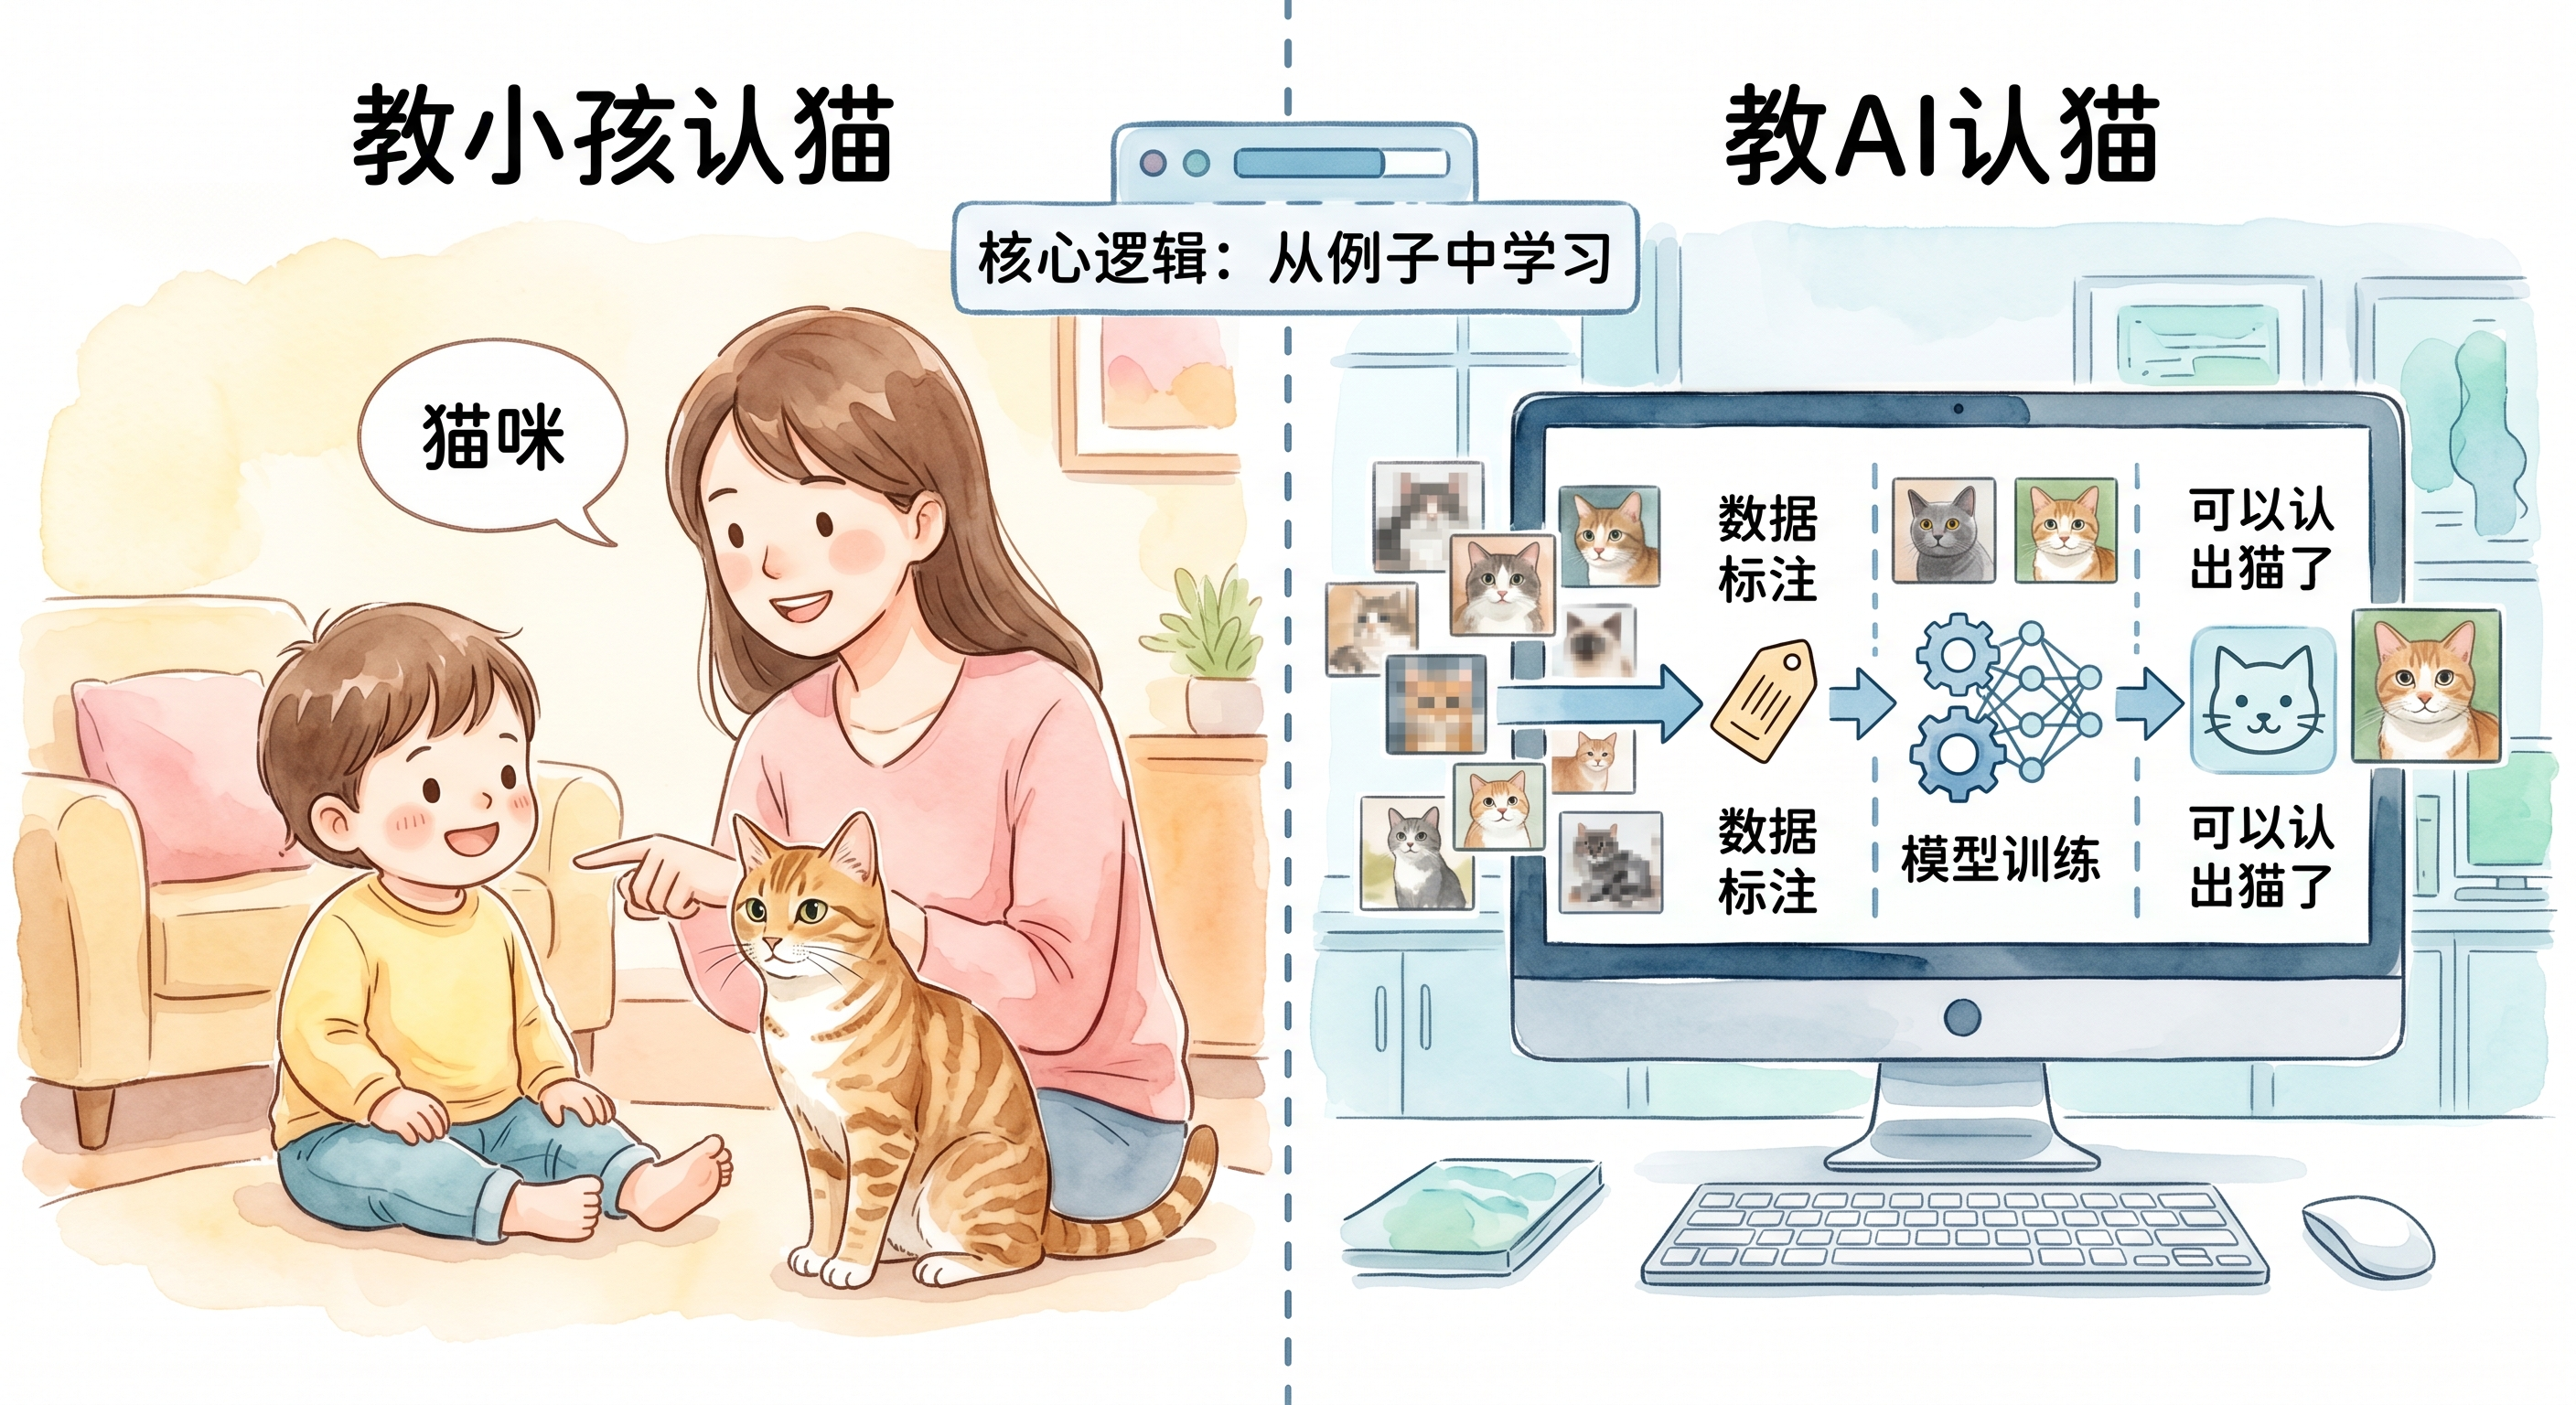
\includegraphics[width=0.88\textwidth]{images_chapter_01-03/2-3.png}
\caption*{\footnotesize\itshape\color{gray!50} 图2-3\quad 推荐系统如何从行为数据中“拼出”用户画像}
\end{figure}

传统的计算机程序，是靠人工编写规则来运行的。如果你想写一个“识别猫”的传统程序，你得一条条写规则：“如果这个动物有四条腿、尖耳朵、长胡须、会喵喵叫，那就是猫。”但问题来了——有些猫耳朵是垂下来的，有些猫胡须不明显，斯芬克斯无毛猫全身光溜溜的。规则永远写不完，例外永远存在。

机器学习换了一种思路：\textbf{不给AI写规则，给它看成千上万个例子，让它自己找规律。}

这个过程可以用学生最熟悉的场景来类比——刷题。你不会把每道题的标准答案背下来，数学题千变万化，你背不完。你是通过刷大量题目来总结“这类题应该怎么解”的规律。AI也一样。给它“投喂”海量标注好的数据——这叫\textbf{数据集}。AI从中提取特征、总结规律、不断修正错误，最终形成稳定的判断能力。这个过程叫\textbf{模型训练}。训练完成的AI就像一个刷了十万道题的学生，再遇到类似的问题，就能给出比较准确的判断。

\begin{figure}[H]
\centering
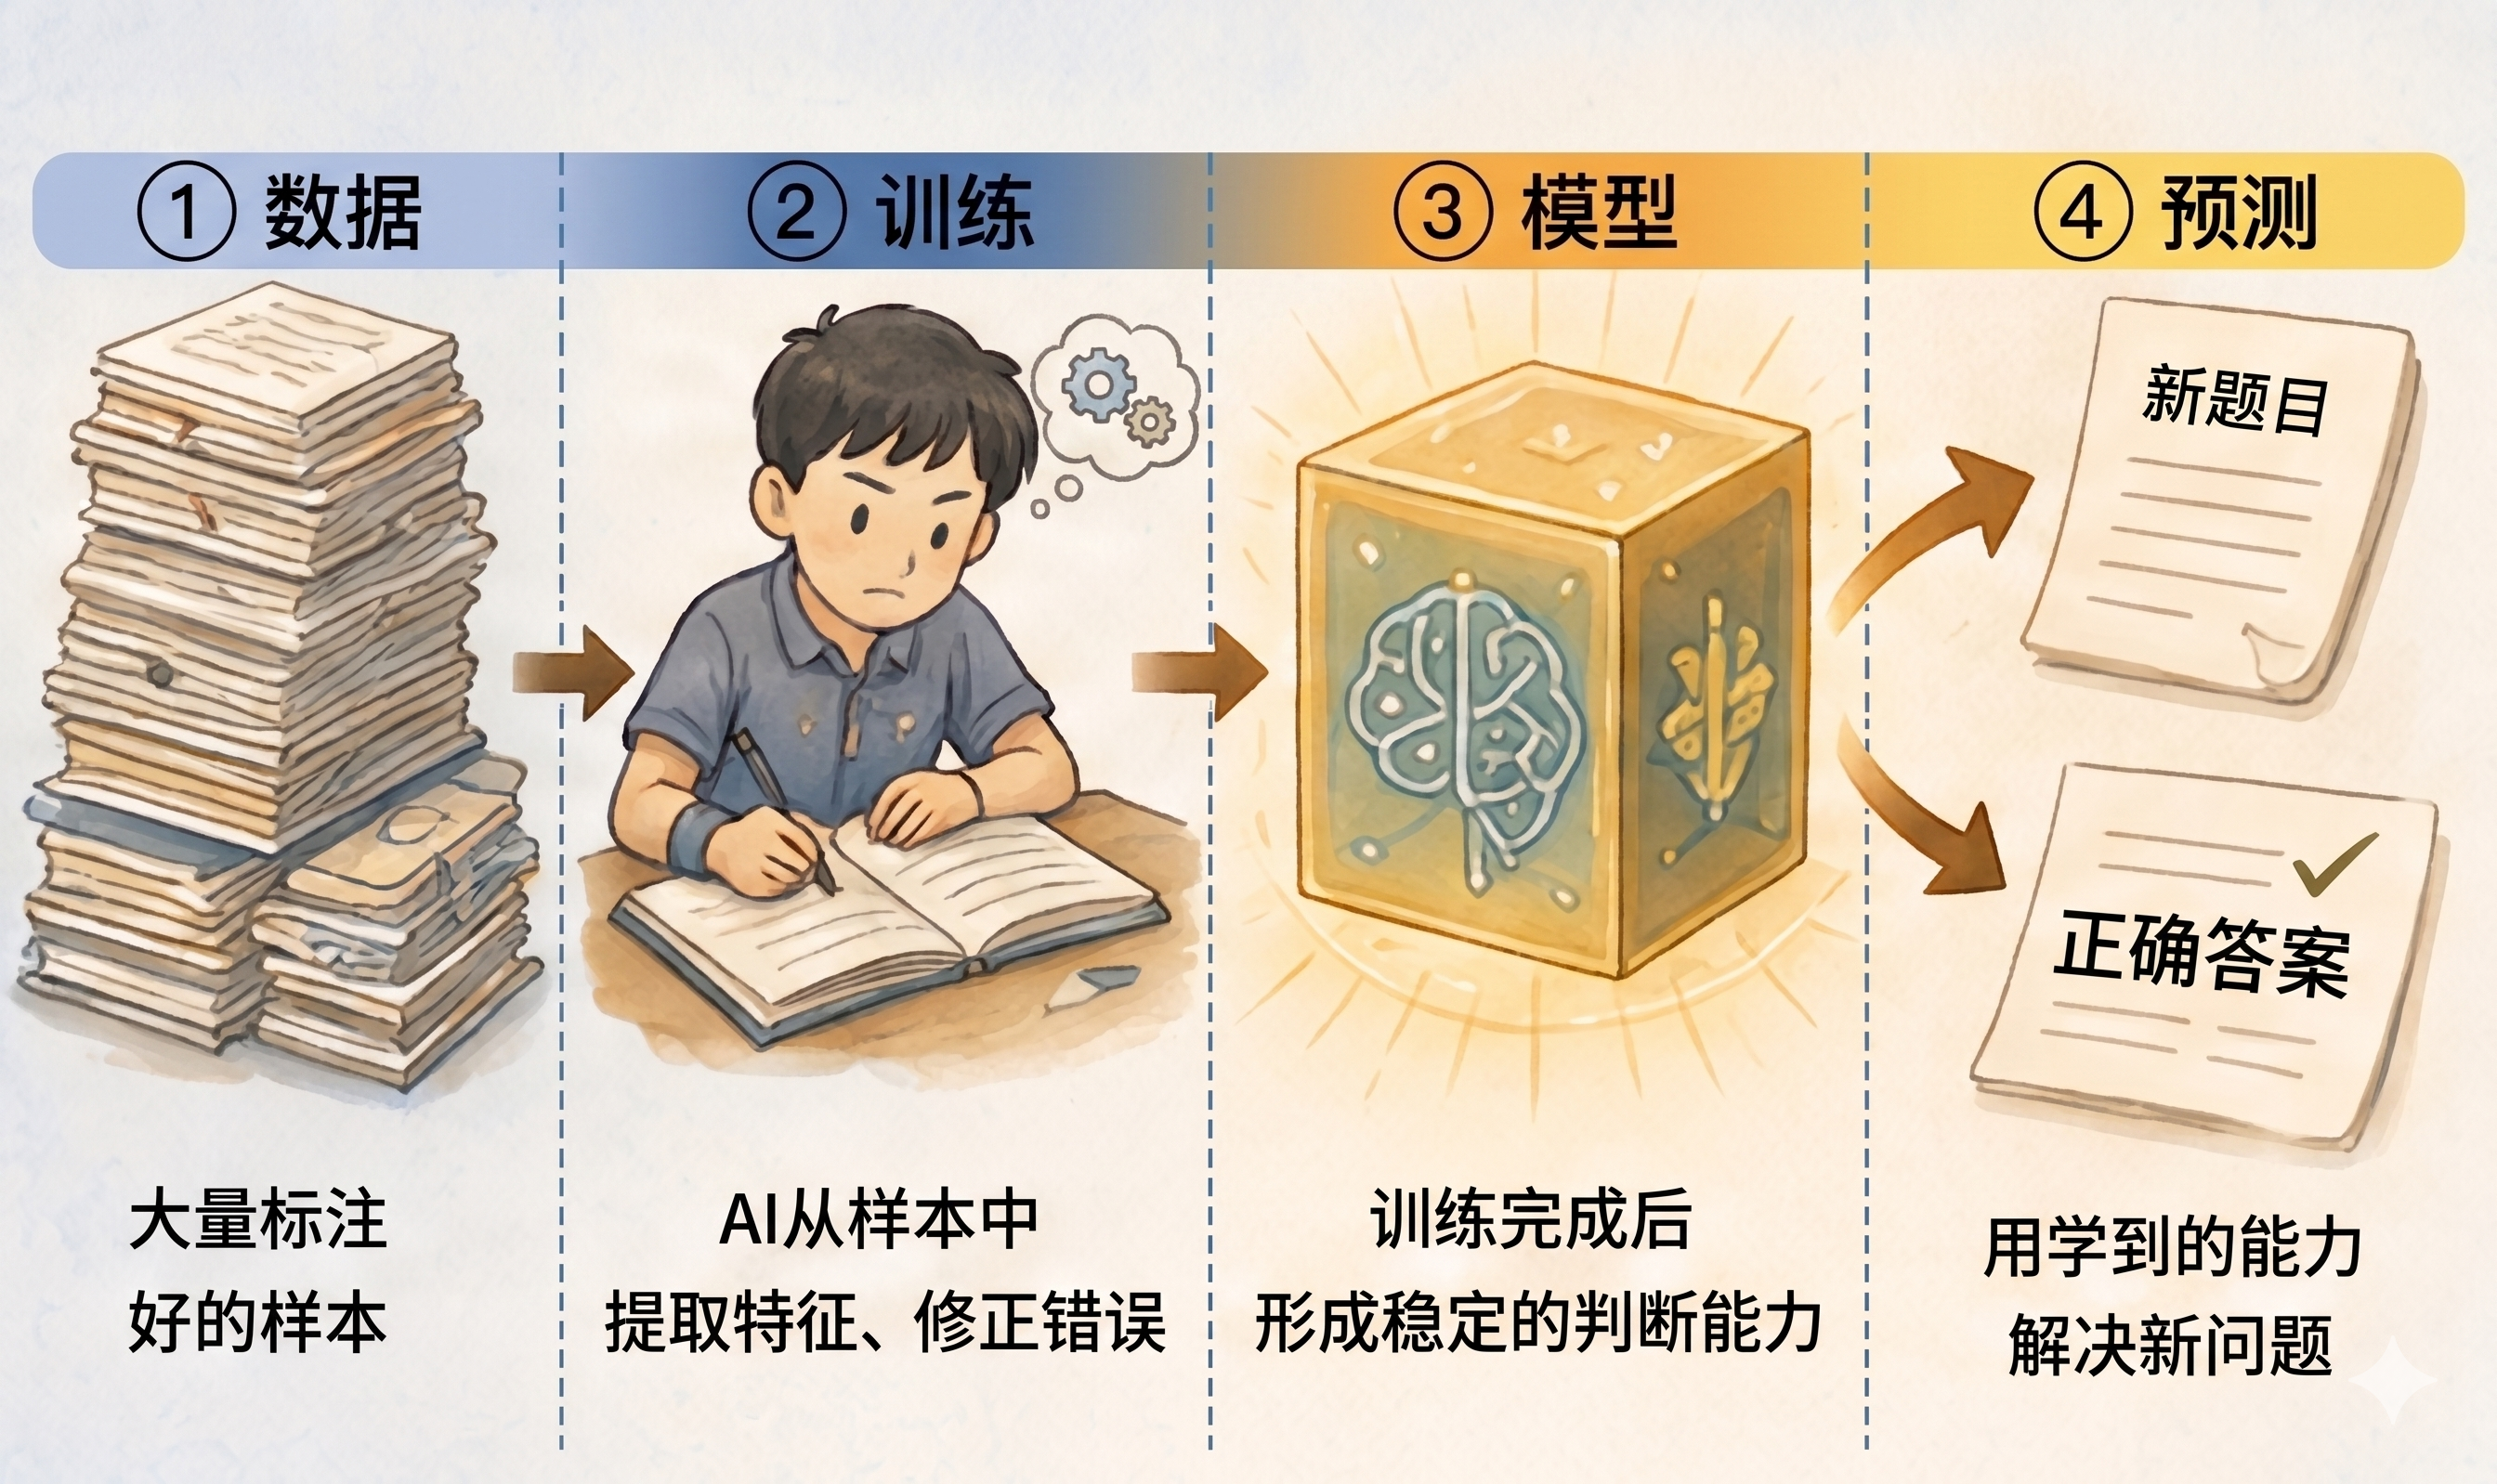
\includegraphics[width=0.88\textwidth]{images_chapter_01-03/2-4.png}
\caption*{\footnotesize\itshape\color{gray!50} 图2-4\quad 推荐系统如何从行为数据中“拼出”用户画像}
\end{figure}

这个过程中最关键的是什么？\textbf{数据。} AI的能力上限，很大程度上取决于“投喂”给它的数据质量。如果训练数据里猫的照片都是在白天拍的，AI在晚上可能就认不出猫了。如果数据里大多是橘猫，AI面对黑猫时可能会犹豫。如果数据本身带有偏见——比如“医生”的图片大多是男性——AI就会学到这个偏见并忠实地复制它。

\begin{knowledgebox}
\textbf{数据集与数据标注——AI的“教材”与“标准答案”}

想象你要教一个从没见过猫的外星人认识猫。最好的办法就是给它看几百张猫的照片，每张照片背面写上“这是猫”。这些照片就是\textbf{数据集}——用来训练AI的样本集合。照片背面的文字就是\textbf{数据标注}——给训练样本贴上正确答案的标签。标注通常由人工完成，非常耗时耗力。但标注质量直接决定AI学得好不好——标注错了，AI就会学错。AI领域因此流行一句玩笑话：“AI的智能，其实是被一群按件计酬的数据标注员‘喂’出来的。”
\end{knowledgebox}

机器学习是本章所有后续内容的基础。接下来你会看到，计算机视觉是机器学习在图像上的应用，自然语言处理是机器学习在文本上的应用，生成式AI是机器学习从“识别”向“创造”的进阶。它们共享同一个底层逻辑：\textbf{从数据中学习规律，然后用规律来预测未知。}

那么，机器学习到底能在现实生活中做什么？只是认猫认狗和推荐视频吗？

\begin{funbox}
\textbf{谷歌大脑的“猫脸”实验——AI自己“发现”了猫}

2012年，谷歌大脑（Google Brain）的研究者做了一个当时看来有些“疯狂”的实验。他们用16000个计算机处理器组成了一个庞大的神经网络，然后让它“看”了1000万张从YouTube视频中随机截取的图片。他们没有告诉AI任何关于这些图片的知识——没有标注“这是猫”“这是人脸”“这是一辆自行车”。他们只是让AI自己去看。

训练结束后，研究者检查了这个神经网络的内部状态。一个令人震惊的发现浮出水面：在这个完全自学、无人指导的过程中，AI自发地“进化”出了一个对“猫脸”高度敏感的神经元。它不知道“猫”这个词，没见过“猫科动物”的定义，但它从1000万张图片的统计规律中自己“发现”了：这种圆脸、尖耳朵、长胡须的物体在图片中反复出现，一定是某种重要的存在。

这个故事最迷人的地方在于：AI的学习方式，某种程度上与婴儿认识世界的方式有相似之处——不需要被告知“这是什么”，只需要看到足够多的例子，就能自己总结出规律。
\end{funbox}

\subsection{机器学习应用案例}

机器学习已经渗透到我们生活的各个角落。在学习领域，它帮你自动批改作文、推荐适合你水平的练习题；在安全领域，它识别诈骗短信和异常交易；在交通领域，它预测路况和优化导航路线；在气象领域，它分析卫星云图预测天气；在医学领域，它辅助医生发现早期病灶；在商业领域，它分析用户行为精准推荐商品。从你手机里的输入法到天上的气象卫星，从医院的CT机到电商平台的推荐引擎——机器学习的应用广度远超大多数人的想象。

下面，我们通过三个具体案例，看看这项技术是如何在不同领域真实运作的。

\subsubsection*{案例1：诈骗短信为什么会被自动拦截}

晚上十一点，大一学生小李的手机突然震了一下。他迷迷糊糊拿起手机，屏幕上的短信预览让他瞬间清醒：“【快递通知】您的包裹因地址填写错误已被退回，请立即点击链接重新确认，否则24小时后将自动销毁。”短信里快递公司的名称、客服电话、页面格式，都和真的一模一样。小李确实有两个快递在路上，他手指已经悬在了链接上方。

就在这时，手机顶部弹出一行灰色小字：“⚠️ 疑似诈骗短信，已被系统自动拦截至垃圾箱。”

小李长舒一口气。但他随即产生了一个疑问：机器到底是怎么知道这是一条诈骗短信的？

它并不像人类一样“看懂”了这条短信的内容。它不知道什么叫“欺骗”，什么叫“利用人的焦虑心理”。它只是在海量历史数据中，寻找诈骗短信的共同模式。当被举报过的诈骗短信积累到百万级、千万级时，某些规律就自然浮现了：诈骗短信里大量出现“包裹退回”“地址错误”“立即点击”“自动销毁”这类制造紧迫感的关键词组合；链接通常是不明短链接或仿冒域名；发送号码往往是虚拟号段或境外号码；发送行为也很特别——短时间内大规模群发，不像普通人发短信的节奏。

正常短信完全不是这个画风：快递通知告知取件码和驿站地址，语气平稳；银行短信包含具体金额和卡号尾号，不会让你点不明链接。

AI通过对比海量的“诈骗短信”和“正常短信”，逐渐学会了一套判断规则。它做的其实是一个概率计算：“综合来看，这条短信像诈骗短信的概率有多高？”当概率超过99\%时，直接拦截；当概率在60\%左右时，标记为“疑似”放进垃圾箱，等你手动确认。

这个案例的核心启示是：AI并不“懂诈骗”，它只是在做模式识别——从海量数据中总结重复出现的规律。而这，正是机器学习最核心的能力。

\begin{figure}[H]
\centering
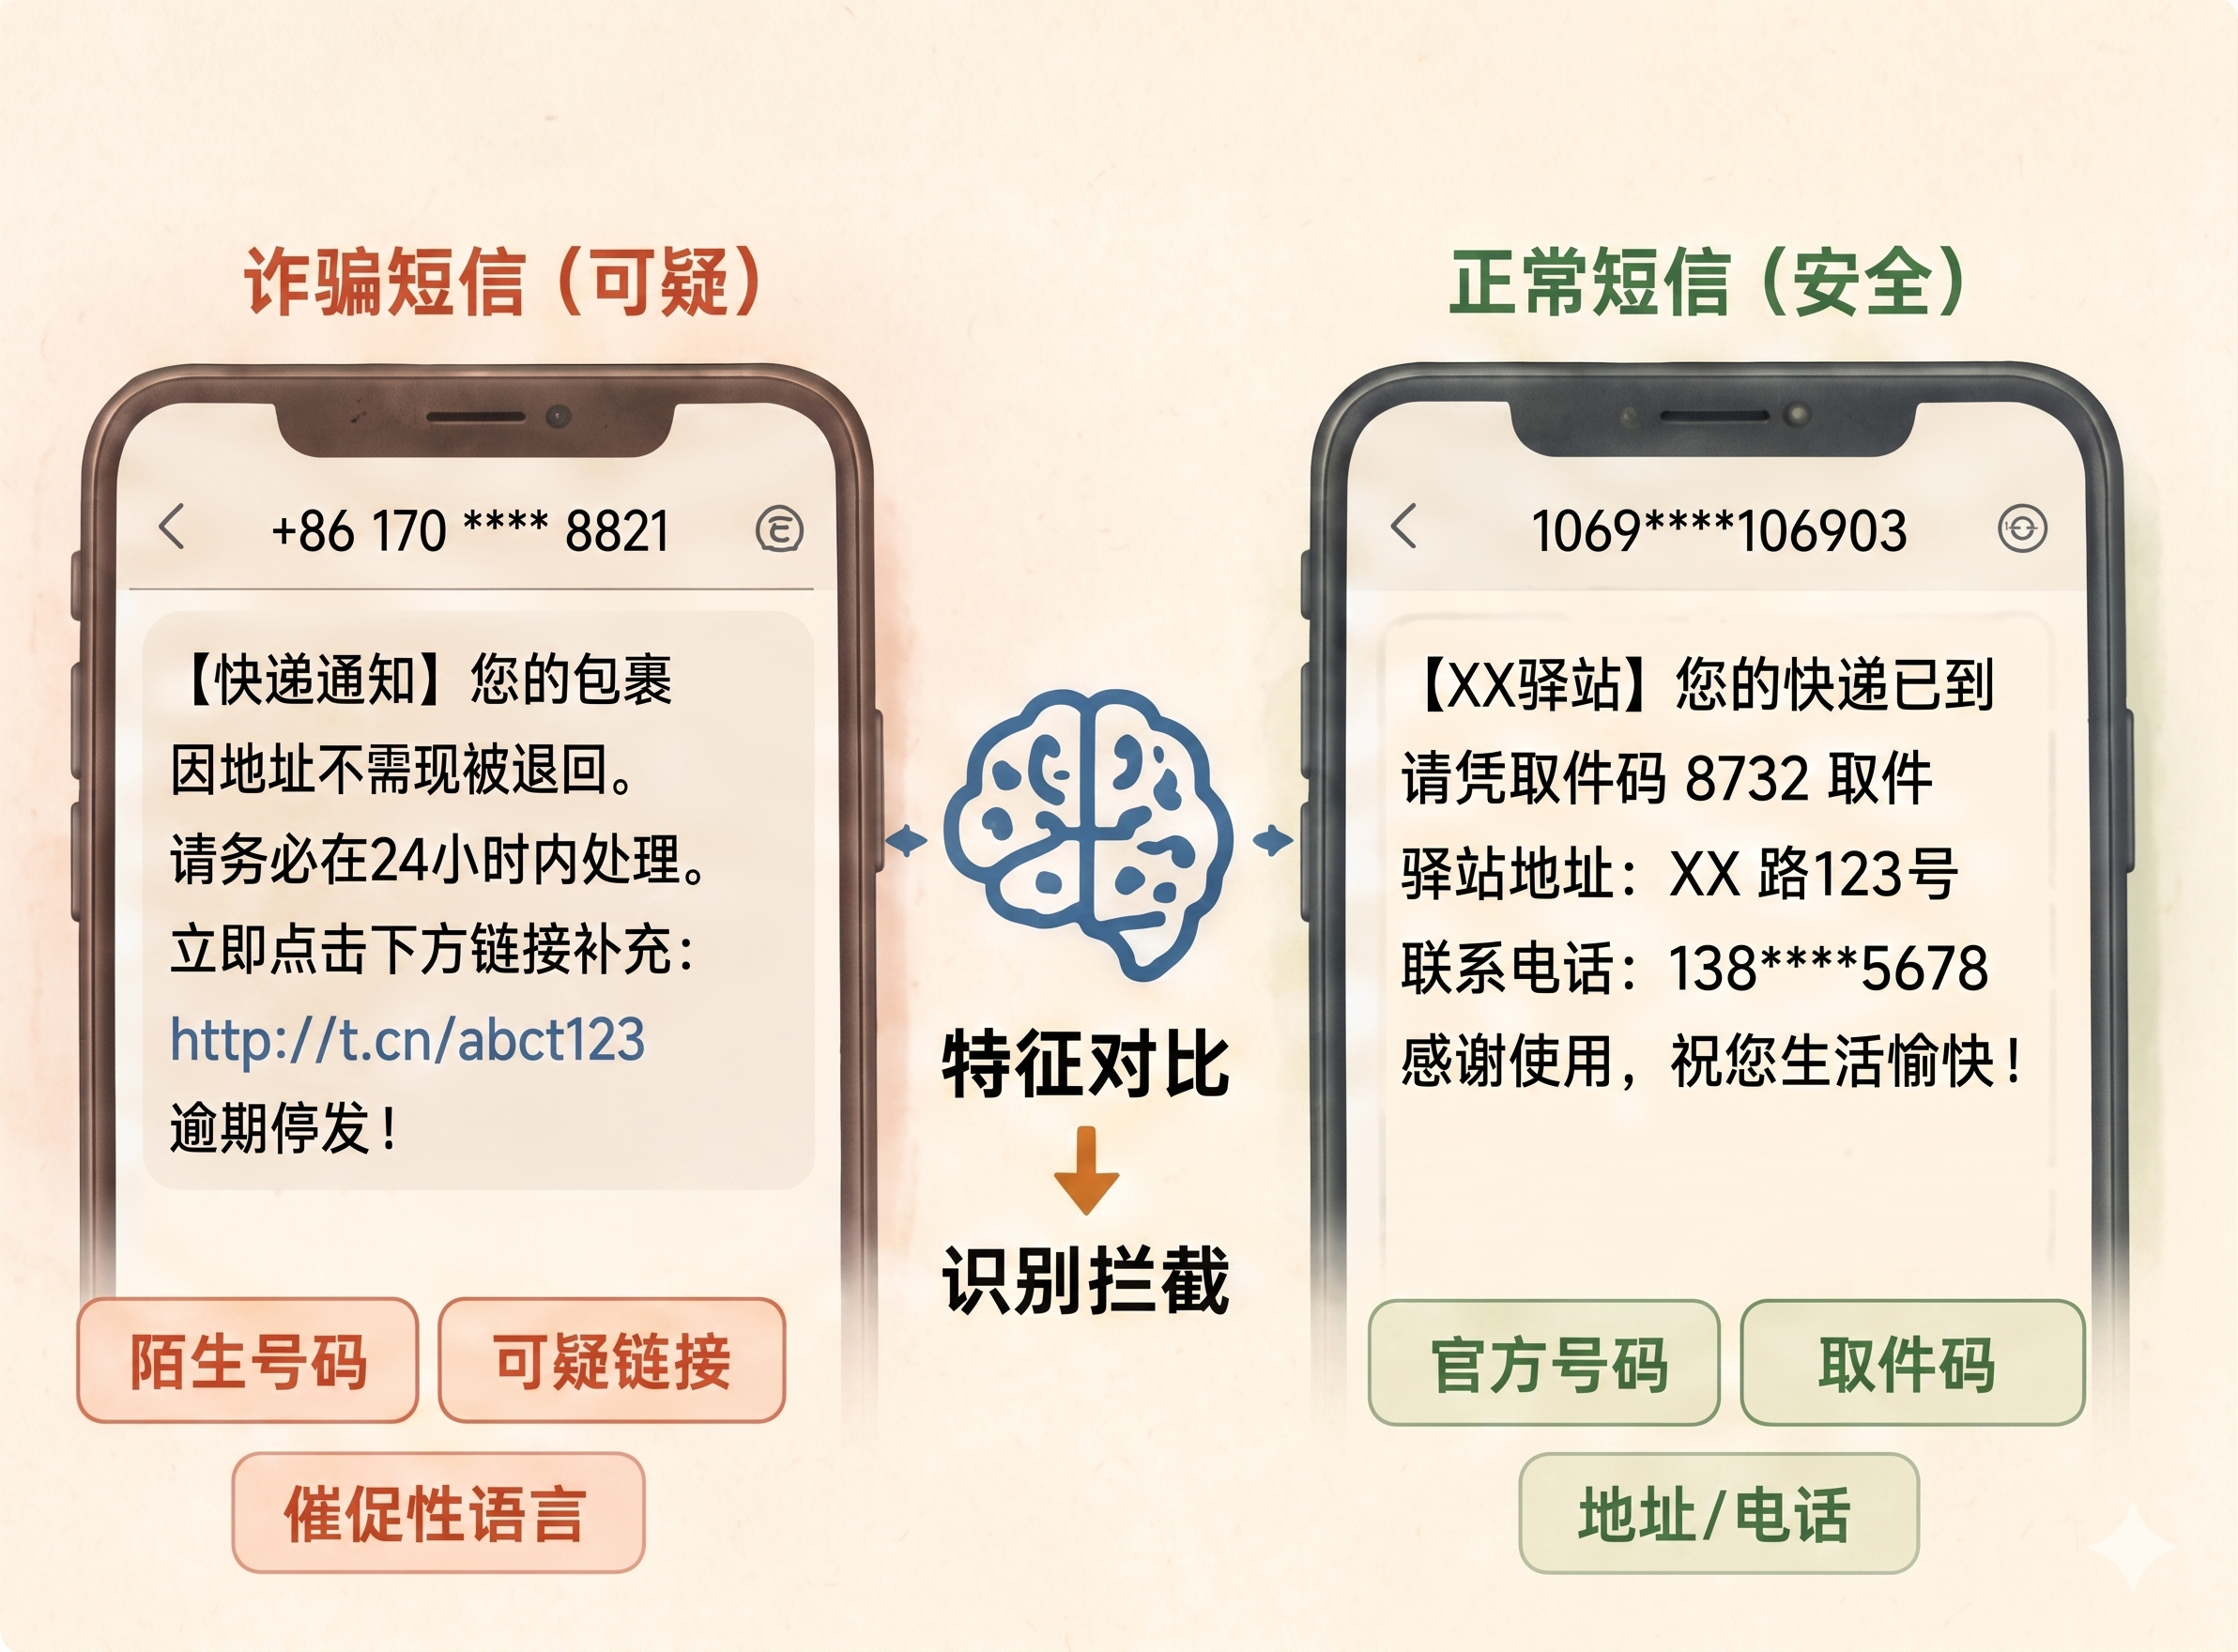
\includegraphics[width=0.88\textwidth]{images_chapter_01-03/2-4b.png}
\caption*{\footnotesize\itshape\color{gray!50} 图2-4b\quad 推荐系统如何从行为数据中“拼出”用户画像}
\end{figure}

\subsubsection*{案例2：输入法是怎么“猜”到你要打的字}

你每天都在用输入法打字，但你可能注意过这样一个细节：当你打出“我今天想去”这几个字后，输入法会自动在候选栏里推荐“学校”“食堂”“图书馆”“超市”这些词。它怎么知道你想说什么？

输入法背后的AI系统，通过分析海量用户的打字数据来学习语言规律。它记录的不是“某个具体的人在打什么字”，而是“某个词后面最常跟着什么词”。比如“想去”这个词，在海量数据中后面跟着“学校”的概率是15\%，跟着“食堂”的概率是12\%，跟着“图书馆”的概率是8\%。当你打出“我今天想去”时，AI就根据这个统计规律，把最可能的后接词推送到候选栏的前排。

更有趣的是，输入法还能学习你个人的打字习惯。如果你是一个经常打“我想去打篮球”的人，AI就会在你的个人模型里把“篮球”的权重调高。下次你再打“我想去”，它会在候选栏更靠前的位置显示“打篮球”。这就是为什么用同一款输入法的人，推荐的词却各不相同——AI已经悄悄“摸透”了你的表达习惯。

这个案例的核心启示是：AI不“懂”语言，它只是通过海量数据中的词频统计和搭配规律，计算出最可能的下一个词。你每一次打字，都在帮AI变得更“了解”你的表达方式。

\begin{knowledgebox}
\textbf{语言模型——AI的“词语接龙”高手}

输入法背后使用的技术，在AI领域被称为\textbf{语言模型}。你可以把它想象成一个玩“词语接龙”的超级高手。它读遍了人类写过的几乎所有文本，记住了“高兴”后面常跟着“快乐”，“天气”后面常跟着“晴朗”。当你输入“今天天气”，它的大脑（其实是一个巨大的概率表）立刻浮现出“真好”“晴朗”“糟糕”等选项，并挑出最可能的那一个推荐给你。它不知道这些词的意思，但比任何人都更熟悉它们之间的搭配关系。
\end{knowledgebox}

\subsubsection*{案例3：AI如何预测天气}

“明天局部地区有雨”——这句天气预报的背后，是AI对海量气象数据的分析。

气象卫星每天从地球各个角落传回温度、湿度、气压、风速、云层厚度等数据，数据量以TB计。人类预报员不可能在短时间内处理完这么多信息。而机器学习模型可以——它“吃”进过去几十年的历史气象数据，从中学习天气变化的规律：某个区域的气压下降3百帕通常意味着什么？海洋表面温度升高1度会对台风路径产生什么影响？各种气象要素之间有什么复杂的非线性关系？

通过这些学习，AI能对未来几小时到未来两周的天气做出预测。虽然天气预报偶尔还是不准——因为天气系统是极端复杂的混沌系统，微小变化都可能引发巨大的预测偏差——但相比几十年前纯靠人工经验和简单物理模型的时代，AI让预报准确率大大提升。今天，AI甚至可以预测某个具体位置的“未来两小时降雨量”——精确到分钟级和百米级，帮你决定“现在出门要不要带伞”。

这个案例的核心启示是：机器学习的本质，是让AI从历史数据中总结规律，然后用这些规律来预判未知事件。从拦截诈骗短信到预测天气，从猜你想打的字到辅助诊断疾病，这项技术已经渗透到生活的方方面面。

\begin{knowledgebox}
\textbf{混沌系统——一只蝴蝶引发龙卷风}

天气预报之所以偶尔失灵，根子在于天气是一个典型的\textbf{混沌系统}。混沌系统最著名的比喻是“蝴蝶效应”：一只蝴蝶在巴西扇动翅膀，可能引发德克萨斯的一场龙卷风。因为系统对初始条件极其敏感，任何微小的测量误差，都会在预测中被迅速放大。所以，天气预报达不到100\%准确，这不是AI的错，而是天气本身那难以捉摸的本性。
\end{knowledgebox}

\subsection{AI真的会“思考”吗}

先讲一个有点好笑的真实经历。小周买过一双篮球鞋。买完之后，他连续三天都在购物App的首页看到更多篮球鞋推荐——不同品牌、不同配色、不同价位，全都是篮球鞋。问题在于：\textbf{他已经买过了。}

一个正常人类店员不会在你刚刚买了一双鞋走出店门后追出来喊：“先生先生！您可能还对这双鞋感兴趣！”但AI会。因为它并不理解“买过了”和“还没买”的区别。它只知道你最近对篮球鞋表现出很强的兴趣——非常强——所以继续推荐。

这就是AI的第一个局限：\textbf{没有常识。} AI知道的是数据告诉它的东西：你看了篮球鞋，篮球鞋和运动相关，所以推更多篮球鞋。但它不理解“人一般不会短时间内买两双同类型的鞋”这个常识。

如果你仔细观察，会发现AI类似的“没常识”行为比比皆是：天气预报说“明天降雨概率80\%”，结果第二天艳阳高照——因为天气系统极端复杂，AI只能基于历史数据做概率推测。AI客服反复问你“请再说一遍您的问题”，因为它没有真正理解你的意图，只是在做关键词匹配。

这是AI的第二个局限：\textbf{没有情感。} AI不知道什么叫“喜欢”。当它给你推荐一首歌的时候，不是因为这首歌触动过它，而是因为它计算出你和这首歌之间存在某种数据关联——你和喜欢这首歌的其他用户有相似的行为模式，或者这首歌的节奏特征和你常听的歌很接近。

这是AI的第三个、也是最根本的局限：\textbf{没有意识。} AI不知道“我正在做判断”。当你问它“今天天气怎么样”时，它调取气象数据给出回答——整个过程里，没有任何一个步骤是“它在想”。它只是在运行一套数学运算。它不会在给出天气预报后心想“希望明天别下雨，我还要打球呢”。它不在乎天气。它什么都不在乎。

所以，回到本节标题的问题：\textbf{AI真的会“思考”吗？}

答案很明确：\textbf{不会。} AI只是在做概率判断。它从海量数据中总结规律，然后用这些规律来预测未知。这种能力看起来像“思考”，但本质上只是统计学意义上的模式匹配。它没有常识、没有情感、没有意识——它是在“计算”，不是在“思考”。

\begin{figure}[H]
\centering
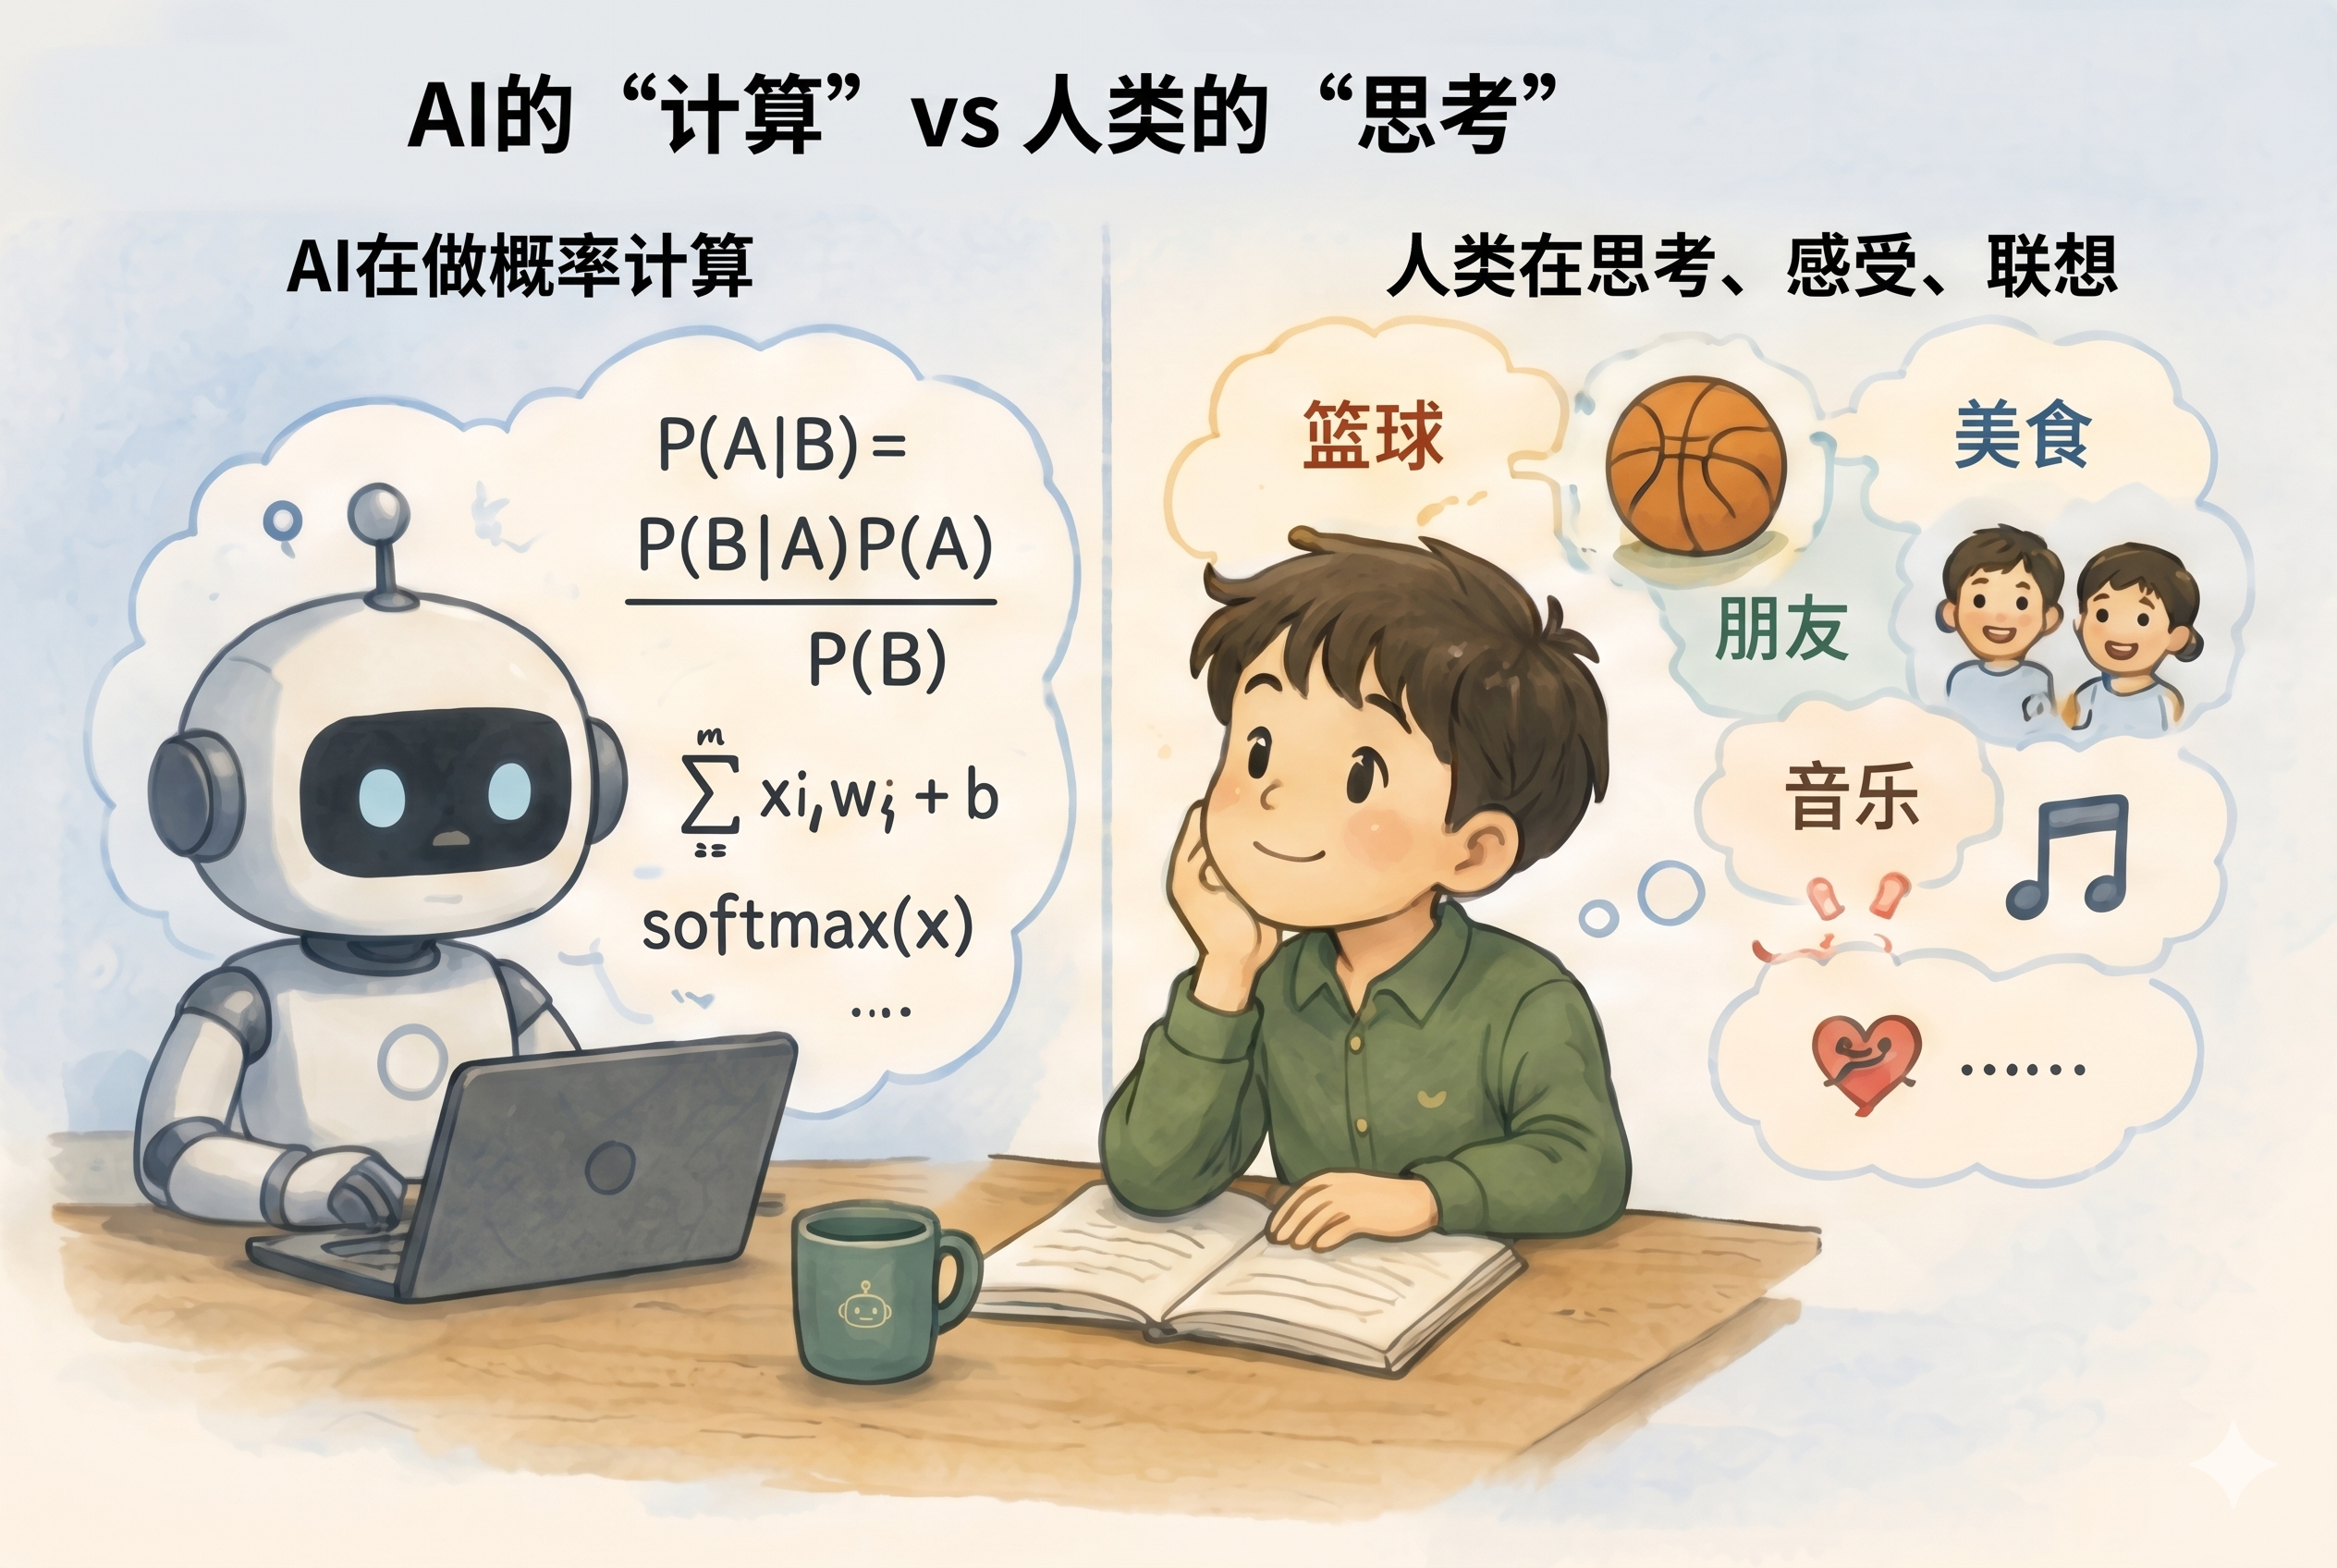
\includegraphics[width=0.88\textwidth]{images_chapter_01-03/2-5.png}
\caption*{\footnotesize\itshape\color{gray!50} 图2-5\quad 推荐系统如何从行为数据中“拼出”用户画像}
\end{figure}

理解这一点非常重要。理解了AI不会思考，你就不会对它产生不必要的恐惧——担心它哪天突然“觉醒”取代人类；你也不会对它产生不切实际的崇拜——以为它什么都知道、什么都懂。AI是工具。一个极其擅长发现规律、但完全不知道自己在做什么的工具。

接下来，我们要看看AI如何把这种“发现规律”的能力应用到视觉领域——如何从像素中“看见”世界。

\section{计算机视觉：AI学会“看见”世界}

上一节我们讲了AI如何从数据中学习规律。现在，让我们看看AI怎样把这种“学习”能力应用到视觉上——让机器“看见”世界。

2012年，一个名叫AlexNet的AI模型在ImageNet图像识别竞赛中震惊了学界。这个模型由当时还是研究生的亚历克斯·克里泽夫斯基（Alex Krizhevsky）和他的导师杰弗里·辛顿（Geoffrey Hinton）共同设计。他们用两块游戏显卡（NVIDIA GTX 580）训练了一个深度神经网络，结果在识别图片物体的比赛中，错误率从前一年的约26\%骤降至约16\%——这个巨大的飞跃令整个计算机视觉领域为之震动。从那之后，计算机视觉进入了快车道。而你可能每天都在用这项技术，却从未意识到。

\subsection{身边到处都是“长了眼睛”的机器}

大三学生小语的一天，是被机器“看”着度过的。

早晨七点半，她匆匆走过校园门禁。摄像头捕捉到她的脸，系统在不到一秒内完成了“检测人脸→提取特征→比对数据库→确认身份→开门”的全流程。她不用掏校园卡，甚至不用停下脚步。这台刷脸门禁背后的AI，已经在过去三年里“看”过她上千次——大一刚入学时她戴眼镜、留刘海；大二换了隐形眼镜、剪了短发；大三开始化淡妆——但AI始终认得她。因为它存储的不是某张特定照片，而是一组不断更新的面部特征数据。

中午在食堂，她对着支付终端眨了个眼。机器确认“活体检测通过，身份验证成功”——它能区分面前是真人还是一张照片或一段视频。

晚上她躺在床上，掏出手机。前置红外摄像头投射出三万个不可见的光点，在她脸上形成一张深度地图。面容ID在一秒内匹配成功，屏幕解锁。她点开相册，发现AI已经自动把她今天拍的37张照片按人脸分好了组——室友一个文件夹、社团朋友一个文件夹、课堂板书一个文件夹。

\begin{figure}[H]
\centering
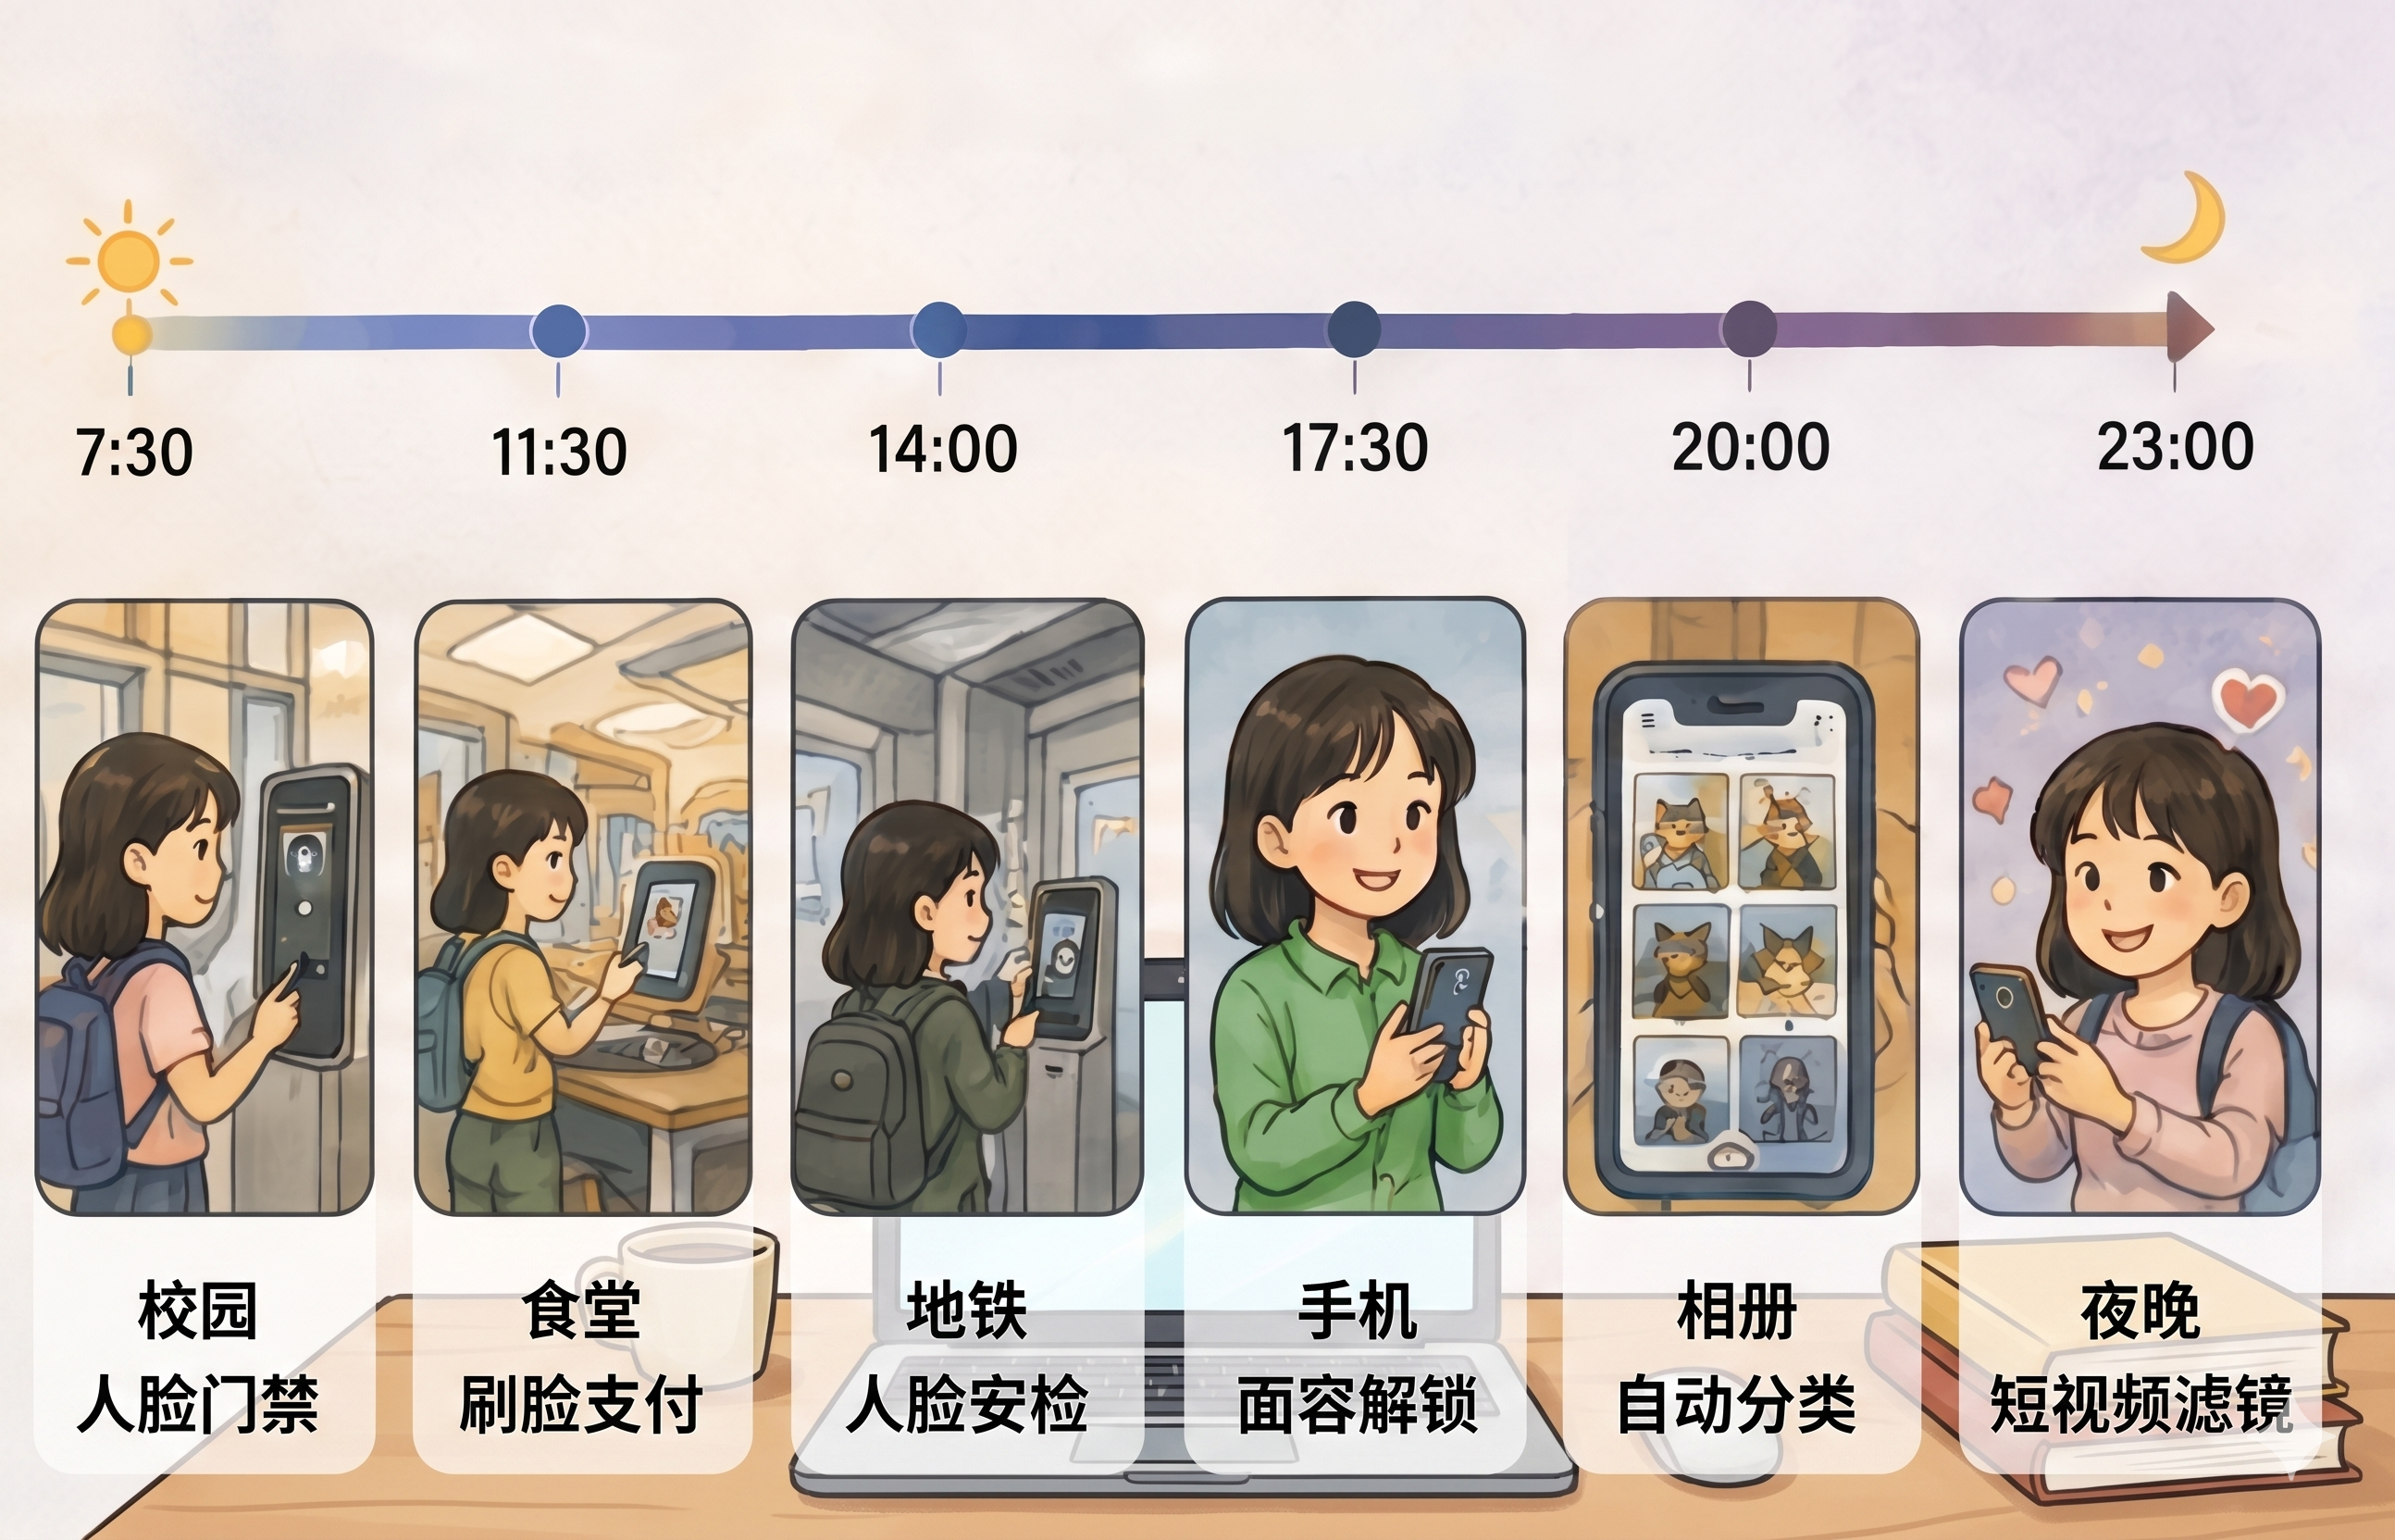
\includegraphics[width=0.88\textwidth]{images_chapter_01-03/2-6.png}
\caption*{\footnotesize\itshape\color{gray!50} 图2-6\quad 推荐系统如何从行为数据中“拼出”用户画像}
\end{figure}

这些只是小语能感知到的。在她看不见的地方，更多的“机器眼睛”正在工作：医院放射科，AI正在初筛今天的第200份CT影像，一个微小的肺结节被自动圈出并标注了坐标和风险等级；她暑假实习过的工厂流水线上，AI质检系统正以每秒几十个零件的速度扫描着产品外观，寻找纳米级别的表面瑕疵；城郊的农田上空，搭载AI摄像头的无人机正在分析作物叶片的光谱数据，判断哪一片田需要施肥、哪一片可能遭受了虫害。

那么问题来了：\textbf{一台由金属和硅片组成的机器，是怎么“看见”东西的？它看到的世界，和我们看到的一样吗？}

\subsection{人脸识别为什么有时会失败}

在回答“AI怎么看世界”之前，我们先从一个你可能也有过的困惑说起。

小语发现，白天解锁手机特别顺畅，但晚上关了灯之后，有时候怎么都解不开。戴了口罩之后，校门口的门禁偶尔认不出她。拍照时如果角度太偏，手机相册的人脸分类也会出错。

要理解这是为什么，你需要先理解一个根本性的差异：\textbf{人类“看”和AI“看”，是两件完全不同的事。}

当你看一张朋友的照片时，你的大脑自动完成了无数复杂处理——你认出了朋友的脸，感受到了他当时的情绪（开心还是尴尬），注意到了背景里的教学楼，甚至想起了那天一起吃饭的场景。你“看到”的是一个有意义的整体，你的大脑调用了你和这个人所有的交往记忆、你对人类表情的理解、你在这个世界生活了十几二十年的全部经验。

但AI面对这张照片时，它看到的只是一堆数字。一张高清照片在AI眼里是几百万个像素方格，每个像素有一个颜色数值。没有笑脸，没有回忆，没有阳光洒在桌上的温暖——只有数字。

\begin{figure}[H]
\centering
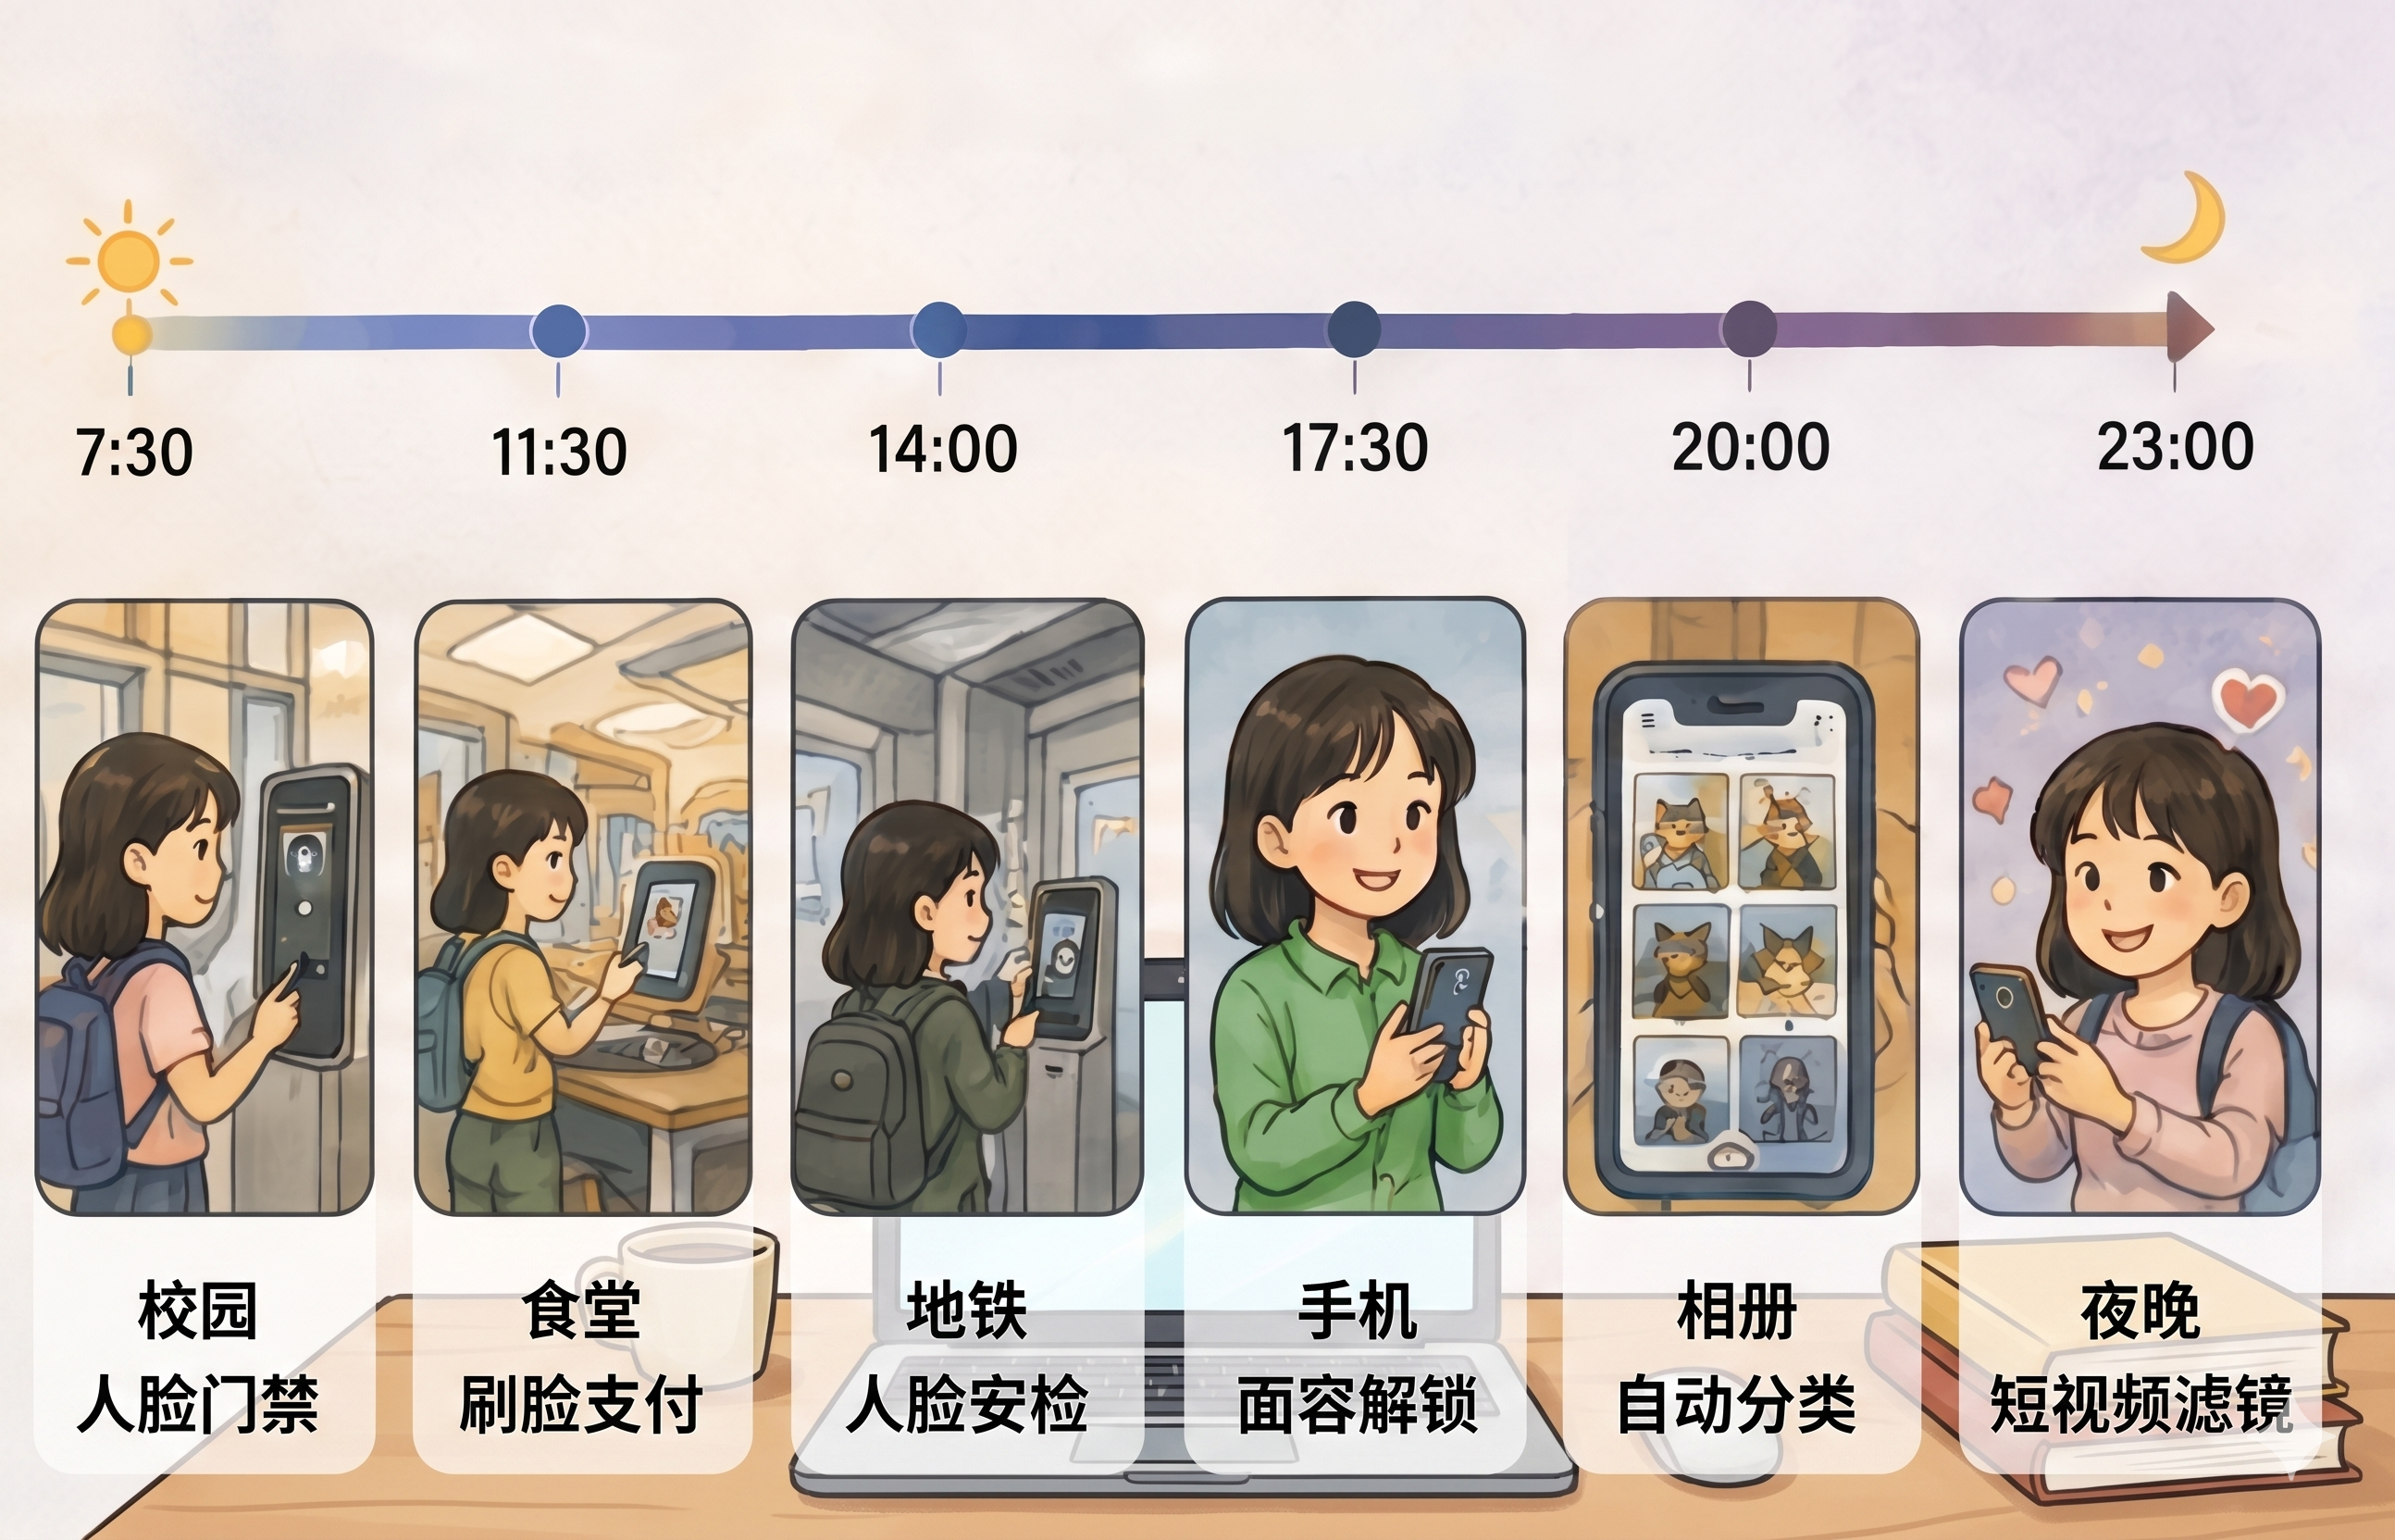
\includegraphics[width=0.88\textwidth]{images_chapter_01-03/2-6.png}
\caption*{\footnotesize\itshape\color{gray!50} 图2-2\quad 推荐系统如何从行为数据中“拼出”用户画像}
\end{figure}

AI需要从这堆数字里找规律：哪里是轮廓？哪里是边缘？颜色怎么分布？它通过分析成千上万张标注过的“人脸”图片，逐渐学会了：人脸通常有某些共同特征——两只眼睛之间大约是一个眼睛的宽度，鼻梁在脸部中间，嘴唇在鼻子下方一定距离。

现在你可以回答“为什么关灯就认不出来”了——因为黑暗中像素信息变少，AI提取到的特征不够清晰。戴口罩认不出来？因为口罩遮住了鼻子和嘴巴，AI少了一半的特征信息。角度太偏认不出来？因为AI训练时看到的大多是正面照片，侧面和仰角的样本较少，特征匹配困难。

\begin{figure}[H]
\centering
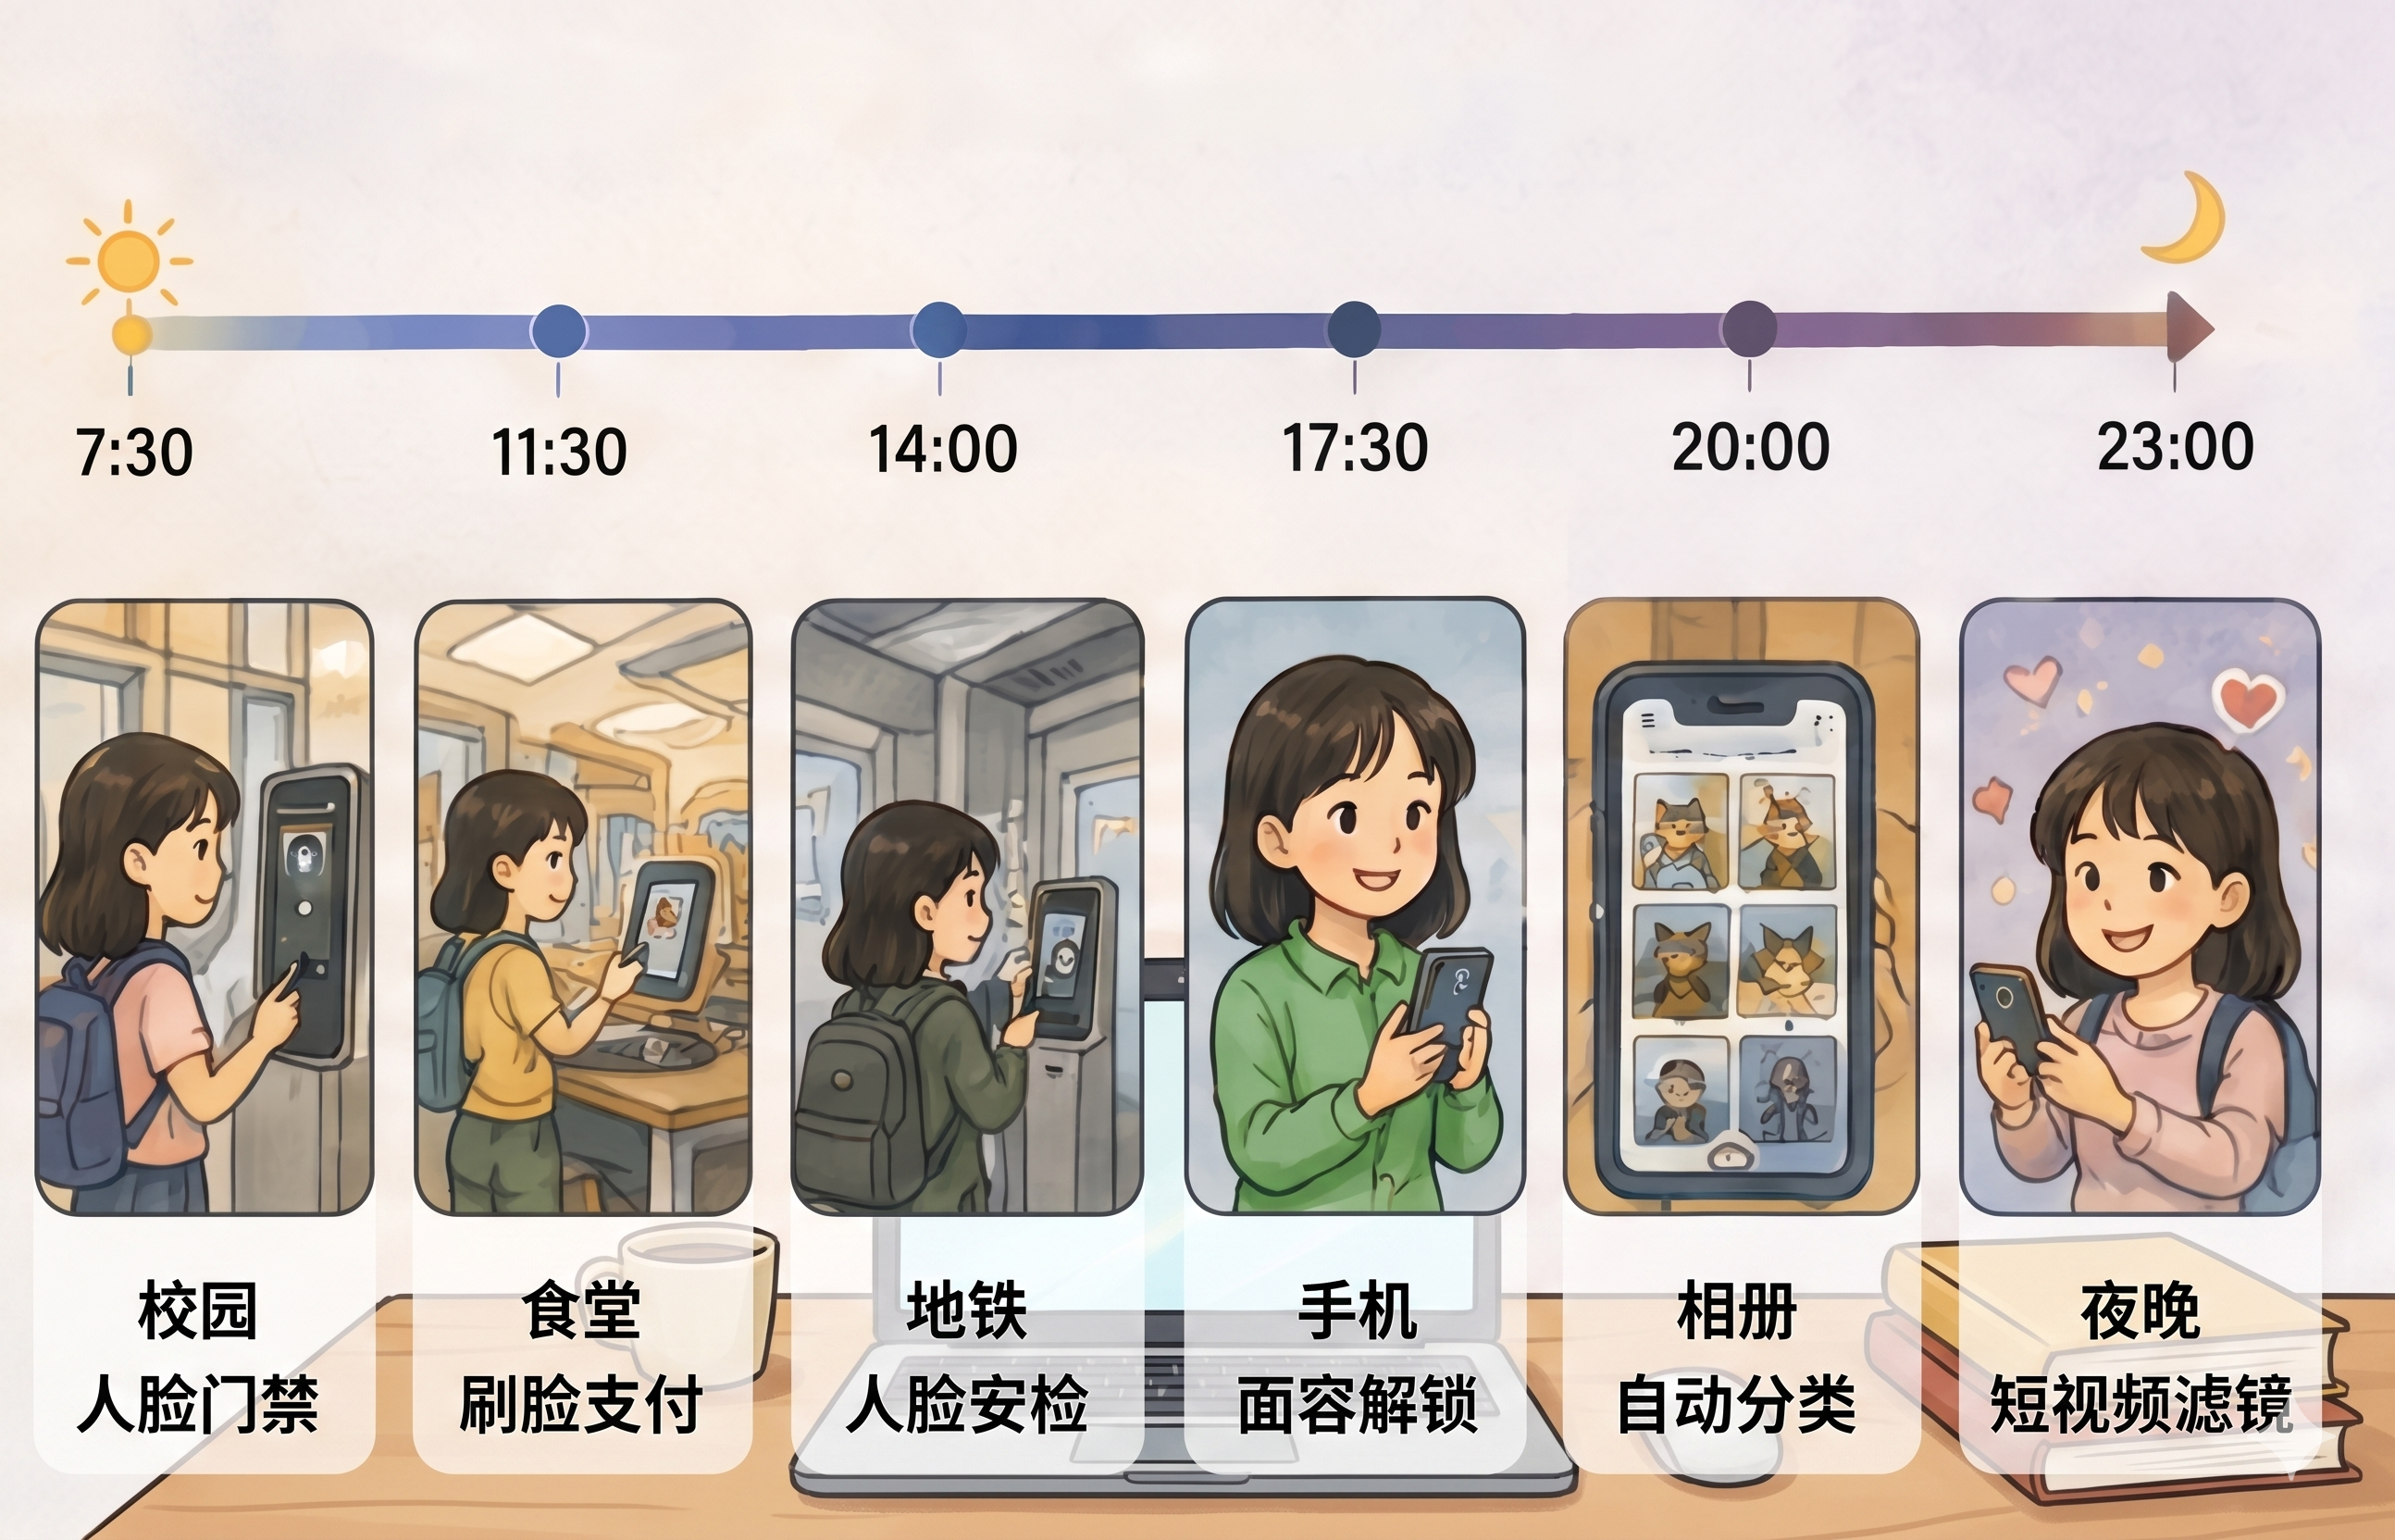
\includegraphics[width=0.88\textwidth]{images_chapter_01-03/2-6.png}
\caption*{\footnotesize\itshape\color{gray!50} 图2-2\quad 推荐系统如何从行为数据中“拼出”用户画像}
\end{figure}

所以，\textbf{AI的“看见”，本质上是一种特征匹配。} 它不是“看到”了你的脸，而是提取了你面部的一组数字特征，然后去数据库里找“有没有哪个已记录的人脸特征和这组数字高度相似”。

那么，AI具体是怎么“提取特征”的？它怎么从一堆像素数字里找出“这是眼睛”“这是鼻子”？

\subsection{计算机视觉——把图片变成AI能理解的“密码”}

让我们做一个简单实验。拿出手机，打开一张照片。用手指放大、再放大、继续放大……直到不能再放大为止。你看到了什么？

一个个纯色的小方格。这就是\textbf{像素}——数字图像的最小单位。一张1920×1080分辨率的照片，由大约200万个像素组成。每个像素有自己的颜色数值（比如R:182, G:207, B:236——这是一种淡蓝色），AI接收到的就是这200万个数字。

从这200万个数字中认出“这是我的朋友在笑”，是计算机视觉要解决的核心问题。AI做到这一点，靠的不是某种神秘的“理解”，而是一个可以被拆解为三个步骤的过程：\textbf{检测→识别→理解场景。}

\begin{figure}[H]
\centering
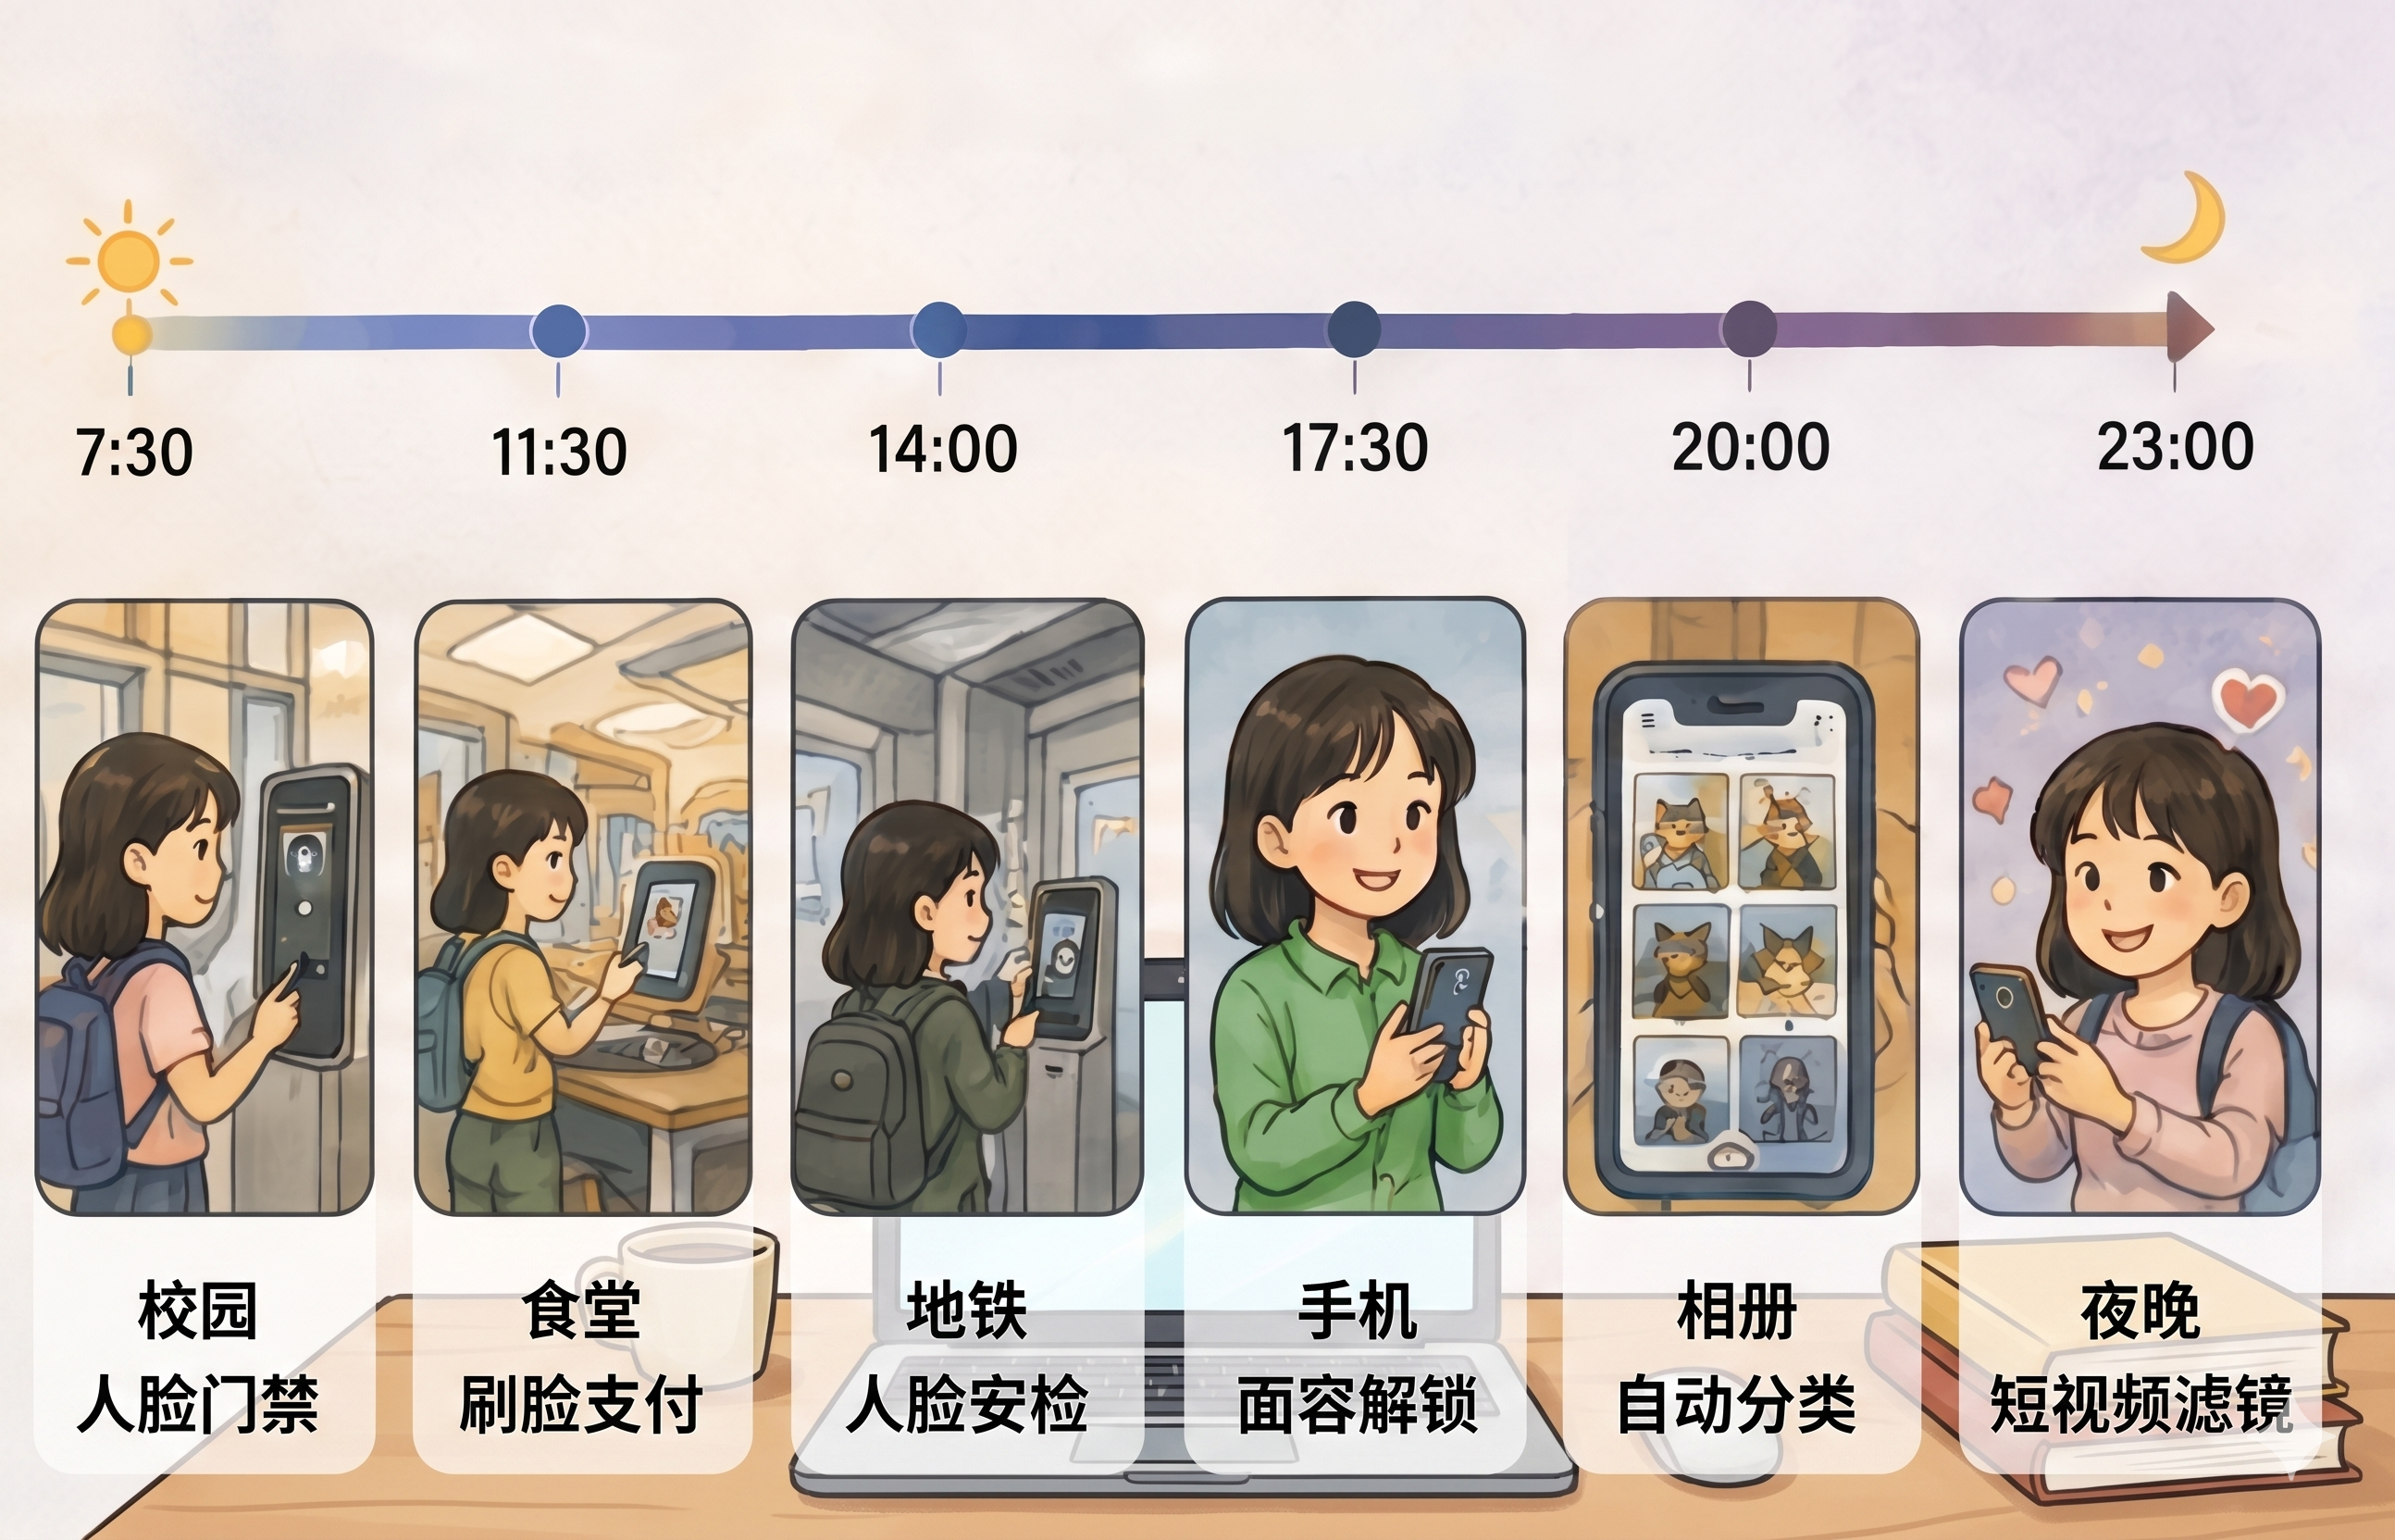
\includegraphics[width=0.88\textwidth]{images_chapter_01-03/2-6.png}
\caption*{\footnotesize\itshape\color{gray!50} 图2-2\quad 推荐系统如何从行为数据中“拼出”用户画像}
\end{figure}

\textbf{第一步：检测——画面中“有什么东西”？} AI会在图像中寻找明暗变化剧烈的区域（那里很可能是物体的边缘），寻找颜色突然过渡的线条（那里可能是物体的轮廓），寻找与周围纹理明显不同的小块（那里可能是一个独立的物体）。当这些局部特征足够多、排列成某种有规律的组合时，AI就会判断：这里可能有一个物体。

\textbf{第二步：识别——这个物体“是什么”？} AI看过数百万张标注了“这是猫”的图片后，内部参数逐渐调整，最终形成了一套对“猫的视觉特征”极其敏感的检测系统。这套系统能从各种角度、各种光照、各种品种的猫身上提取出共同的视觉模式——某种耳朵轮廓的曲率范围、某种眼睛间距与脸宽的比例、某种毛发纹理的统计特征。AI自己也不知道这些模式“意味着”什么，它只知道当这些特征同时出现时，输出“猫”这个标签的概率最高。

\textbf{第三步：场景理解——这些物体之间“是什么关系”？} 这是最难的一步。AI能认出画面中有一个女孩、一个气球、一片草地，但“女孩在公园里高兴地拿着气球”——这个融合了物体关系、场景属性、情绪判断的综合理解，AI目前仍然非常吃力。

\begin{knowledgebox}
\textbf{特征提取——侦探在犯罪现场寻找线索}

AI从像素中提取有用信息的过程，在术语上叫\textbf{特征提取}。你可以把它想象成一位侦探调查犯罪现场：他不需要把整个房间原封不动地搬回警察局，只需要带走关键的指纹、血迹样本、几帧监控录像。AI看图也是同样的逻辑——它不看整张照片，而是提取那些最关键的特征（边缘、形状、颜色分布），然后与数据库中已知物体的“特征档案”做比对。这种“只见树木、不见森林”的做法，正是AI视觉效率极高的原因，也是它时常闹笑话的根源。
\end{knowledgebox}

理解了这三步，你就能回答本节开头的问题了：\textbf{AI不是真正“看见”了世界，它只是在提取视觉特征并进行模式匹配。} 它看到的是数字、是统计规律，而不是物体本身。它不知道“猫”摸起来是什么感觉，“阳光”照在脸上有多温暖，“微笑”背后是什么心情。它只知道当像素排列成某种模式时，输出“猫”的标签；排列成另一种模式时，输出“微笑”的标签。

接下来你可能想知道：既然AI这么擅长模式匹配，它在现实生活中到底能派上什么用场？

\subsection{计算机视觉应用案例}

计算机视觉是当前应用最广泛的AI技术之一。在医疗领域，它帮助医生从CT和X光片中筛查早期病灶；在工业领域，它在生产线上以微米级精度检测产品瑕疵；在农业领域，它通过无人机航拍分析作物长势和病虫害；在体育领域，它追踪运动员的每一个关节动作优化训练方案；在交通领域，它让自动驾驶汽车“看”清路况；在安防领域，它实时分析监控视频识别异常行为；在你的手机里，它自动分类相册照片、解锁屏幕、为短视频添加特效滤镜。

下面，我们通过三个来自不同领域的案例，看看计算机视觉具体是如何运作的。

\subsubsection*{案例1：AI怎样帮助医生发现早期癌症}

2023年秋天，江苏。一位50岁的男性因轻微咳嗽去医院就诊。常规X光胸片显示肺部纹理略增粗，放射科医生判断“无明显异常”，建议按支气管炎处理。

然而，这家医院同时部署了AI辅助影像筛查系统。在医生离开阅片室之后，AI自动重读了同一张X光片。它在右肺上叶区域标注了一个直径约7毫米的微小结节。这个结节的密度只比周围肺组织高出不到10\%，在肉眼直视下几乎无法分辨——就像在灰布上找一块略浅一点的灰斑。AI将其标注为“高风险：建议CT进一步检查”。

正是这个冷冰冰的标注提醒了医生。患者接受了CT扫描，结果确认那是一个早期肺腺癌病灶——直径不到8毫米，尚未扩散，完全可以手术切除。三个月后，手术成功，患者康复。

这个案例里的AI，训练数据来自全国多家三甲医院超过一百万例已标注的肺部CT和X光影像。在训练过程中，它学会了识别那些连资深放射科医生也可能漏掉的细微视觉模式：某些特定的纹理组合、某些特定形态的密度变化、某些特定位置的微小不对称。

但AI也不是完美无缺的。在另一组测试中，同一套系统在22\%的病例中将良性钙化点误判为可疑结节，在约5\%的病例中将早期癌变漏判为正常。这就是为什么它只做“初筛”，最终诊断必须由医生来做。AI不会替代医生，但它让医生多了一双永不疲倦、不会因为阅片到第200张而注意力涣散的“第二双眼睛”。

\subsubsection*{案例2：AI质检员怎样守护你的手机屏幕}

你每天滑动的手机屏幕，在出厂前要经过AI质检的严格把关。

在手机玻璃盖板生产线上，每块盖板只有零点几毫米厚，却要经过数十道工序。任何一道工序中出现划痕、气泡、色差或边缘崩缺，都会影响最终产品的质量。过去，这条质检线靠人眼来完成——质检员坐在强光灯下，一块一块地翻看玻璃盖板，寻找微米级别的瑕疵。一个人一天要看上千块，眼睛疲劳后很容易漏检。而且人跟人之间的判断标准也不完全一致——有人严格，有人宽松。

现在，高速工业相机以微米级精度扫描每一块盖板，AI系统实时分析图像，检测划痕、气泡、色差和边缘缺陷。它不会疲劳，不会因为今天心情不好而误判，检测标准也不会因人而异。在富士康的某些产线上，AI质检系统每天检测超过百万个零件，漏检率远低于传统人工质检。

更有意思的是，AI质检还能做“预防性分析”。如果系统发现某一批次的产品中某个特定位置反复出现同类型瑕疵，它会自动发出预警——这可能意味着生产线上某个环节出了微小的问题，比如注塑模具的某个角落开始磨损。在问题变得严重之前就被发现和修正，避免了大量次品的产生。

\subsubsection*{案例3：AI怎样帮农民“看”庄稼}

在黑龙江的一家大型农场里，搭载多光谱摄像头的无人机正飞过一望无际的麦田。

无人机拍下的不是普通照片，而是多光谱图像——它能捕捉到人眼看不到的近红外光反射。健康的作物叶片会强烈反射近红外光，而缺水、缺肥或遭受病虫害的作物，其光谱反射特征会发生变化。这种变化在肉眼能察觉之前就已经在光谱数据中显现了。

AI系统分析这些光谱数据，判断每一块田地的作物健康状况。哪里缺水、哪里缺氮肥、哪里可能出现了早期病虫害——AI生成一张“农田处方图”，用不同颜色标注不同区域的需求。施肥机按照这张图的指引，在需要的地方精准施入所需量的肥料，而不是整片地均匀撒播。

这套系统让施肥量减少了约15\%，同时产量提升了约8\%。因为在过去，农民只能凭经验整片地施同样多的肥——有些地方施多了浪费，有些地方施少了减产。AI让农业从“看天吃饭”变成了“看数据吃饭”，每一株作物都得到了最适合它的照料。

\begin{knowledgebox}
\textbf{多光谱图像——植物健康的“透视镜”}

普通相机只能记录红、绿、蓝三种颜色，而\textbf{多光谱相机}能看到人眼看不见的近红外光。健康植物在近红外波段会强烈反射——就像给自己拍了一张“健康证明”。一旦植物缺水或患病，反射率就会下降。AI通过分析这些肉眼不可见的光谱变化，可以在症状显现之前就发现问题。这项技术最早用于卫星遥感监测大范围植被，如今随着无人机成本下降，已经飞入了寻常农田。
\end{knowledgebox}

\subsection{AI真的“看懂”图片了吗}

先看一个经典翻车现场。

一位研究者做了一个实验：他找了一张哈士奇站在雪地里的照片，让AI判断照片里是什么动物。AI信心十足地给出答案：“狼。”为什么？因为AI训练数据中狼的照片大多背景是雪地或森林。它没有学会“狼的生物学特征”，它学会的是“雪地背景+黑白毛色≈狼”。

类似的故事还有：一只猫穿上了狗的万圣节服装（衣服上有狗耳朵造型），AI判断为“狗”——因为它提取的关键特征是“狗耳朵形状的轮廓”。一张毕业照，人类看到的是青春、友谊和离别，AI看到的是“一群人穿着相似的衣服站成几排”。

\begin{figure}[H]
\centering
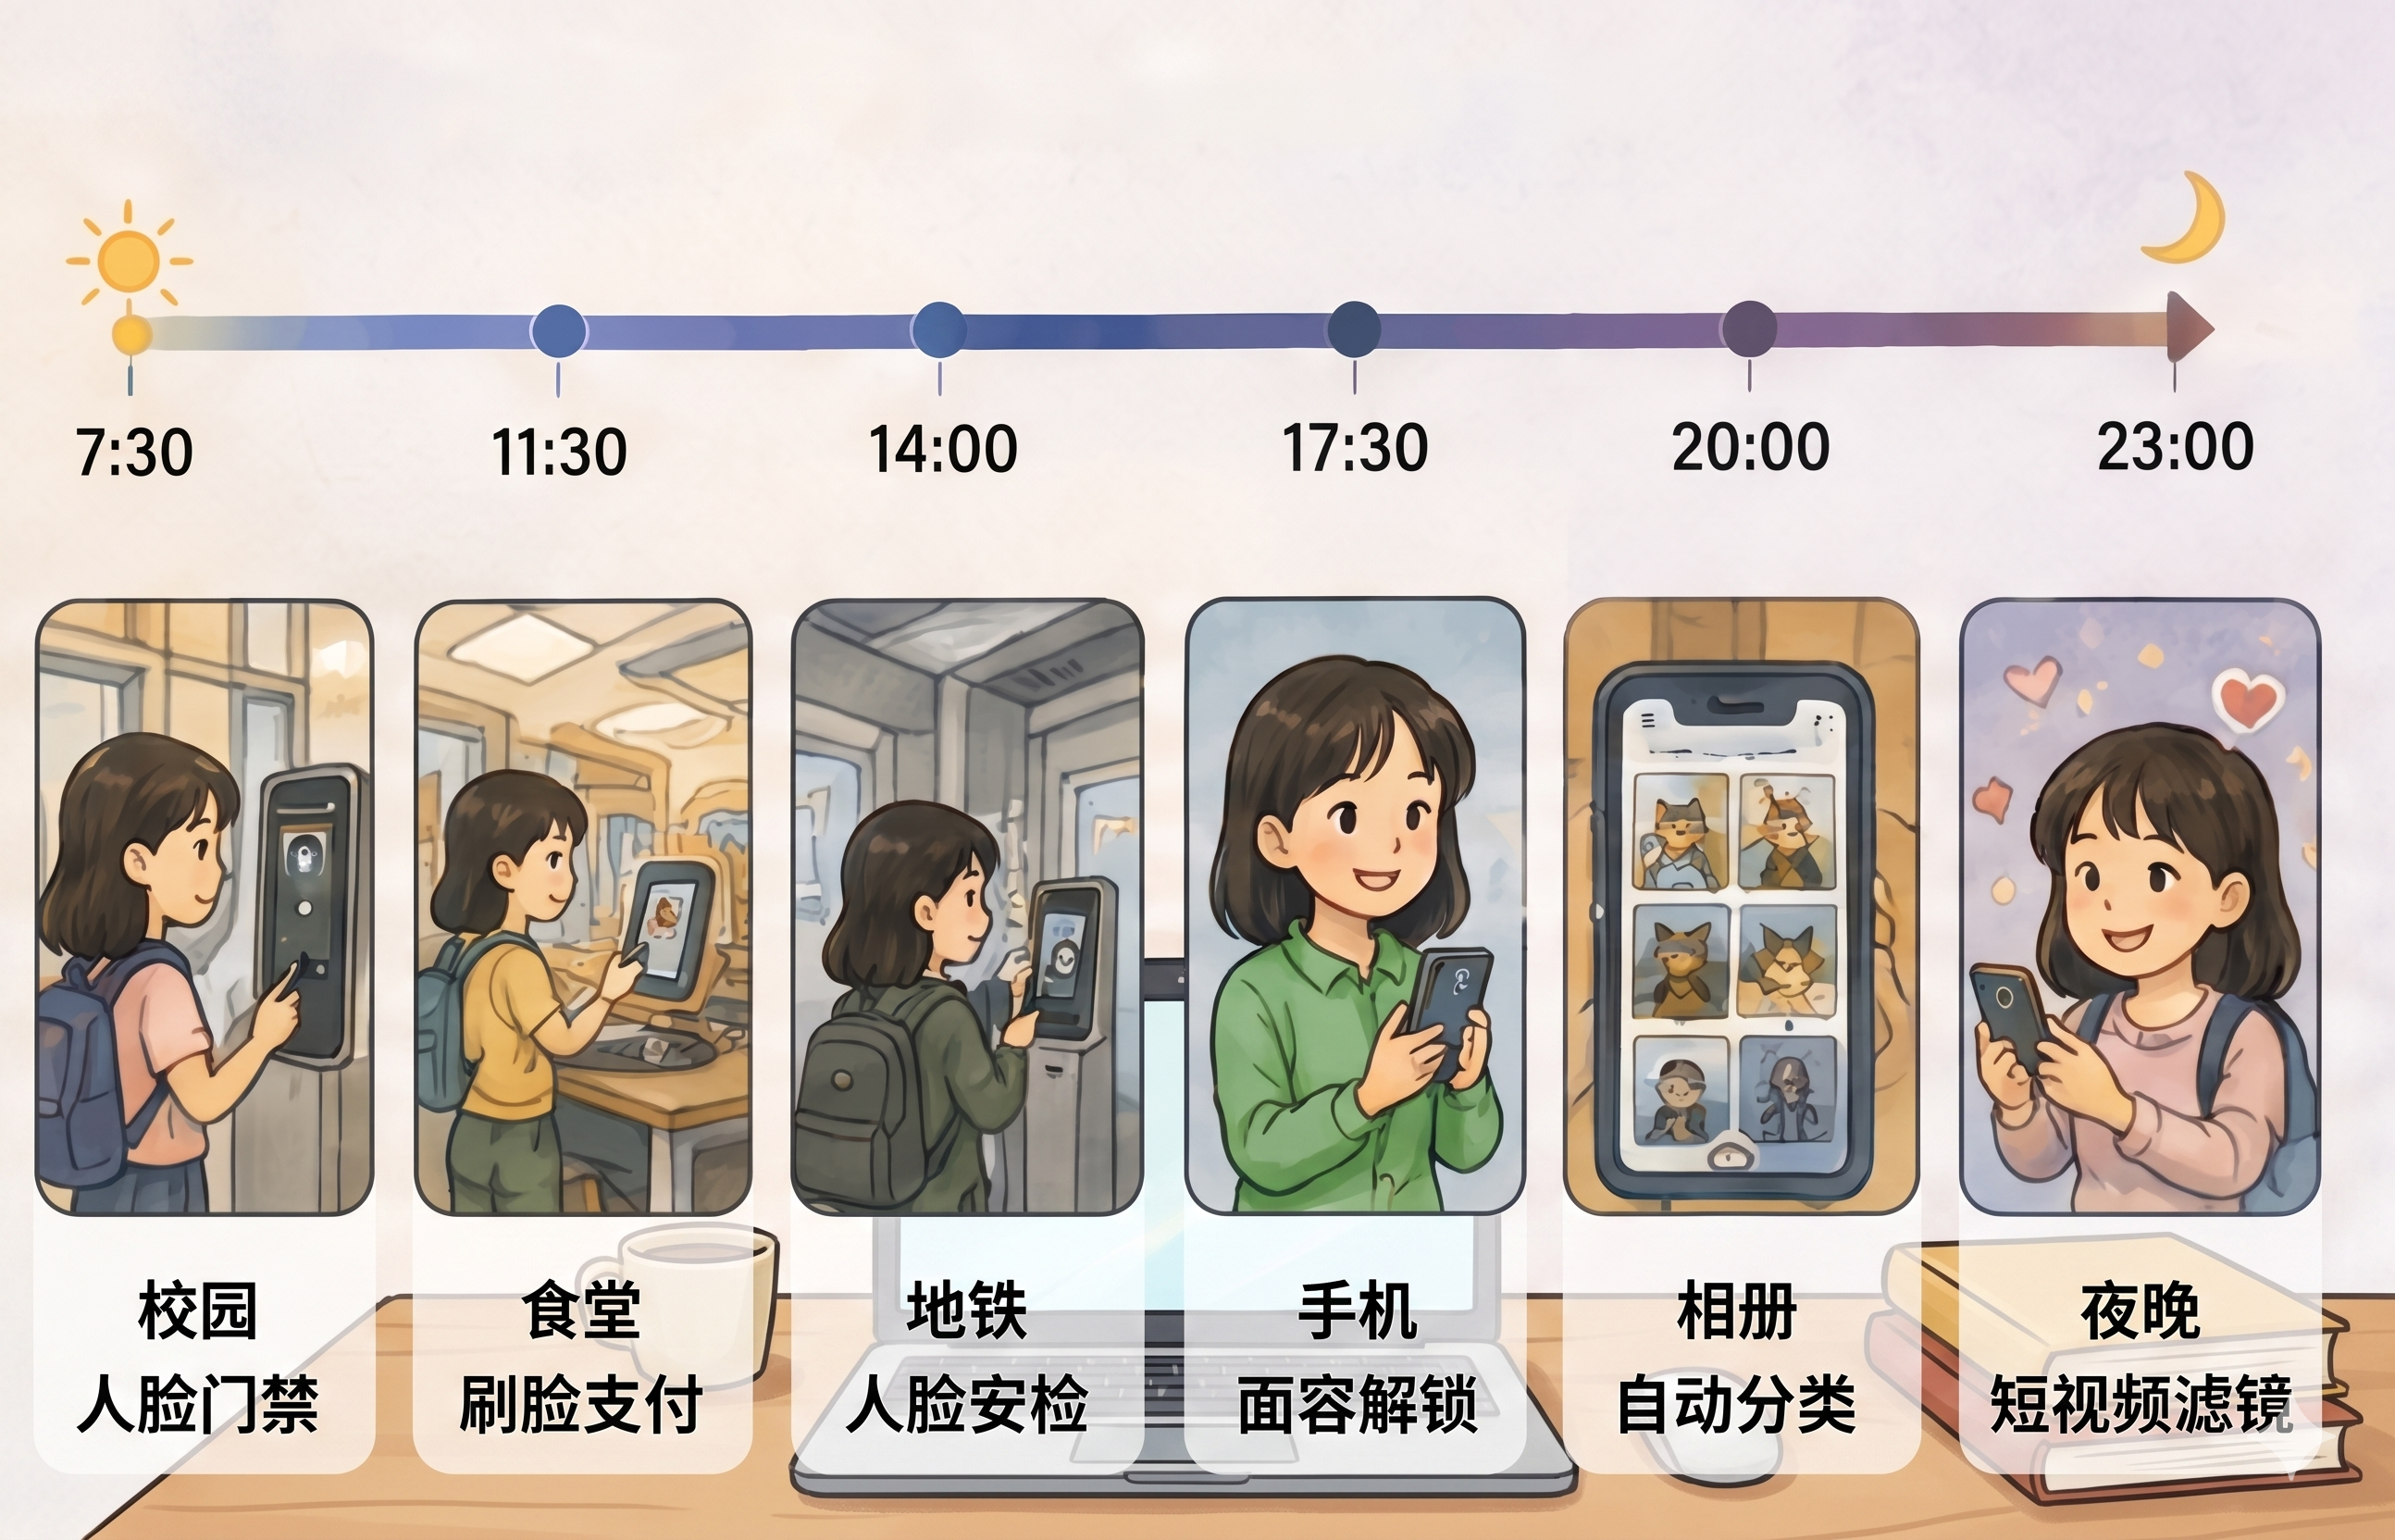
\includegraphics[width=0.88\textwidth]{images_chapter_01-03/2-6.png}
\caption*{\footnotesize\itshape\color{gray!50} 图2-2\quad 推荐系统如何从行为数据中“拼出”用户画像}
\end{figure}

这些翻车案例揭示的，是计算机视觉的三条根本局限：

第一，\textbf{识别不等于理解。} AI能告诉你“这是一张毕业照”，但它不知道毕业意味着什么——它不知道这群人在一起生活了四年，不知道有人在快门按下时忍着眼泪，不知道十年后这张照片会被反复翻出来看。AI看到的只是像素和特征，不是意义和情感。

第二，\textbf{严重依赖训练数据。} AI只“认识”它“见过”的东西。如果训练数据里黑猫的照片太少，AI面对黑猫就可能犹豫或出错。

\begin{funbox}
\textbf{当人脸识别遇上肤色差异——一个MIT实验室的发现}

2018年，麻省理工学院（MIT）媒体实验室的研究生乔伊·布兰维尼（Joy Buolamwini）在做人脸识别实验时，发现了一个让她震惊的问题。当时市面上的主流人脸识别系统在她脸上完全不起作用——她是黑人女性。她尝试了各种方法：调整灯光、改变角度、摘下眼镜——系统始终无法稳定识别她的脸。

百思不得其解的她做了一个实验：在脸上戴上一个白色面具。结果系统立刻成功识别了——识别的是面具，而不是她的脸。

这个发现后来催生了著名的“Gender Shades”研究。研究结果显示，在当时的主流商业人脸识别系统中，浅肤色男性的识别错误率最低（不到1\%），而深肤色女性的错误率最高（可达35\%）。原因不是算法“歧视”——而是训练数据严重失衡。这些系统在训练时使用了大量浅肤色人脸样本和大量男性人脸样本，深肤色女性样本严重不足。AI只是忠实地反映了它“见过”的世界。

布兰维尼的故事后来被广泛报道，并直接推动了多家科技公司改进人脸识别系统的训练数据多样性。它告诉我们：AI的“眼睛”看到的世界，取决于人类给它看了什么样的世界。
\end{funbox}

2018年，MIT的研究者发现，市面上的主流人脸识别系统在识别浅肤色男性时错误率不到1\%，但在识别深肤色女性时错误率可高达35\%——原因不是算法“歧视”，而是训练数据中深肤色女性样本太少。

第三，\textbf{没有常识和推理能力。} AI看到一张“人在水里骑自行车”的图片不会觉得奇怪——因为它不知道水面不能骑车。它没有在现实世界中生活过一天，不知道水是液体、液体会流动、人站在液体上会沉下去。这些对人类来说最基本不过的常识，AI统统没有。

所以，回到本节标题的问题：\textbf{AI真的“看懂”图片了吗？} 答案是没有。它没有“看懂”，它只是在一个极其庞大的视觉特征数据库里，完成了极其高效的模式匹配。“识别不等于理解”——这七个字，是你理解计算机视觉边界的核心钥匙。

接下来，我们要进入一个更让人惊叹的领域——\textbf{自然语言处理}。如果计算机视觉是AI的“眼睛”，那自然语言处理就是AI的“嘴巴和耳朵”。我们将看到AI是如何学会“说话”的，以及——它真的“理解”自己说的话吗？

\section{自然语言处理：AI如何理解和生成语言}

2018年，大三学生小杨去英国交换。出发前，他自信满满地在手机里下载了一款翻译App。落地伦敦后第一次去超市，他想买洗发水，但分不清货架上哪瓶是洗发水、哪瓶是护发素——全是英文。他掏出手机，对着瓶身上的说明拍了张照。翻译结果：“头发营养供应者。使用后，您的头发将拥有丰富的早餐体验。”

丰富的早餐体验？小杨愣了五秒。“我只是想知道这是洗发水还是护发素啊！”

那个年代，社交媒体上流行一个词来形容AI的语言能力：\textbf{人工智障}。早期机器翻译经常闹笑话，智能客服只会回复预设话术，语音助手连“播放周杰伦的歌”都经常听成“播放周结论的歌”。

然后，事情突然变了。2022年11月30日，ChatGPT发布。两个月内，用户突破一亿——成为人类历史上增长速度最快的消费级应用。社交媒体上迅速涌入大量惊叹：有人让它写论文提纲，有人让它讲解高数题，有人凌晨三点和它聊失恋，得到了比一些真人朋友还温柔的回应。

AI突然变得“能说会道”了。它是怎么做到的？

\subsection{AI突然变得“能说会道”了}

让我们从“过去”说起。

早期机器翻译的典型翻车现场可以写成一本书。一句中文“好好学习，天天向上”曾被翻译成“good good study, day day up”——每个单词都对，但拼起来完全不像人话。早期智能客服更是令人崩溃。你问“这门课还有名额吗”，对面永远回复“您好，请先选择您要查询的学期”。早期语音助手也只能完成“打开音乐”“设闹钟”这类简单指令——稍微复杂一点就“我不太明白你在说什么”。

这就是几年前人机语言交互的普遍水平。AI能完成一些简单的语言任务——关键词搜索、固定模板回复、基础翻译——但只要超出预设范围，立刻“智力归零”。

\textbf{然后，2022年底，一切都变了。}

\begin{figure}[H]
\centering
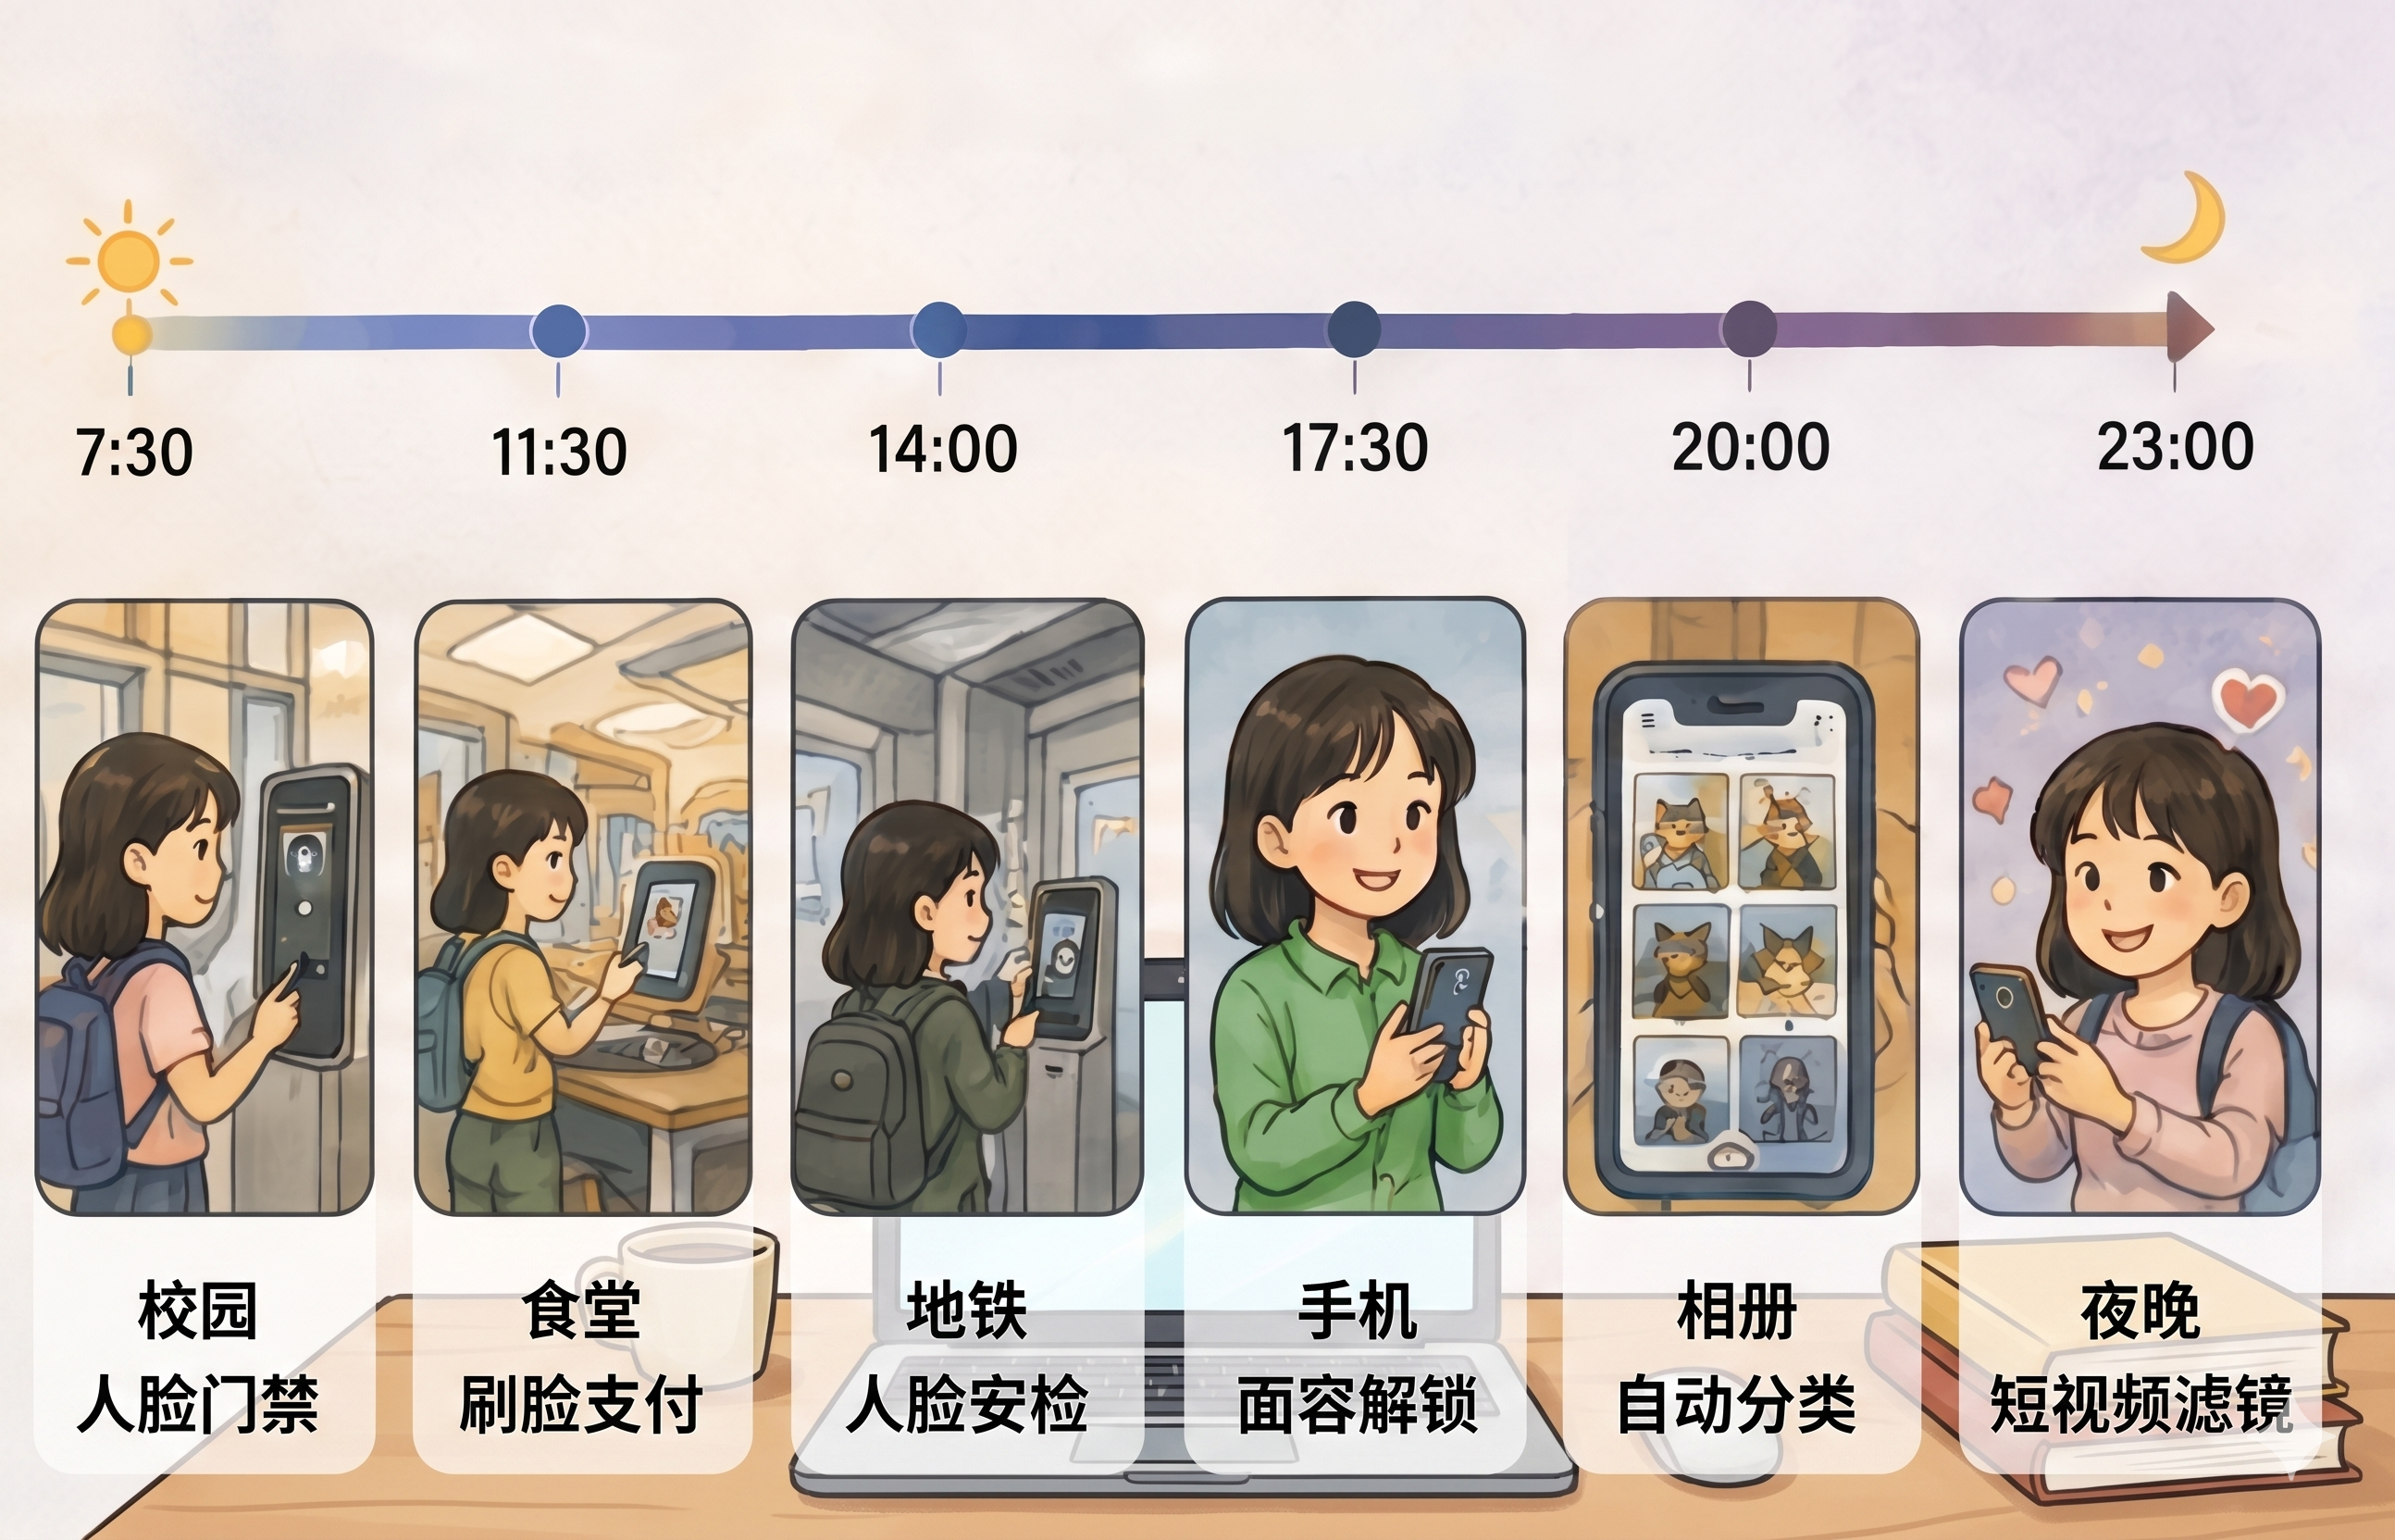
\includegraphics[width=0.88\textwidth]{images_chapter_01-03/2-6.png}
\caption*{\footnotesize\itshape\color{gray!50} 图2-2\quad 推荐系统如何从行为数据中“拼出”用户画像}
\end{figure}

ChatGPT发布后两个月用户破亿。它的出现让大多数人第一次亲身体验到AI“像人一样对话”是什么感觉。紧随其后，DeepSeek、豆包、Kimi等国产大模型迅速进入校园和办公场景。学生用AI整理课堂笔记、总结论文核心观点、生成演讲稿、润色简历。职场人用AI自动生成会议纪要、整理周报。

一位大四学生分享了他的体验：“我上传了一篇十几页的英文论文，跟AI说‘帮我总结核心观点，顺便整理一下考试可能考的重点’。几十秒后，它不仅总结好了，还生成了一个思维导图。以前可能要花两三个小时的事，现在几分钟搞定。”

过去，AI大多只能完成“单一任务”——翻译软件只管翻译，搜索引擎只管搜索，客服机器人只能回复预设话术。而今天的大模型，同一个AI既能聊天、翻译、总结文章，又能写代码、生成PPT、辅导学习。它开始具备\textbf{连续对话、理解上下文、模仿语气和跨任务协作}的能力。

那么问题来了：\textbf{语言明明如此复杂，AI为什么突然能和人顺畅交流了？它真的“听懂”我们了吗？}

\subsection{语言如此复杂，AI为何能“对答如流”}

在回答这个问题之前，让我们先承认一件事：\textbf{理解语言，是人类最了不起的能力之一，也是AI最难以攻克的难题之一。}

想想看，你每天都在接触多复杂的语言现象：同一句话在不同场景下含义完全不同——“你可真行”，有时是佩服，有时是讽刺。网络热词更新比你追的剧还快——从“绝绝子”到“yyds”到“显眼包”。很多人说话根本不按语法来——“你看那个，就是那个，懂我意思吧？”人类瞬间能懂，但机器如果逐字分析，只能一脸茫然。

但AI用一种“绕开理解”的方式，解决了这个难题。它不是像人类那样先理解再表达，而是用统计方法直接“猜”——猜在给定上下文中，下一个词最可能是什么。

\textbf{AI是怎么做到的？答案是：沉浸式学习。}

还记得2.1节我们怎么讲“机器学习”的吗？AI不是靠人工编写规则，而是通过大量例子自己找规律。自然语言处理也是一样。一个孩子学会说中文，不是靠背诵语法书，而是在语言环境中日复一日地听、模仿、被纠正。AI学习语言也是类似过程：它会“阅读”海量互联网文本——新闻、小说、论文、网页、百科、聊天记录、代码、影评……在阅读过程中，它逐渐学会了哪些词语经常一起出现，哪些表达对应哪些语气，什么样的句子结构更符合人类说话习惯。

一个直观类比：想象一个留学生在中国住了二十年。他没上过一节正经中文课，不学语法，不背单词。但他的室友是中国人，他天天一起吃饭聊天；他看中国新闻，刷中国社交媒体，逛中国菜市场。二十年后，他能用中文开玩笑，能听懂“阴阳怪气”，甚至会说方言。AI的语言学习，就是这种“沉浸式学习”的超级加强版——它不是在现实中生活了二十年，而是在几十亿页的文本中“生活”了几个月。

所以，\textbf{AI所谓“听懂语言”，本质并不是拥有真正的人类理解能力，而是通过在海量语言数据中学习规律，对“下一句最可能说什么”做极其精准的概率预测。} 它像一个语言界的“超级模仿者”——模仿得太像了，以至于我们产生了“它真的懂了”的错觉。

那么，AI具体是怎么学习语言规律的？为什么大模型让AI的语言能力突然变得这么强？

\begin{funbox}
\textbf{“心不在焉，不见泰山”——一个经典翻译翻车故事}

在机器翻译的发展史上，有一个广为流传的经典翻车案例。研究者想测试早期的机器翻译系统，输入了一句英文谚语：

“Out of sight, out of mind.”

这句话的本意是“眼不见，心不烦”——见不到的东西就不会惦记。早期的机器翻译系统逐词翻译后给出了英文到俄文的翻译，然后再从俄文翻译回英文。结果变成了：

“Invisible and insane.”

“隐形且疯狂。”

这个结果离原意十万八千里。研究者们捧腹大笑，但这个案例背后揭示的是一个深刻的难题：语言不是单词的简单拼合。同一个短语在不同语境下可能有完全不同的含义，而早期AI完全不具备“理解语境”的能力。今天的AI在这个问题上已经有了巨大的进步——但它是怎么做到的？答案就在下一节要讲的大语言模型中。
\end{funbox}

\subsection{大语言模型——AI的“超级语言大脑”}

要理解大模型，先理解它“大”在哪里。

\textbf{什么是自然语言处理（NLP）？} 简单说，就是“让计算机处理和理解人类语言”的技术。它涵盖了所有和语言相关的AI能力：文字识别、语音转文字、机器翻译、语义分析、对话系统、文本生成。

在ChatGPT出现之前，NLP系统通常只能完成某一个固定任务。翻译软件只会翻译，不会聊天；搜索引擎只会搜网页，不会总结。这个阶段的AI，像只会做一道菜的厨师——你点他拿手的青椒肉丝，他做得又快又好；但你要番茄炒蛋，他只能说“抱歉，我的菜单上没有这道菜”。

\textbf{大模型的出现改变了这一切。}

“大语言模型”（Large Language Model, LLM）中的“大”是关键。过去的AI模型，参数量可能只有几百万到几千万。而ChatGPT背后的GPT-3模型，参数达到了1750亿。后来的GPT-4据说有数万亿参数。参数越多，模型就能学习越复杂的语言规律——就像一个只读过课本的学生，和读过整个图书馆的学生，对世界的理解深度当然不同。

\begin{knowledgebox}
\textbf{参数——AI的“记忆单元”}

\textbf{参数}可以理解为AI模型内部的“记忆单元”或“知识存储位”。每个参数存储着模型从训练数据中学到的一点点信息。当参数只有几百个时，AI只能记住最简单的模式（比如“红色圆形”和“蓝色方形”的区别）。当参数达到1750亿时，AI就能记住极其复杂的语言模式——比如“在悲伤的语境下，应该用什么样的语气和措辞”。GPT-3的1750亿个参数，如果每个参数写在一张便签纸上，这些便签纸摞起来比珠穆朗玛峰还高。换句话说，你每天跟AI聊天，其实是在跟一座“便签纸山”对话。
\end{knowledgebox}

大语言模型学习了几乎所有公开网页文本、大量书籍和文学作品、程序代码、多语言内容。结果是什么呢？同一个AI，既能帮大学生总结论文、帮程序员写代码、帮文案写广告语、帮厨师推荐菜谱搭配、帮老师出考试题。这种从“单一技能”到“通用能力”的跨越，就是大模型带来的核心变化。

\textbf{那么大模型到底是怎么工作的？} 用一句话概括：它本质上是在做“预测下一个最可能出现的词”。当你输入“今天天气很好，我想去\_\_”，它根据学过的语言规律，推断后面最可能接什么词——“公园”“散步”“旅行”“打球”……它选择一个最合理的输出。然后它再根据“今天天气很好，我想去公园”，预测再下一个词。这个过程听起来简单，但当模型足够大、训练数据足够多时，它就展现出了令人惊叹的语言能力。

\begin{figure}[H]
\centering
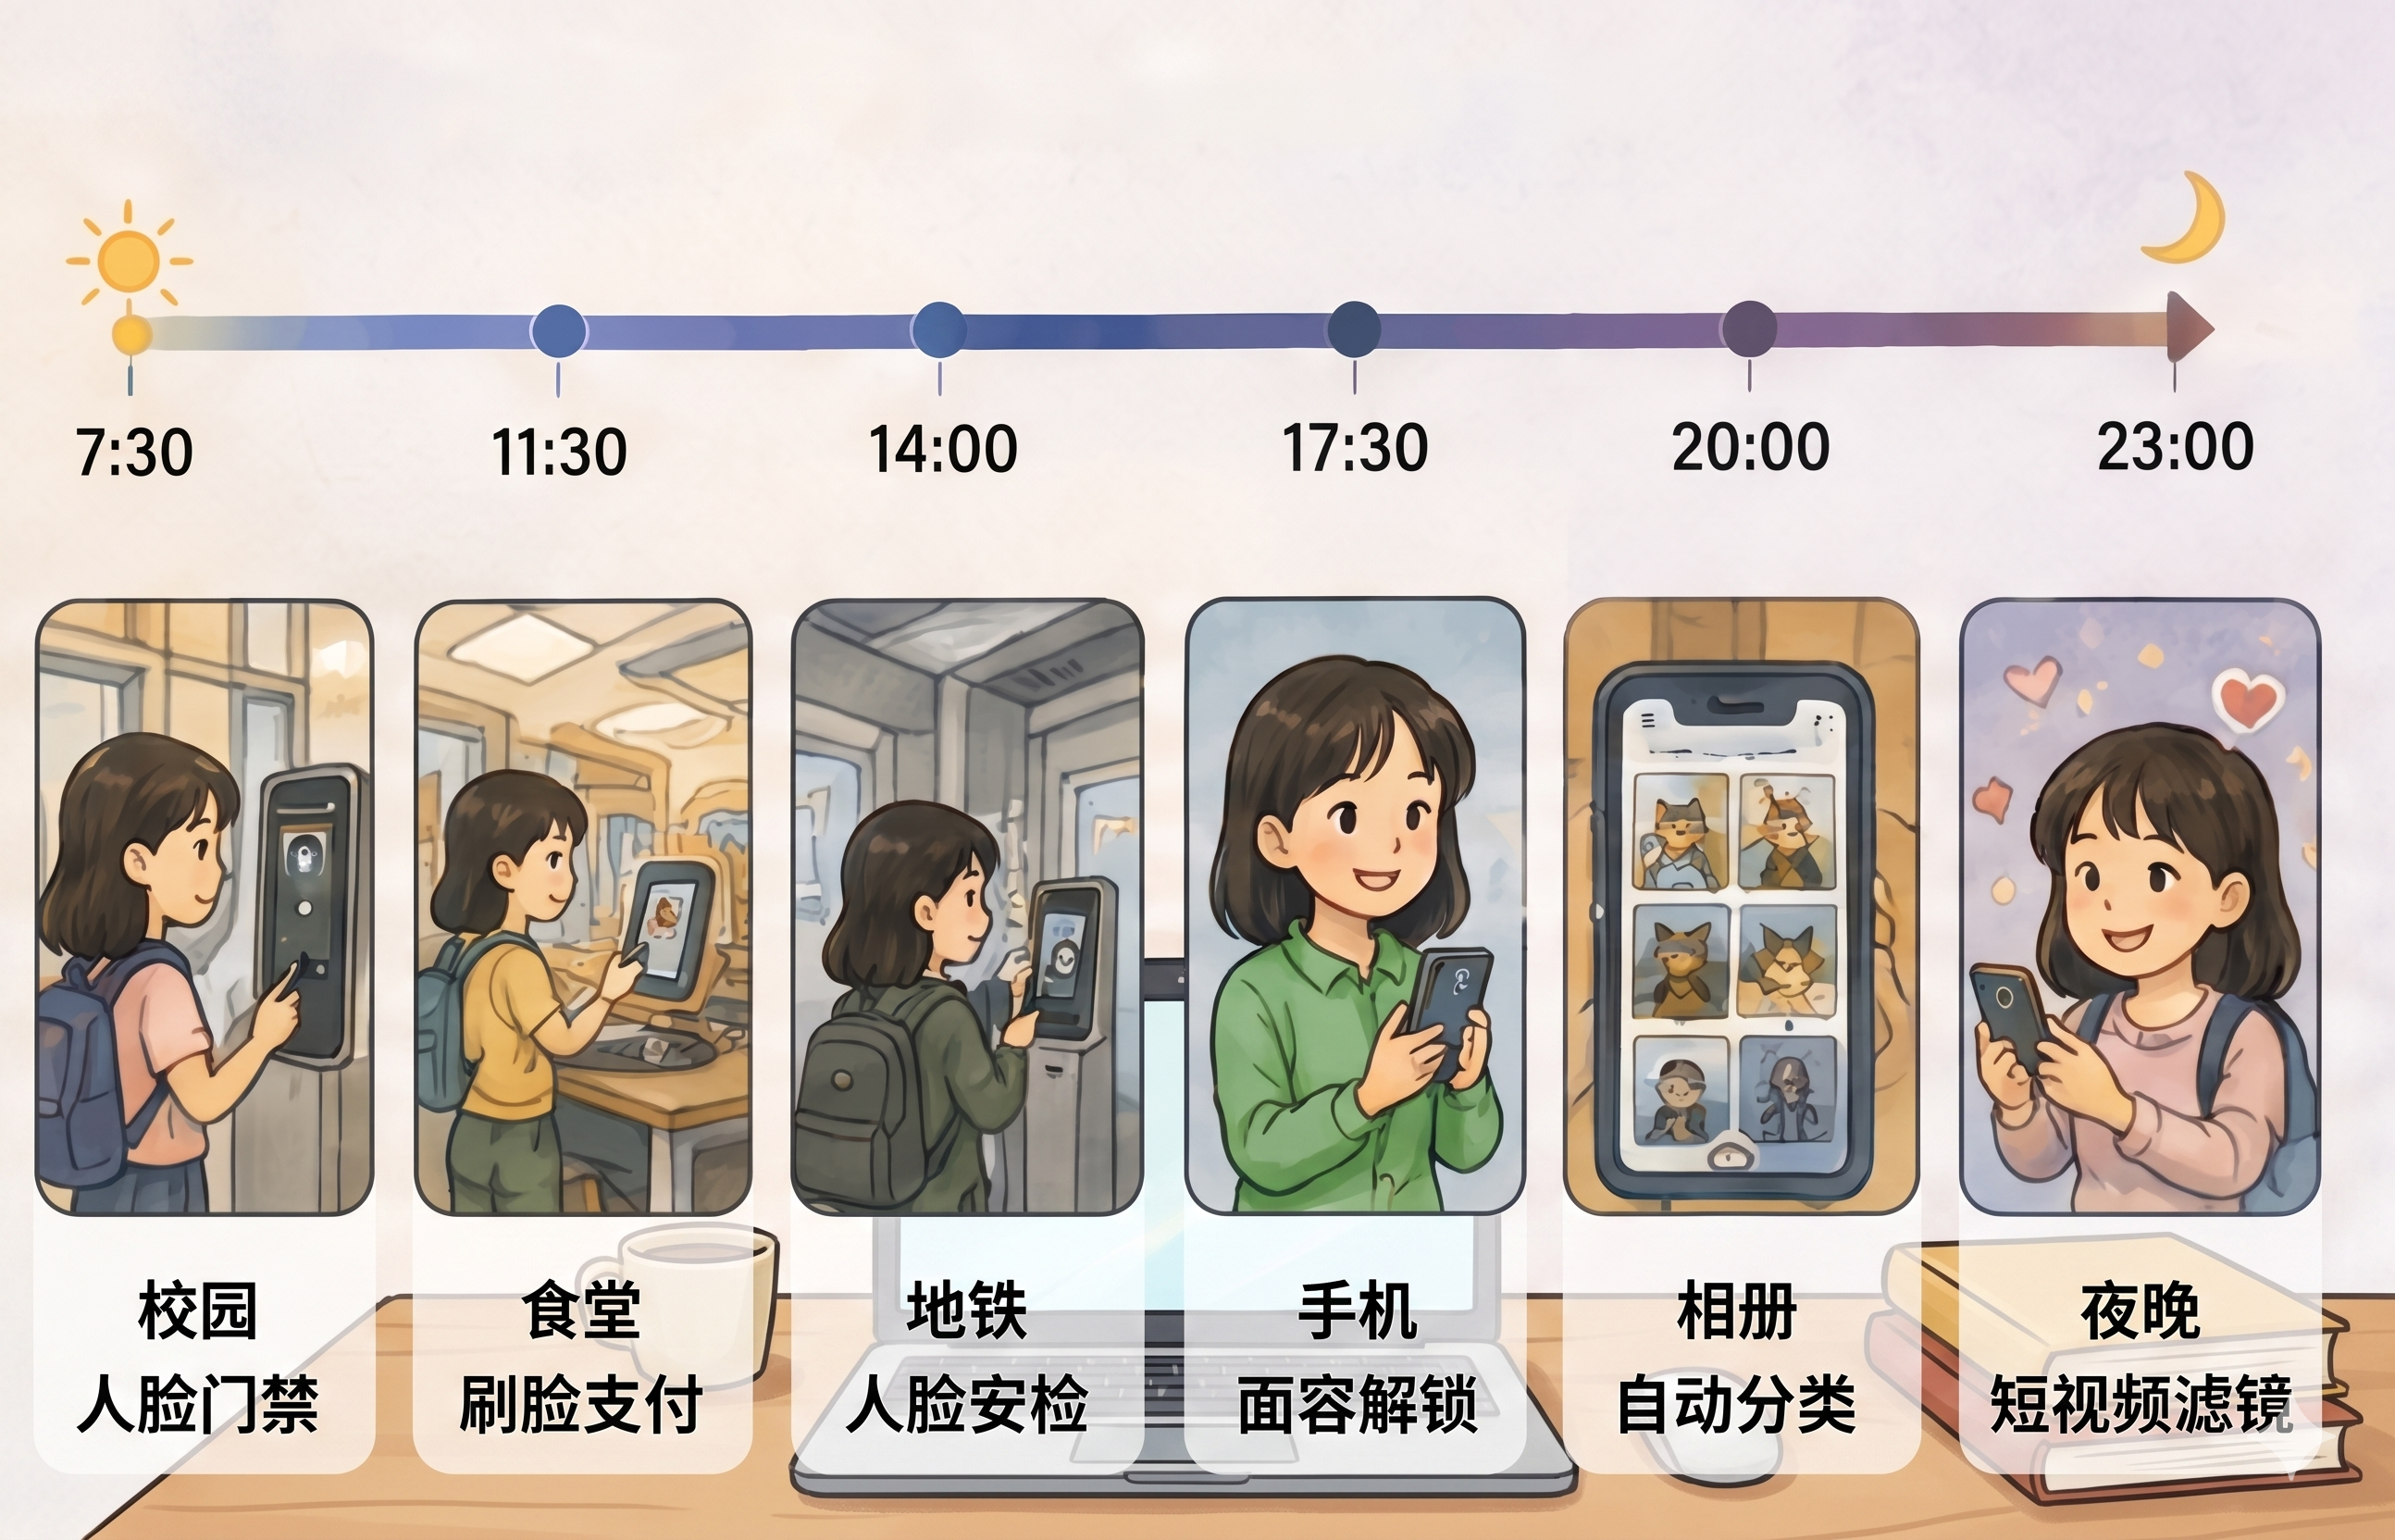
\includegraphics[width=0.88\textwidth]{images_chapter_01-03/2-6.png}
\caption*{\footnotesize\itshape\color{gray!50} 图2-2\quad 推荐系统如何从行为数据中“拼出”用户画像}
\end{figure}

了解了这些原理，我们来看看语言智能在现实生活中到底能做什么。

\subsection{语言智能应用案例}

语言智能正在从“单一任务的工具”变成“跨场景的通用助手”。在学习领域，它帮学生总结论文、整理笔记、辅导语言学习；在办公领域，它自动生成会议纪要、起草邮件、整理周报；在科研领域，它辅助文献检索、翻译外文论文、归纳研究趋势；在医疗领域，它帮医生语音录入病历、整理诊断报告；在娱乐领域，它写剧本、生成歌词、设计对话角色；在跨语言交流中，它让实时翻译从生硬逐字走向自然流畅。

下面，我们通过三个来自不同领域的案例，看看语言智能具体是如何运作的。

\subsubsection*{案例1：AI辅助阅读论文——从三小时到四十分钟}

研一新生小赵正坐在图书馆里，对着电脑屏幕上的一篇英文论文发愁。这是导师让他读的第一篇文献，发表在Nature上，关于蛋白质结构预测的最新研究。十几页正文加上几十条参考文献，光是摘要就有400多个单词，里面好几个专业术语他见都没见过。

过去，一个研究生面对这种情况的标准流程是：逐段翻译——遇到不认识的词查词典；看到专业术语去搜索含义；手动摘录重要段落到笔记本上；最后自己归纳核心观点、研究方法和主要发现。小赵的室友去年就是这么做的。“第一篇论文花了我三个下午，”室友说，“后来熟练了，一篇也要两三个小时。”

但现在，小赵把论文PDF上传到AI工具，输入了一句话：“请帮我总结这篇论文的核心观点，用表格呈现研究方法、主要发现和研究局限性。另外，用通俗的语言解释一下那些专业术语。”

大约二十多秒后，AI给出了回复。它先列了一张简洁的表格：研究方法是什么、主要发现是什么、局限性在哪里。接着，它把论文中像“homologous sequence alignment”“residue co-evolution”这样的专业术语用大白话解释了一遍——不是像词典那样冰冷地给出定义，而是结合论文上下文，告诉你“这个词在这篇论文里的意思是……”。

小赵后来回忆：“我当时的感觉就像——以前是你一个人在黑暗的隧道里摸索，现在突然有人递给你一个手电筒，还说‘这边我走过，跟着我’。”他当然没有把AI的输出照单全收。读完全文后他核对了AI的总结，发现基本准确，只有一个细节有些偏差。他用AI整理的知识框架作为骨架，自己填充了更多阅读后的理解和批判性思考。原本可能花三个小时的工作，变成了大约四十分钟——还包括了与AI来回讨论、追问细节的时间。

这个案例的核心启示是：大模型最大的变化不是“比搜索引擎搜得更准”，而是它从一个“只能做一件事的工具”变成了一个“能辅助整个工作流的助手”。AI不是替代研究者，而是让研究者把精力从繁琐的信息整理中解放出来，投入到更高层次的批判性思考中去。

\subsubsection*{案例2：AI翻译从“生硬逐字”走向“理解上下文”}

如果你用过十年前的翻译软件，应该还记得那种生硬感——每个单词都翻译了，但拼在一起完全不像人话。英文谚语“It's raining cats and dogs”曾有过“正在下雨猫和狗”的著名翻译，让读者一脸茫然。

今天的大模型翻译已经开始结合上下文做更自然的转换。当它读到“It's raining cats and dogs”时，它不只是查词典——它从海量中英文对照文本中学到了，这句话在中文里对应的习惯表达是“下着倾盆大雨”或“雨下得很大”。当它翻译一封商务邮件时，它会根据邮件的正式程度调整语气——不会把“Best regards”翻译成“最好的问候”，而是自然地翻译为“此致敬礼”或“祝好”。

更关键的是，大模型翻译能“理解”整个段落的意思，而不是一句一句孤立地翻。在一篇关于气候变化的英文报道中，同一个词“bank”可能在不同位置分别表示“银行”“河岸”“倾斜”。传统翻译软件可能翻错其中一两处，而大模型通过分析整段话的语境，能正确区分每个“bank”的含义。

一位留学生分享了他的体验：他用AI翻译工具阅读德文哲学论文。过去他需要借助词典逐句啃，现在他先让AI生成一个流畅的中文版本，然后对照原文精读，重点关注那些复杂的论证段落。翻译变成了辅助理解的工具，而不是替代品。

\begin{figure}[H]
\centering
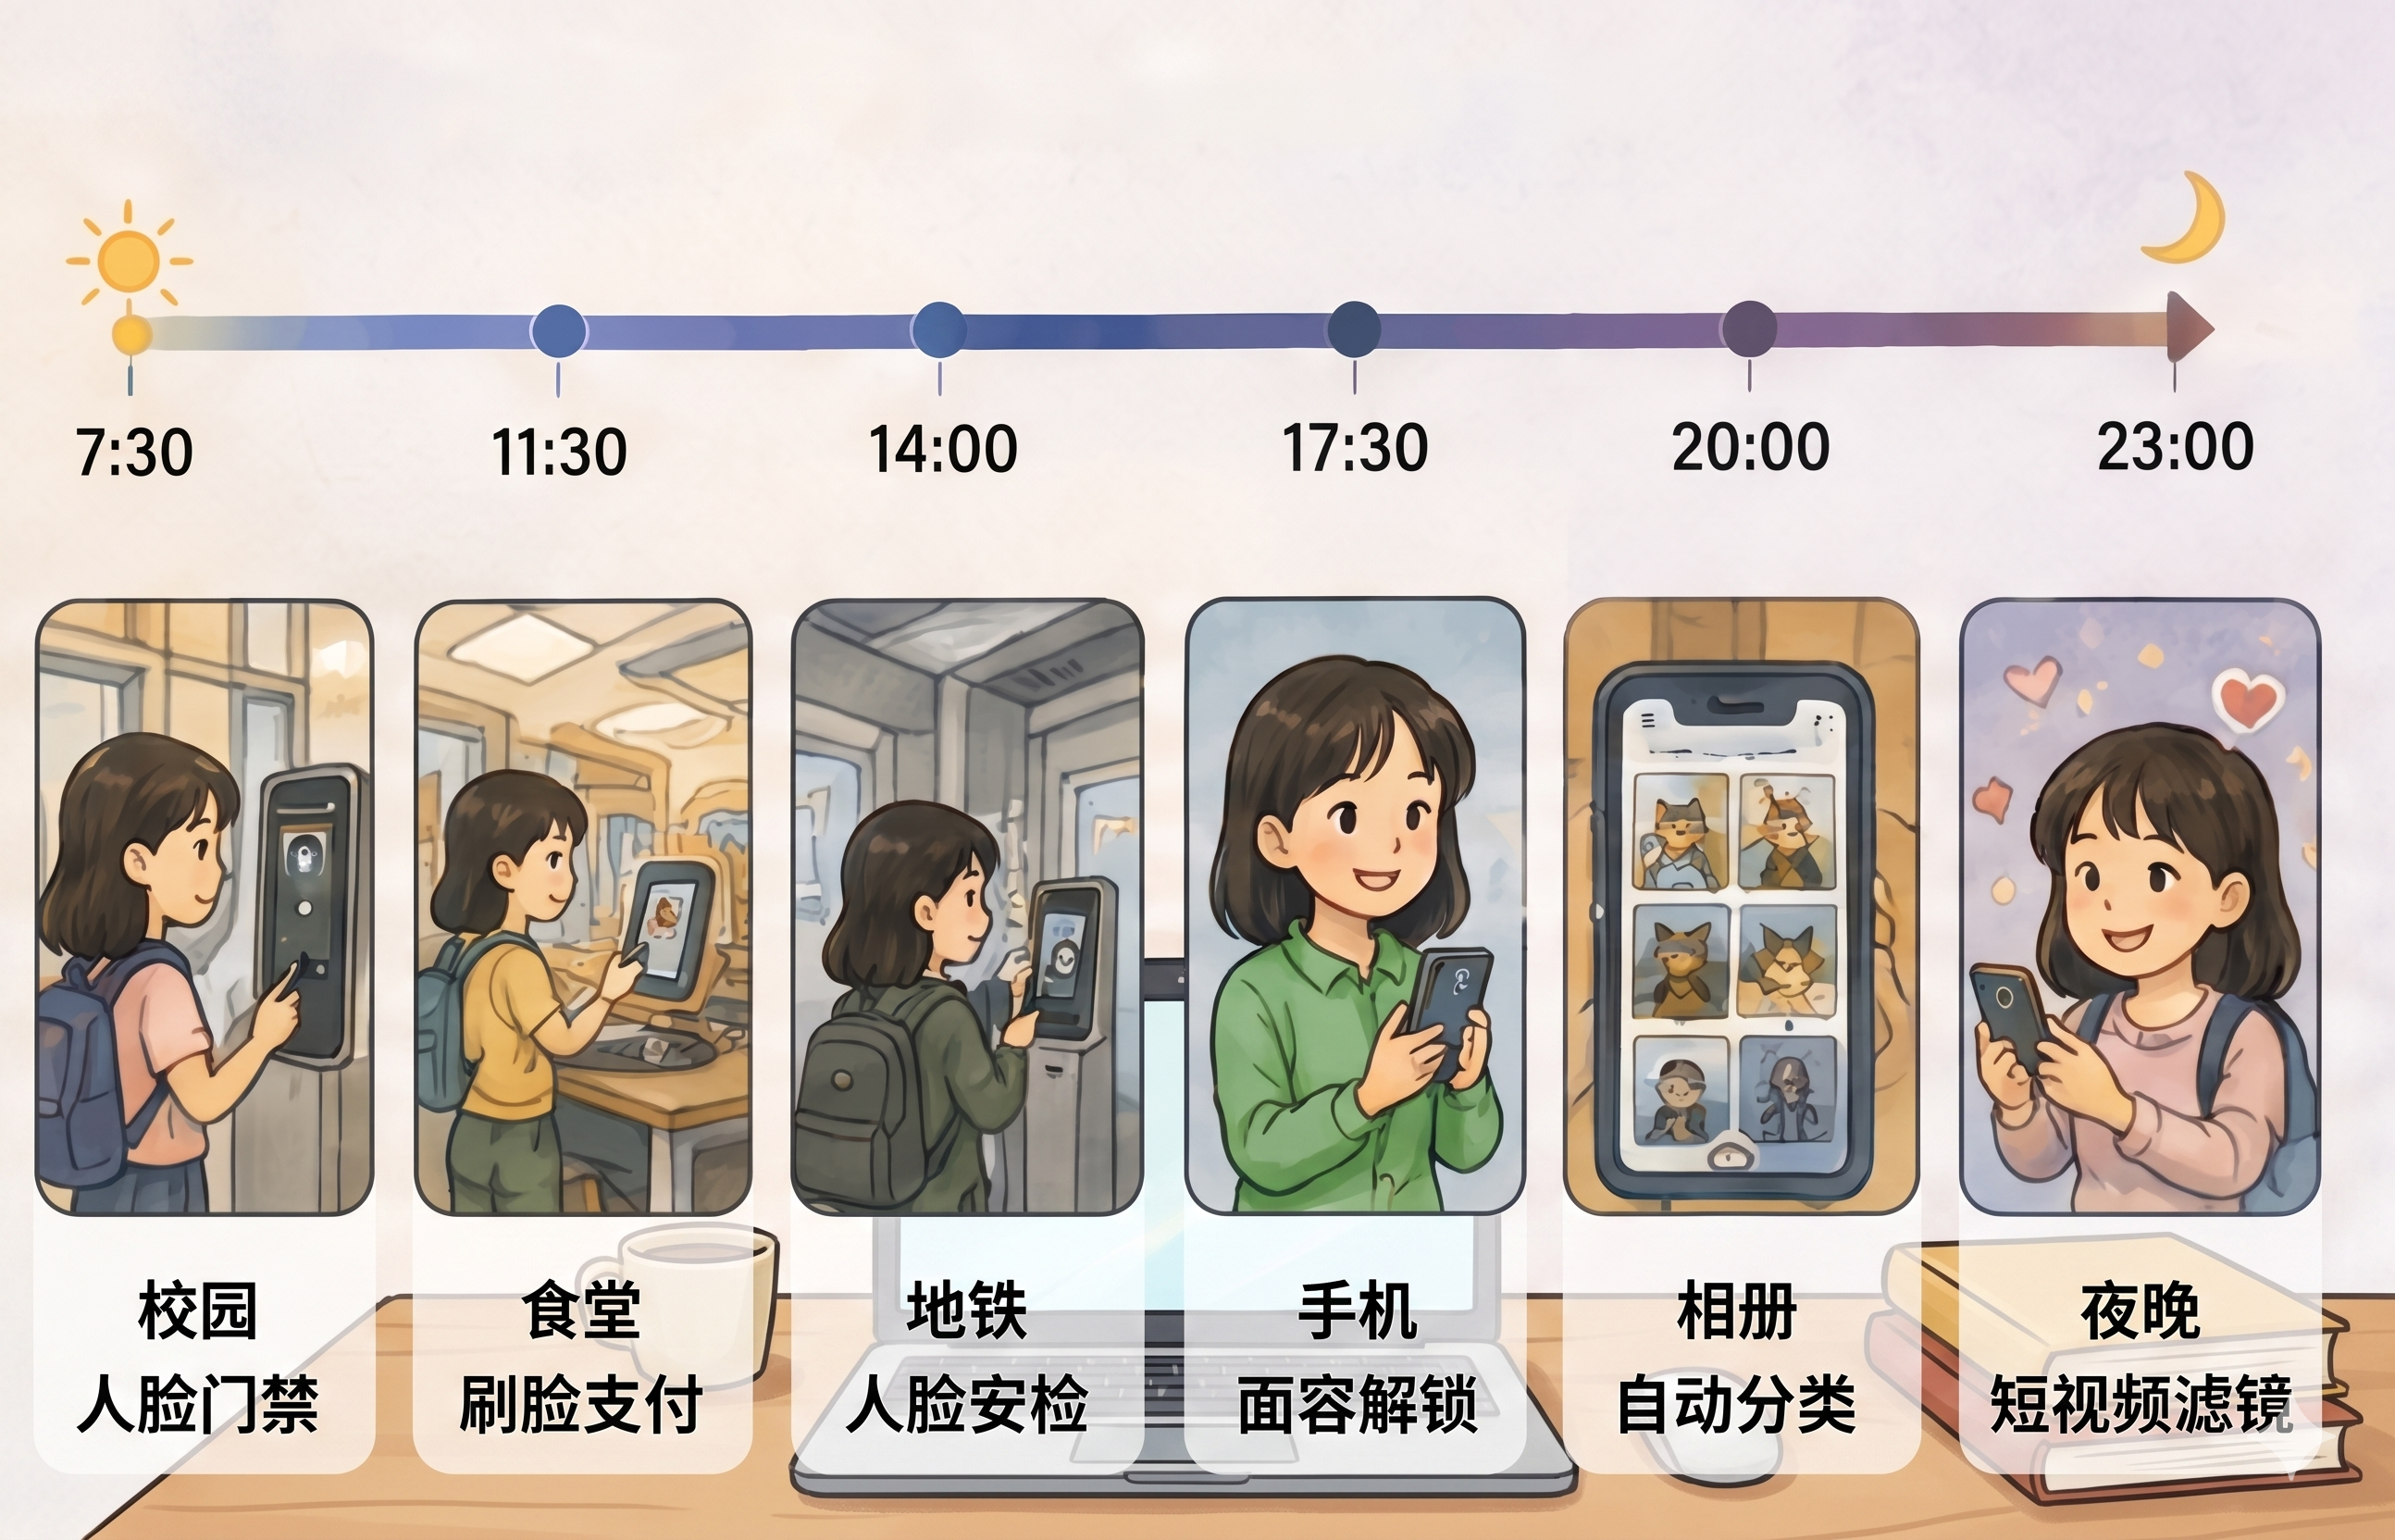
\includegraphics[width=0.88\textwidth]{images_chapter_01-03/2-6.png}
\caption*{\footnotesize\itshape\color{gray!50} 图2-2\quad 推荐系统如何从行为数据中“拼出”用户画像}
\end{figure}

\subsubsection*{案例3：AI语音助手从“执行指令”走向“自然对话”}

“嘿Siri，设一个明早7点的闹钟”——这是传统语音助手能做的事。它能理解关键词“闹钟”和“7点”，然后执行预设的指令。

但如果你说：“帮我查一下明天从北京到上海的高铁，要上午出发、3小时以内的车次，顺便看看上海明天的天气”——传统语音助手可能就糊涂了。这个请求里包含了多个任务（查高铁、筛选条件、查天气），而且任务是嵌套和关联的（先查高铁时间，再根据出发时间看天气）。

现在的大模型语音助手可以处理这样的复杂请求。它先理解整句话的意图——不是简单地识别关键词，而是理解“查高铁+筛选条件+顺便查天气”的完整任务结构。然后它调用火车票查询工具获取车次信息，按照“上午出发、3小时以内”的条件筛选，再调用天气工具查询上海明天的天气。最后把两个结果整合成一段自然的回复：“明天北京到上海上午出发且3小时以内的车次有G1次（9:00-12:28）和G3次（10:30-13:35）。顺便说一下，上海明天多云转阴，气温15-22℃，建议带一件薄外套。”

从“听懂关键词执行命令”到“理解整句话的意图并完成复杂查询”，语音助手正在越来越接近一个真正的“助手”。它不再只是“听懂指令”，而是开始“理解需求”。

\subsection{AI真的“理解”语言吗}

先讲一个真实故事。2023年，美国一位律师在准备一份诉讼材料时，使用了ChatGPT帮他检索相关判例。AI很快给出了六个判例，格式完整——有案件名称、审理法院、判决日期，甚至详细的案件编号。律师把这些内容写进了法律文书，提交给法庭。结果，对方律师在核查时发现：\textbf{这六个判例，一个都不存在。} AI完全编造了它们。

这个故事揭示了一个核心问题：\textbf{AI擅长的是“生成看起来合理的语言”，而不是“陈述事实”。} 用技术术语来说，这叫\textbf{AI幻觉}（Hallucination）——AI在生成内容时，并不知道什么是真、什么是假。它只是在做概率计算：基于你给的提示词，什么词接在后面最合理？如果训练数据中对某个问题没有足够的信息，AI就可能“杜撰”——但它不会告诉你“我不知道”，它会编造一个看起来像真的答案。

\begin{knowledgebox}
\textbf{AI幻觉——一个超级模仿演员的即兴表演}

\textbf{AI幻觉}是指AI生成的内容虽然表达流畅、看起来合理，但包含事实性错误或完全虚构的信息。可以这样理解：AI像一个超级模仿演员，看了无数部法庭电影，学会了律师说话的方式。你让他即兴来一段“律师在法庭上的慷慨陈词”——语气、用词、逻辑都无可挑剔。但他说的每一个案号、每一条法条，都是根据“应该这样演”而编出来的。AI就是这位演员。它没有被设计成“诚实”，而是被设计成“继续接龙”。这解释了为什么它能在法庭上“义正词严”地引用根本不存在的判例。
\end{knowledgebox}

类似的故事还有很多：有人让AI推荐旅游攻略，AI推荐了一个根本不存在的景点；有人让AI解释一道物理题，AI条理清晰地给出了错误答案；有人和AI聊得投机，但发现AI完全理解不了讽刺和隐喻——你说“今天真是个好日子”（其实你在反讽，因为出门就被雨淋了），AI会认真地回复你：“是的，晴天总是让人心情愉快。”

所以，回到本节的核心问题：\textbf{AI真的“理解”语言吗？}

答案很明确：\textbf{不，它不理解。} AI是一个超级模仿者。它读过人类写过的几乎所有东西，学会了人类使用语言的各种模式。它能生成优美、流畅、看似有理有据的回答。但它对自己输出的内容没有“真伪判断”。它不知道自己是在陈述事实还是在编造故事。它可以在几秒钟内写出一篇论文，但不知道那篇论文的质量和真实性。它可以回复你“我理解你的感受”——但它没有感受过任何东西。它不理解悲伤，不理解孤独，不理解爱。

今天的大模型确实让AI的语言能力产生了飞跃。它能辅助学习、办公、创作，效率惊人。但它仍然是工具，不是拥有意识的人类。它输出的一切内容，都需要人类判断是否真实、是否合适、是否可用。真正重要的，不是“AI越来越像人了”，而是我们如何学会正确地使用它，并始终保持独立思考和批判性判断。

\section{生成式AI：机器也能“创造”内容}

2022年8月，美国科罗拉多州。游戏设计师杰森·艾伦（Jason Allen）坐在电脑前，反复修改着输入一段文字描述。他在Midjourney中不断调整提示词，尝试了上百个版本。最终，他选择了一幅作品参赛。这幅画名为《太空歌剧院》（Théâtre d'Opéra Spatial）——一个恢弘的巴洛克式舞台上，身着华丽戏服的演员们沐浴在金色光束中，背景是深邃的星空和巨大的行星。评委将数字艺术类别的最高奖项颁给了它。

然后事情就炸了。媒体蜂拥而至，艺术界分裂为两个阵营。一方说这是作弊——“AI生成的画不应该被称为艺术”。另一方说这是新时代的开端——“就像摄影没有杀死绘画，AI也不会杀死艺术”。杰森·艾伦本人在接受采访时说了一句意味深长的话：“我不是画家，我赢了比赛。我提交的不是一幅画，而是一个声明。”一个什么声明？一个关于“创造力”正在被重新定义的声明。

\subsection{当AI开始画画、写文章、做音乐}

大一学生小陈是校学生会宣传部的干事。新学期开学，他接到一个任务：三天之内设计一张招新海报。他不会用Photoshop，更没学过设计。在过去，他只能求助设计专业的学长或者从网上下载模板来改——结果往往是“改来改去还是像模板”。

但这一次，他打开了一款AI绘图工具。他花了几分钟想清楚自己需要什么，然后输入：“一张现代风格的学生会招新海报。背景是校园标志性建筑的线条简化图，前景是几个抽象的大学生在热烈讨论，配色以校徽的深蓝色为主调、点缀明亮的橙色。画面底部留白，用于放置招新信息和二维码。”

几十秒后，AI生成了四张不同设计风格的海报供他挑选。小陈选了一张最能体现“活力”的，用AI的局部重绘功能把背景中的建筑线条调得更简洁，然后在底部预留的空白处手动加上了招新群二维码。从构思到成品，不到四十分钟。

他把海报发到学生会群里，一位大三的设计专业学姐在群里问：“这次是谁做的？构图挺干净的。”小陈回了一句：“我提的想法，AI执行的。”群里安静了几秒。然后学姐回了一句：“……好吧，看来我也得学学怎么用AI了。”

不只是海报。在宿舍另一边，一位中文系的同学正在用AI润色小说创作的语言。一位计算机系的学生用AI生成了一段原创旋律，准备用在校园微电影的配乐上。过去，这些创作行为各自有着高高的门槛——你要会画画、会写文章、会编曲、会设计。而现在，门槛正在被AI系统性地降低。

你可能会问：\textbf{AI为什么突然“会创作”了？就在几年前，它还只会“认猫认狗”。这个转变是怎么发生的？}

\subsection{AI没有灵感，为什么“创作”的还挺像样}

要回答这个问题，我们得先搞清楚：\textbf{人类是怎么创作的？AI又是怎么“创作”的？}

人类创作一首情歌，可能是因为刚经历了一场刻骨铭心的恋爱。他坐在钢琴前，想起某个人、某个场景、某个瞬间，心里涌出的情感变成了旋律。

AI呢？AI没有恋爱过，没有被分手过，没有在深夜辗转反侧过。但它“听”过数以万计的人类情歌。它分析了无数情歌的旋律走向、和弦进行、歌词节奏——它从中总结出了“情歌通常是这样写的”的规律。当你让它创作一首情歌时，它把那些规律重新组合，生成了一首“听起来像情歌”的歌。

一个很好的类比：一个学生，没去过巴黎，没谈过恋爱，没经历过人生的大起大落。但他临摹过一万张梵高的画。慢慢地，他不仅能画出和梵高原作几乎一模一样的画，还能画梵高没有画过的题材——比如把埃菲尔铁塔画成梵高《星月夜》的风格。他画的不是巴黎，也不是他自己，而是“如果梵高画巴黎，大概会这么画”。

生成式AI就是那个学生。它没有灵感，没有情感，没有生活。但它有几十亿张画作、几亿篇文章、几千万首音乐的训练样本。

\textbf{核心认知}：生成式AI的“创作”，本质不是“表达”，而是\textbf{模仿重组}。它分析海量作品的风格规律，然后根据你的要求，重新组合出一个“看起来像人类作品”的新内容。它不是从无到有地创造，而是在对已有模式进行超大规模的“拼合和变奏”。

\subsection{生成式AI——当AI学会“举一反三”}

先区分两个概念：\textbf{传统判别式AI vs 生成式AI}。

传统AI（也叫判别式AI）的核心能力是“判断”——给它一张照片，它判断这是猫还是狗。给它一封邮件，它判断这是正常邮件还是垃圾邮件。它像一个鉴定师。生成式AI的核心能力是“创造”——给它一行文字描述，它能画出一张全新的画。给它一段提示，它能写出一篇原创文章。它更像一个创作者。

\begin{figure}[H]
\centering
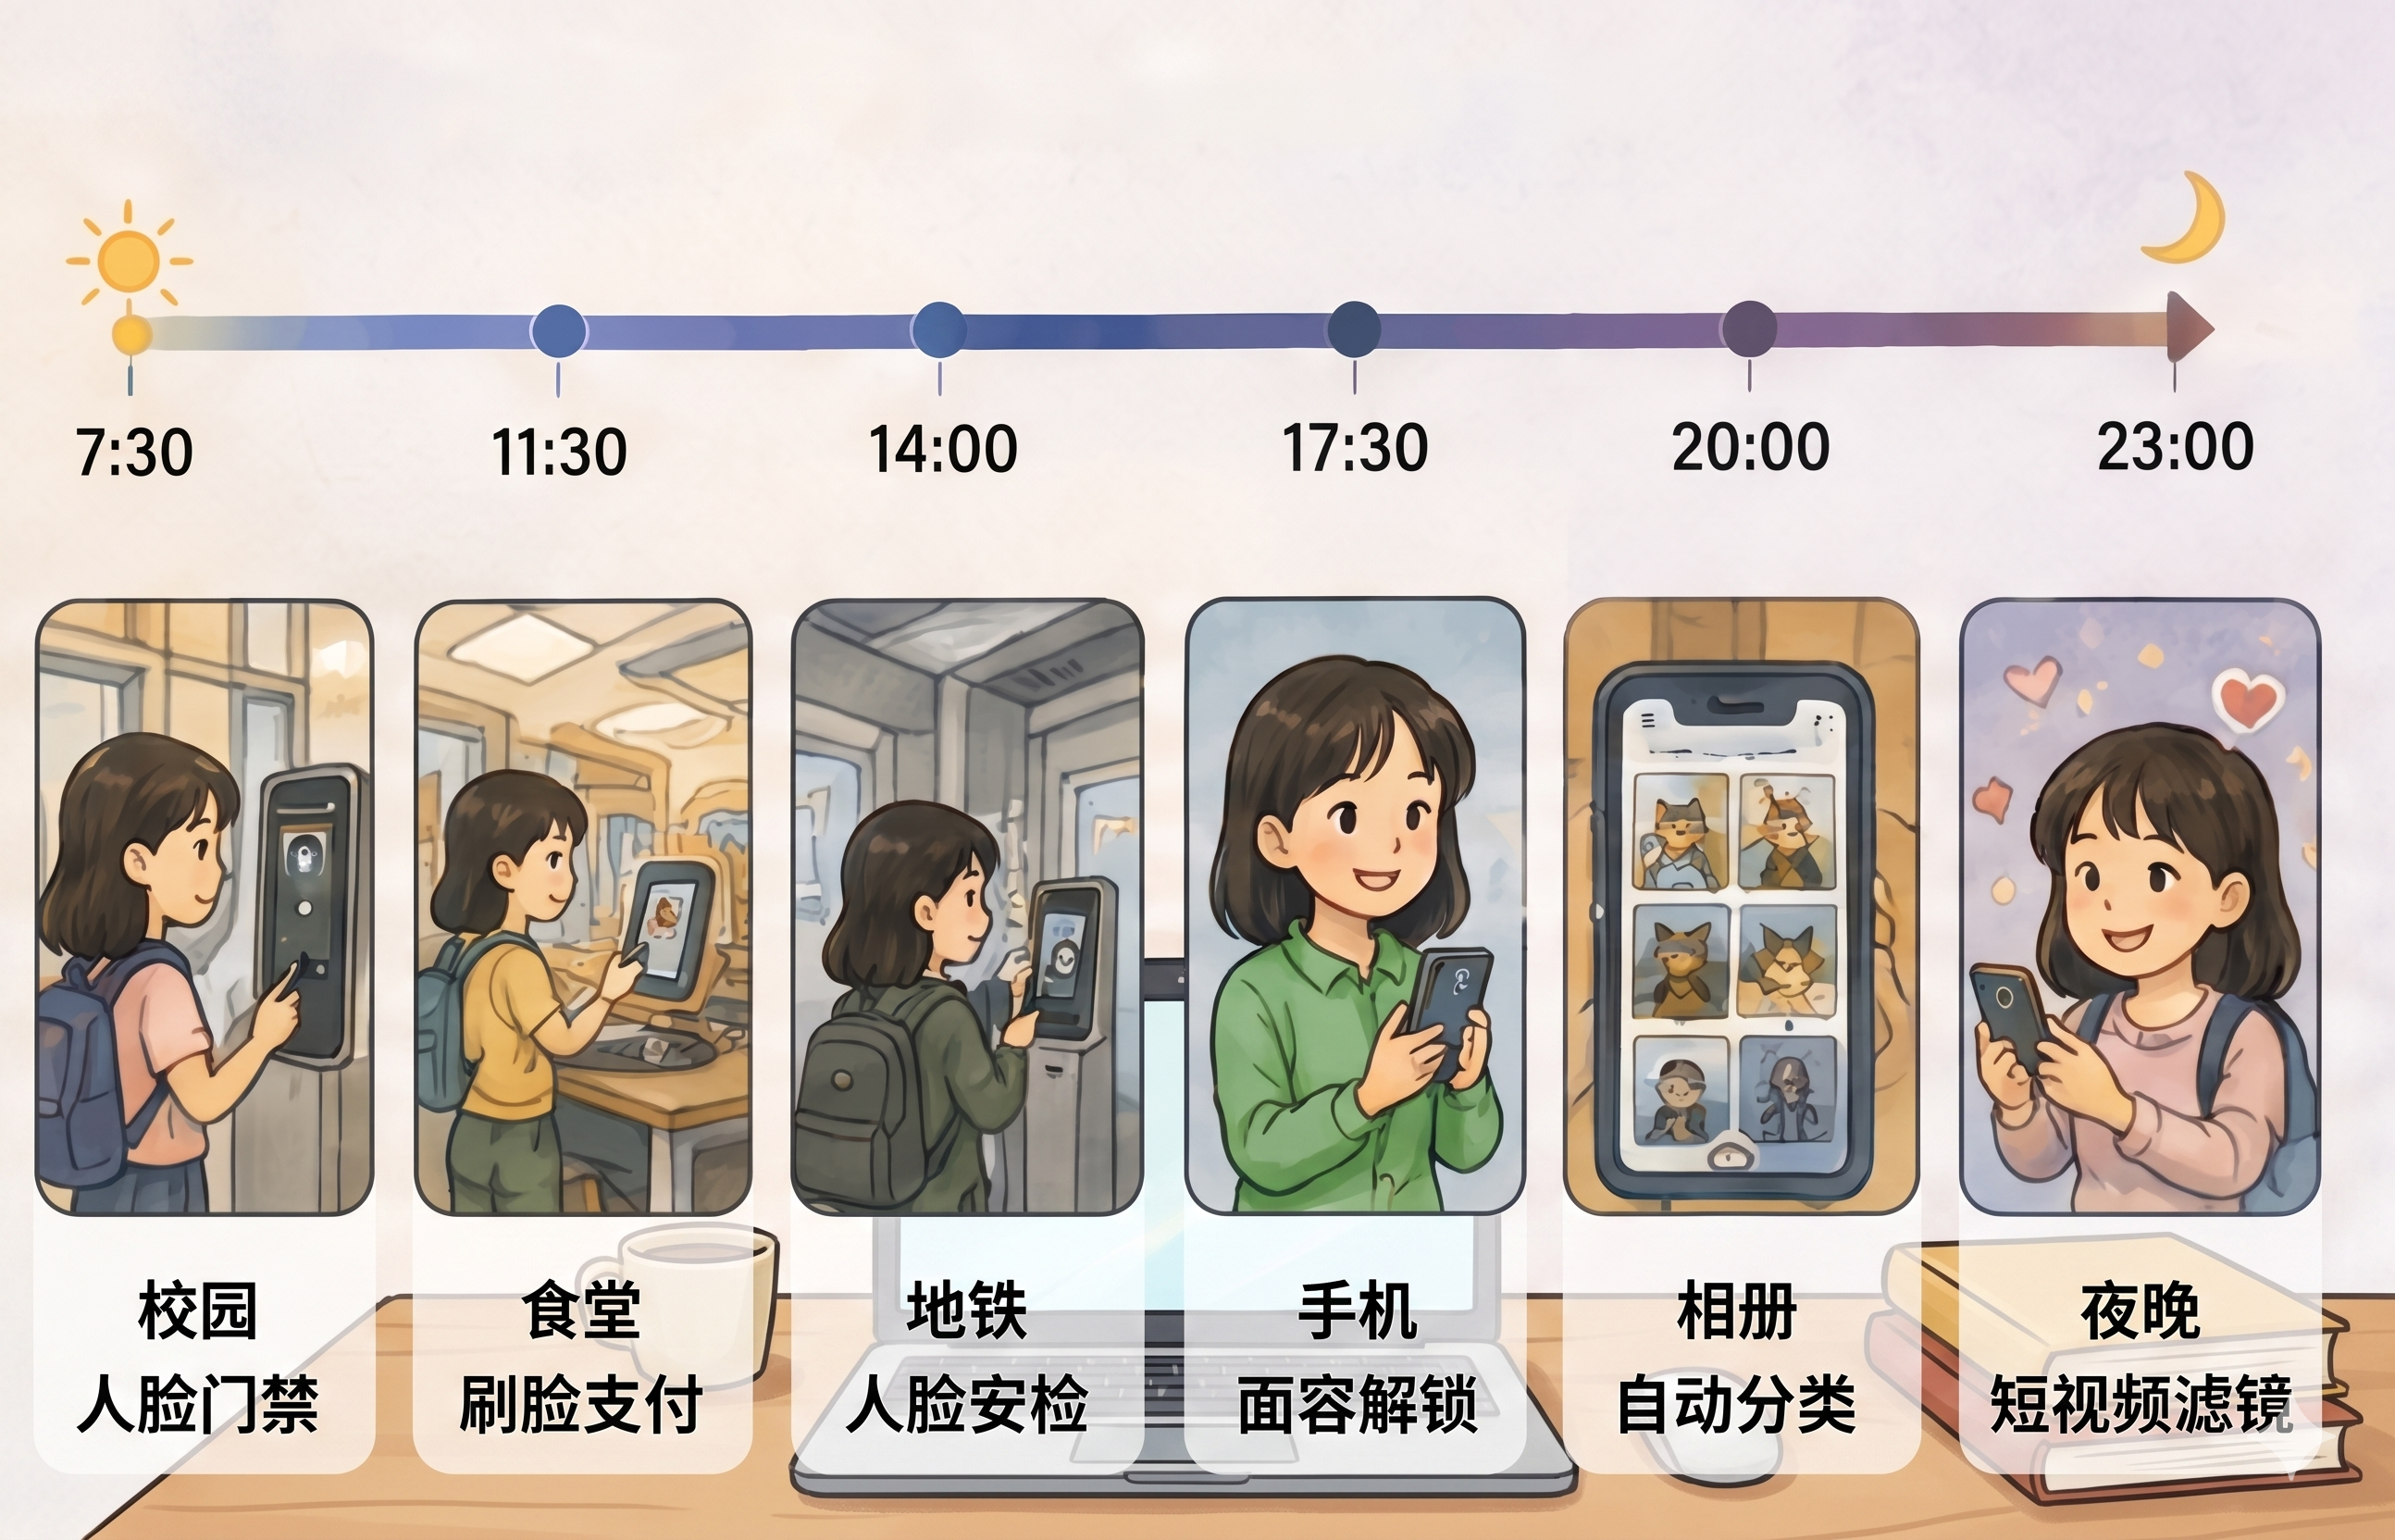
\includegraphics[width=0.88\textwidth]{images_chapter_01-03/2-6.png}
\caption*{\footnotesize\itshape\color{gray!50} 图2-2\quad 推荐系统如何从行为数据中“拼出”用户画像}
\end{figure}

\textbf{生成式AI是怎么“学”的？} 用学书法来类比最好理解。你先是临摹王羲之的字帖，一笔一画模仿他的笔锋。临摹了几百遍几千遍之后，你不仅能把王羲之的字写得很像，还能写王羲之没有写过的字——“鸑”“鷟”这些生僻字王羲之可能没写过，但你写的看起来就像他的笔迹。生成式AI就是那个临摹过几千万张作品的学生。它不是“学会了王羲之的书法”，而是“学会了王羲之写字的统计模式”。

\begin{knowledgebox}
\textbf{扩散模型与GAN——雕塑家与伪造者}

目前AI绘画工具（如Midjourney、Stable Diffusion）背后的核心技术，叫\textbf{扩散模型}。它的思想很巧妙：先给一张照片不断加噪点，直到它变成一片灰色雪花；然后训练AI反着来——从灰色雪花中一层层“去噪”，逐渐还原出清晰的图像。可以把它想象成一位雕塑家，从一块杂乱的石头中逐渐“雕出”清晰的形象。

而\textbf{生成对抗网络（GAN）}则是另一种思路：让两个AI互相“博弈”——一个负责伪造图像，一个负责鉴别真伪。通过数万轮对抗，伪造者最终学会了创作足以乱真的图像，就像一个在一次次被识破中手艺日臻精湛的伪造大师。Deepfake换脸技术就是基于GAN。
\end{knowledgebox}

\textbf{为什么这几年突然爆发？} 三个词：数据、算力、算法。数据——互联网几十年的积累，给了AI几十亿张图片、几万亿字的文本用来“临摹”。算力——GPU等高性能芯片让训练超大模型成为可能。算法——扩散模型、Transformer等新架构让AI终于能高效处理海量数据并提取复杂规律。三个要素同时突破，量变引起质变。

\subsection{生成式AI应用案例}

生成式AI正在让“创作”从少数经过专业训练的人的专属，变成每个有想法的人都可以尝试的事。在设计领域，它快速生成海报、Logo和UI设计方案；在写作领域，它辅助构思大纲、润色语言、生成创意文案；在影视领域，它辅助编剧构思剧情、生成分镜参考图；在音乐领域，它生成旋律框架和伴奏；在文物保护领域，它根据残存数据复原历史文物的原貌；在教育领域，它生成习题、设计课件插图、制作教学视频素材。

下面，我们通过三个来自不同领域的案例，看看生成式AI具体是如何落地应用的。

\subsubsection*{案例1：AI辅助校园短剧编剧——从一个月到一周}

大四学生林语是校园话剧社的编剧。上学期她接到一个任务：为即将到来的校庆创作一部15分钟的短剧，主题是“百年来校园生活的变迁”。

按照传统流程，她需要查校史资料——至少翻阅几十篇文献、老照片集和校友回忆录；构思人物和剧情——要覆盖不同年代，得设计至少三组人物；写剧本——每一幕的对白、动作、舞台提示都要一个字一个字敲出来；修改——初稿出来后至少还要改五六版。整个流程下来，一个月非常紧张。

林语尝试了一个不一样的工作方式。她先是花了半天时间在校史馆和数字档案馆搜集资料，筛选出几个最具代表性的年代切片：抗战时期的西迁岁月、改革开放后的校园复苏、新世纪的信息化浪潮。然后，她将这些资料整理成一份“创作简报”，上传到AI工具。

她输入的指令是：“请根据这份校史资料，为一部15分钟的三幕短剧设计人物关系和剧情框架。三幕分别对应抗战时期、改革开放初期、信息时代。每一幕的时代细节要准确（服装、语言习惯、校园建筑），用表格呈现。”

AI很快给出了结构清晰的框架。更重要的是，它自动补充了林语自己可能花更长时间才能查到的细节——比如抗战时期女生校服的具体样式、80年代校园广播站常用的开场曲。林语在AI框架基础上，用了一天时间打磨对话和动作细节，三天后拿出了完整剧本。

“我不是被AI替代了，”林语后来在剧社分享会上说，“我是被AI加速了。以前一个月做的事，现在一周做完。省下的时间我用来和演员们排练、打磨表演——那些才是AI做不了的。”这个案例的核心启示是：生成式AI的真正价值，不是替代创作者，而是把创作者的精力从繁琐的前期工作中解放出来，投入到真正需要人类判断力、情感和审美的高价值环节中去。

\subsubsection*{案例2：AI帮文物“重现光彩”}

2024年，三星堆博物馆的文物保护团队与AI研究者合作，尝试用生成式AI复原那些残缺严重的出土文物。

以著名的青铜大立人像为例。这尊距今约三千年的青铜像出土时双手缺失，考古学界对手势有多种推测——是持笏？持象牙？持蛇？还是在做一个特定的祭祀手势？各种说法都有文献和同期文物作为依据，但没有人能确定。

AI团队的做法是：让AI学习商周时期同时代青铜器上所有人像手势的造型特征和纹饰规律。在“消化”了大量同时期文物数据后，AI根据铜像手腕的残断面形态和手臂角度，生成了几种不同手势的复原方案。它不提供“唯一正确答案”，而是给考古学家提供更直观的视觉讨论素材。考古团队可以根据每种方案评估其合理性和可能性，缩小推测范围。

另一个更贴近日常的案例是兵马俑的色彩复原。秦始皇陵兵马俑出土时，表面的彩绘层在接触空气后迅速氧化剥落，我们现在看到的陶俑是灰色的。但通过分析残存颜料的化学成分和矿物来源，结合同时期其他出土文物中保存较好的彩绘样本，AI可以生成“刚出土时”兵马俑的色彩复原图——那种两千年前鲜艳生动的彩绘冲击，是任何文字描述都难以传达的。

\subsubsection*{案例3：AI如何帮“数据恐惧症”的文科生做图表}

大二社会学专业学生小徐正在进行一项问卷调查，研究不同年级学生的短视频使用习惯。她回收了三百多份有效问卷，Excel里堆满了原始数据。指导老师要求她在报告里加入数据可视化图表——“至少要有柱状图和饼图”。小徐看到密密麻麻的数字，头都大了。

她对室友抱怨：“我一个文科生，哪会做什么数据透视表啊。”

室友给她推荐了一款AI数据工具。小徐把原始表格上传，在对话框里输入：“请根据这份问卷数据，生成一个对比柱状图，展示不同年级学生每周刷短视频的平均时长，用不同颜色区分年级，标注具体数值。图表标题为‘各年级学生短视频使用时长对比’。”

几十秒后，AI不仅生成了图表，还自动输出了一段文字分析：“大三学生周均短视频使用时长最高（14.2小时），大一最低（9.7小时），整体呈随年级递增趋势。可能原因：随着年级升高，课程压力减轻，可自由支配时间增多。”

小徐看完分析后，又追问了一句：“能帮我再做一个饼图吗？展示每天刷短视频的时段分布——上午、下午、晚上、深夜各占多少比例。”几秒后，第二张图表也完成了。

“原来不是数据分析难，”小徐后来在朋友圈写道，“是我一直用错了工具。AI不是替我做研究，而是帮我把数据‘翻译’成了图表。”这个案例的启示是：生成式AI正在降低专业工具的入门门槛，让更多人能把自己的想法可视化地表达出来。创作者需要的是清晰的表达力和判断力，而不是记住某个软件复杂的操作步骤。

\subsection{AI会取代人类创作者吗}

先看几个翻车现场。你用AI绘图工具画过“手”吗？大概率遇到过“六根手指”或“关节扭曲”的问题。这是著名的老毛病——因为训练数据中手的角度、姿态变化太多，AI很难完全掌握。你读过AI写的诗吗？语句优美，意象丰富，但读完之后总觉得少了点什么。少了什么呢？少了“有人真的经历过这一切”的真实感。AI可以写“我想你就像风走了八千里”，但它从没想过任何人。

\begin{figure}[H]
\centering
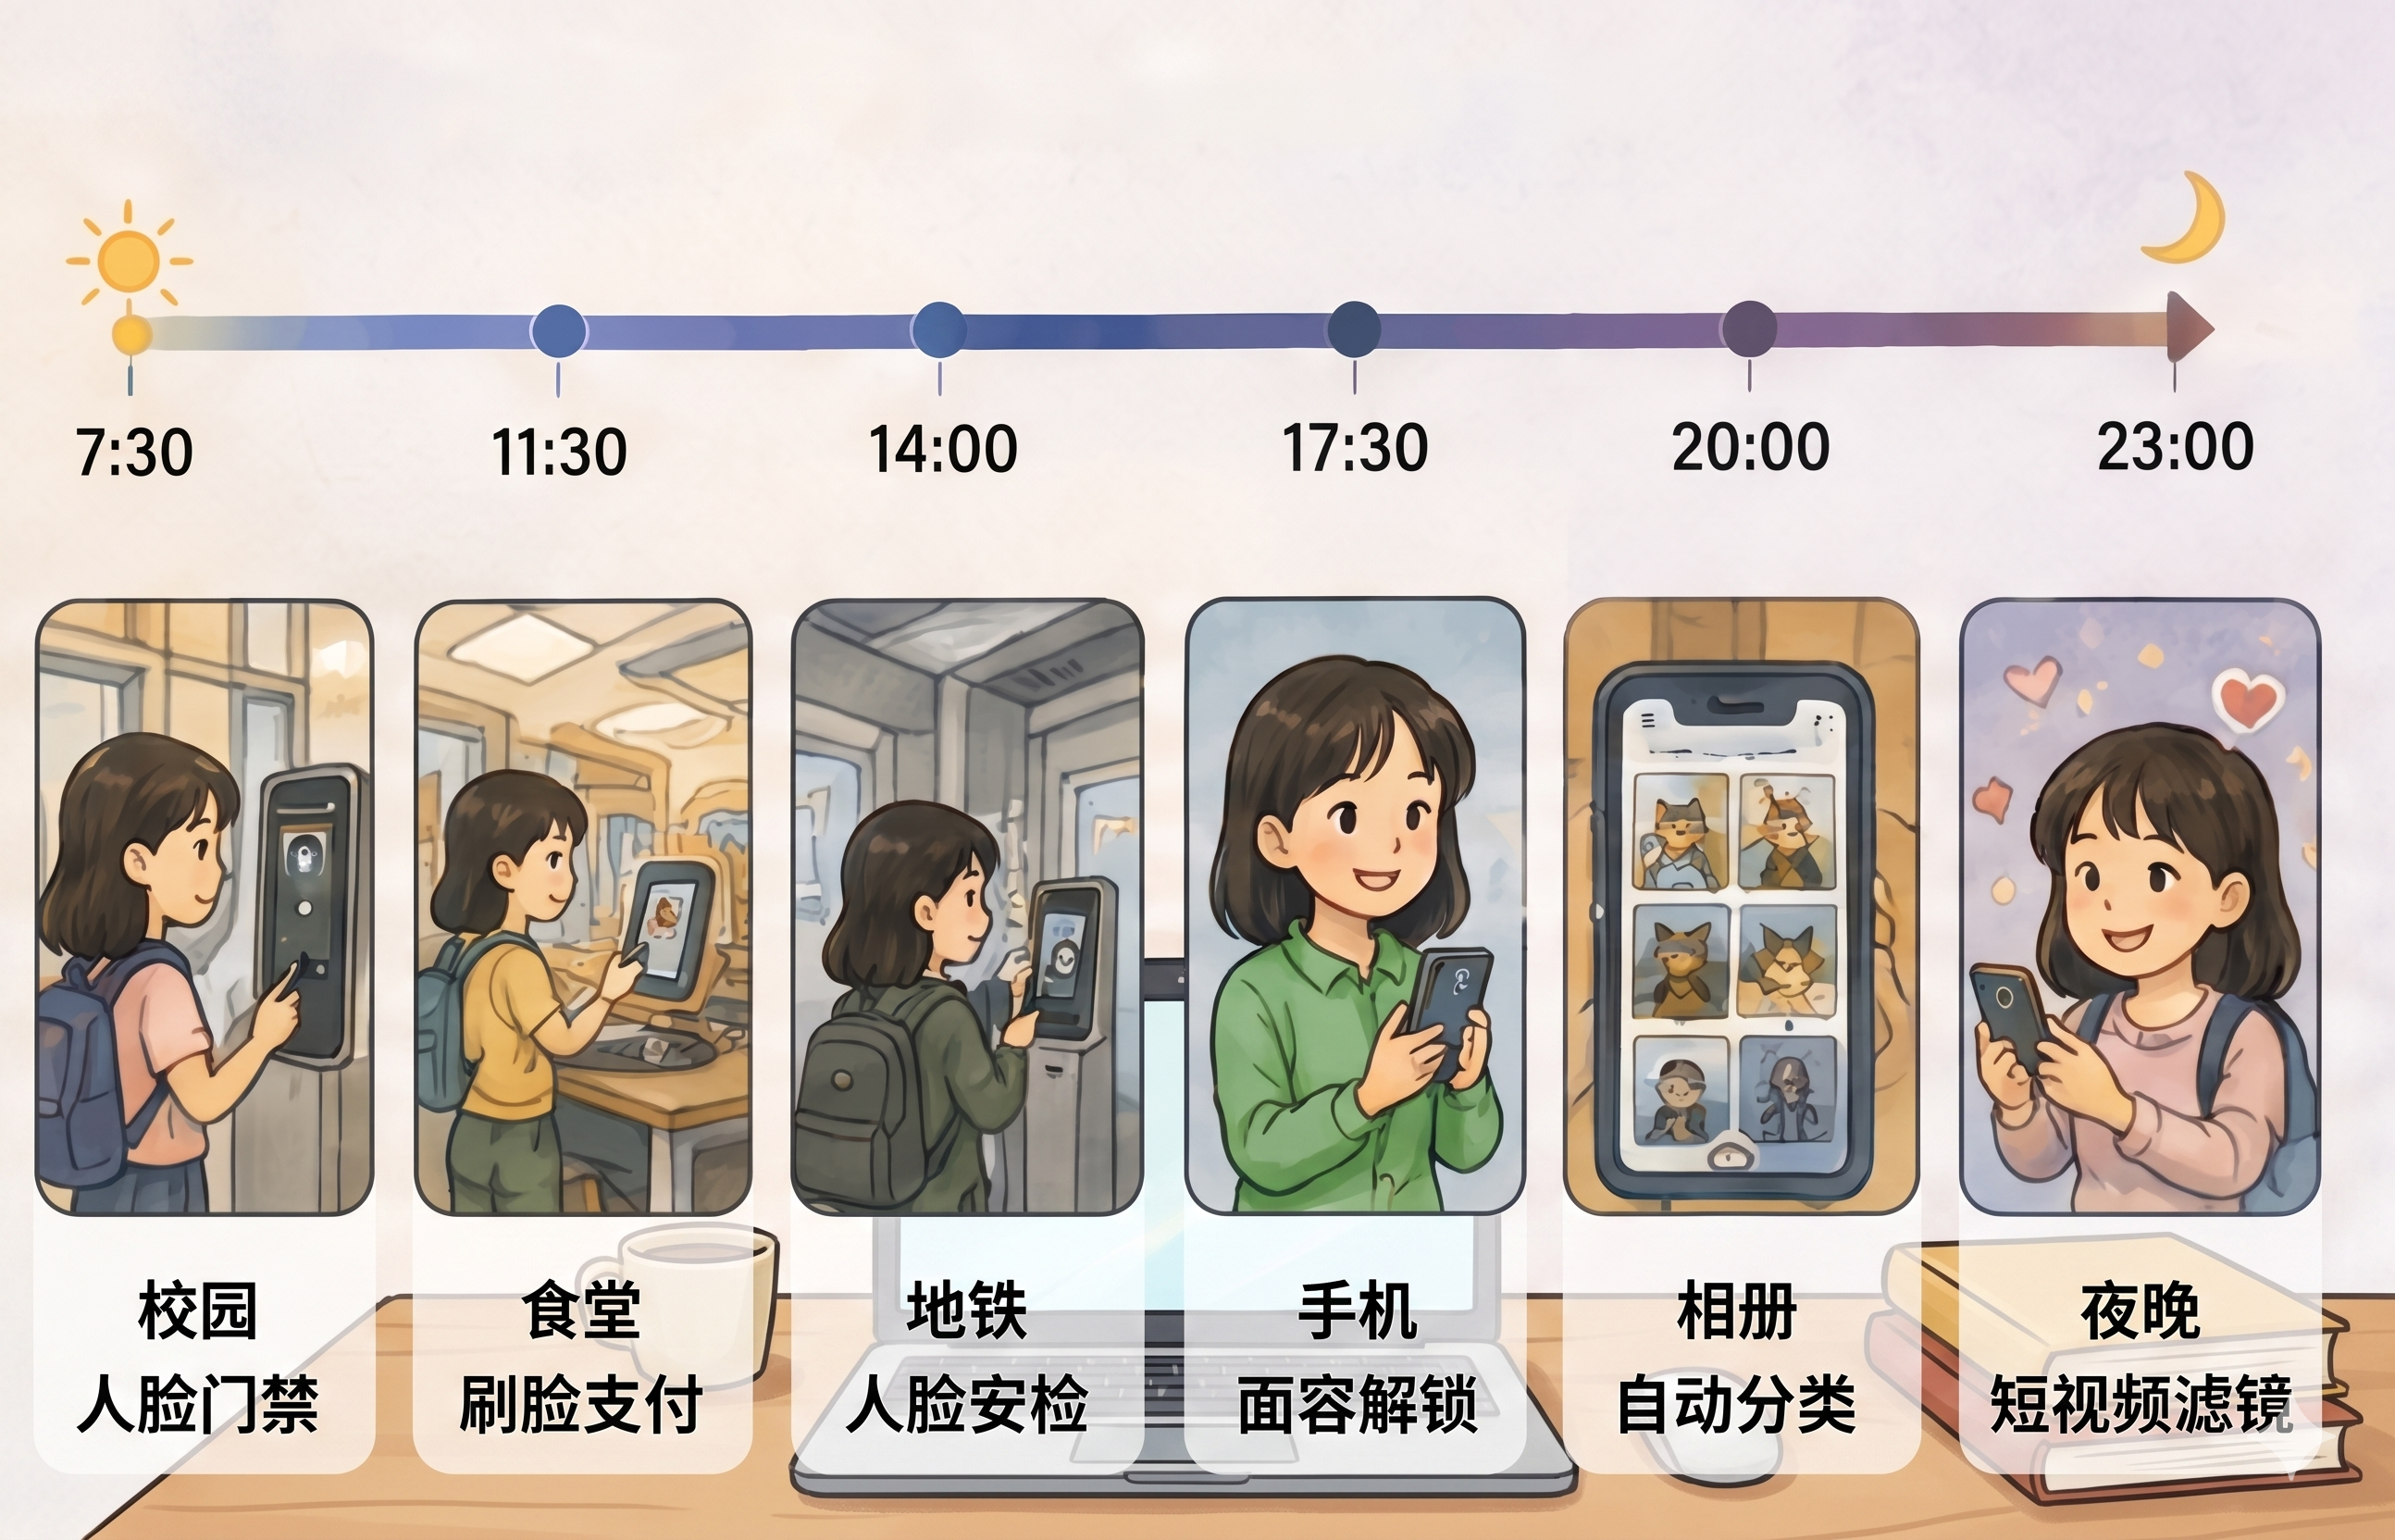
\includegraphics[width=0.88\textwidth]{images_chapter_01-03/2-6.png}
\caption*{\footnotesize\itshape\color{gray!50} 图2-2\quad 推荐系统如何从行为数据中“拼出”用户画像}
\end{figure}

所以，AI到底“创造”了什么？\textbf{AI创造的是“符合人类审美模式的新组合”，而不是“来自真实生命体验的表达”。} 当梵高画《星月夜》时，每一笔扭曲的星空都来自他对世界的独特感知——不是因为他学了一百万张星空画后总结出“星空应该这样画”，而是因为他用那样的方式看世界。AI没有“看世界”的方式。它只是在海量已有作品的基础上，找到了一条“最优重组路径”。

那么，\textbf{AI会取代人类创作者吗？} 答案很可能是：\textbf{AI不会取代人类创作者，但“会用AI的创作者”可能会取代“不会用AI的创作者”。} 就像摄影技术没有取代画家，但永远改变了视觉艺术的方向。AI也是如此。它可能不会“消灭”人类创作，但会改变创作的方式和标准。在AI可以瞬间生成任何风格的图像时，人类画家的价值在哪里？可能在于画出AI生成不出的东西——那些来自真实身体经验、来自具体时空中的独特感知、来自一个有温度的生命对另一个生命的理解。

画笔从毛笔变成钢笔，从钢笔变成数位板。音乐从现场演奏变成录音棚，从黑胶变成流媒体。每一次技术革命，都有人担心“艺术会消亡”。但艺术始终存在，因为人类表达自我的冲动从未消失。AI只是最新的一支“笔”。真正重要的，永远是那个握着笔的人。

\section{AI的能力边界：有所为，有所不为}

走过了机器学习、计算机视觉、自然语言处理和生成式AI四段旅程之后，是时候停下来，把几条线索收拢到一起了。

你会发现一个贯穿始终的共同主题：\textbf{AI在各项能力上展现出的表现都极其强大，但这种强大的本质是“模式识别”和“统计重组”，而不是真正的“理解”和“创造”。}

在本章最后一节，让我们从四个维度来系统讨论AI的边界——它能做什么，绝对不能做什么，以及为什么理解这些“不能”比知道AI“能做什么”更重要。

\subsection{AI为什么会“一本正经地胡说八道”}

2023年春天，大二学生小刘正在赶一篇期末论文。截止时间是第二天中午，他还差三篇参考文献。他灵机一动：让AI直接生成。他输入了详细的提示词：“请推荐5篇关于社交媒体对青少年心理健康影响的近五年学术论文，提供完整的标题、作者、期刊名称和发表年份。”

几秒后，AI返回了五条格式完美的文献——有作者全名，有期刊名称和卷号，有的还附有DOI编号。小刘看都没细看，直接复制粘贴进了论文的参考文献列表。

两天后，老师在课堂上问：“小刘，你这篇论文引用的Smith et al. (2021)，我怎么在期刊数据库里搜不到？”小刘回去一条条核查，发现五篇参考文献里，有三篇完全不存在。作者姓名是真的，期刊也是真期刊，但那些论文从来没有发表过。

\textbf{这就是AI幻觉}——AI生成的内容表达流畅、看似合理，但包含事实性错误或完全虚构的信息。它最危险的地方不是“AI会犯错”——所有工具都会犯错——而是它犯错时看起来和说真话时一样自信。你问它一个它知道正确答案的问题，它语气笃定地回答你。你问它一个它不知道的问题，它同样语气笃定地编造一个。

提示词写得好不好不影响这个问题的存在。因为AI的本质是基于语言规律生成内容，而不是基于事实数据库进行查询。它的目标是“说像人说的话”，不是“说真话”。

所以，\textbf{在任何重要场景中——学业、法律、医疗——AI输出的一切内容，必须经过人工核查。}

\begin{funbox}
\textbf{AI识别坦克的故事——一个关于“伪相关”的经典教训}

在人工智能发展史上，有一个广为流传的经典教训。20世纪80年代，美国军方资助了一个AI项目，目标是让计算机学会自动识别照片中的坦克。研究者收集了大量坦克照片和普通车辆照片作为训练数据，AI在学习后表现出色——在测试集上识别准确率几乎达到100\%。

项目看起来取得了巨大成功。但当系统被部署到实际战场环境中时，它的表现却一落千丈——准确率甚至不如抛硬币。

经过反复排查，研究者发现了一个令人啼笑皆非的问题：训练数据中所有坦克照片都是在阴天拍摄的，而普通车辆照片都是在晴天拍摄的。AI根本没有学会“坦克长什么样”——它只是学会了“阴天=坦克，晴天=普通车辆”。

这个案例完美地说明了AI学习的本质：它不是在“理解”物体是什么，而是在数据中寻找任何能够区分两类样本的统计相关性——无论这个相关性是否真的有意义。这也解释了为什么AI会如此自信地犯错：从统计角度看，“阴天=坦克”和“履带=坦克”一样都是有效的区分规则，AI无法分辨哪个规则是有意义的、哪个是巧合。
\end{funbox}

\subsection{AI也会“戴有色眼镜”}

大二学生阿琳有一段时间特别焦虑。她只是偶然点开了一个健身视频，接下来的几天，整个短视频平台像变了个人：首页全是减肥教程、健身食谱、身材管理经验。甚至有一些视频的标题是“大学女生不管理身材就输了”。

“我只是看了一个健身视频，”阿琳说，“现在它好像觉得我的人生只剩减肥了。”

有人可能会问：这是AI的错吗？从技术上说，AI本身没有“偏见”这个概念。它只是忠实地执行一个指令：\textbf{“推荐用户可能喜欢的内容。”} 但它不知道你点开健身视频是因为假期吃胖了几斤产生的焦虑，它只知道“你点了，我要推更多”。

AI偏见的来源有三个层面：第一，训练数据中的偏见——互联网本身就充满偏见。如果AI学习的招聘数据中CEO大多是男性，AI在筛选简历时就可能更倾向男性。这不是AI“主动歧视”，而是它从数据中学到了“CEO通常是男性”这个统计规律。第二，用户行为造成的偏差——推荐系统会不断强化你已经表现出来的兴趣，让你越看越窄（信息茧房效应）。第三，标签代理偏差——AI常用一些易于测量的特征代替复杂的现实，比如用“点击率”代替“内容质量”，结果就是标题党越来越多。

\textbf{核心认知}：AI并不是绝对客观的。它像一面镜子，反射的是人类社会数据中已经存在的偏见。在很多情况下，AI甚至会放大这些偏见。

\subsection{为什么AI需要人类监督}

2024年，一位独居老人接到电话。“妈，我出事了。”电话那头是儿子的声音。语气急促、恐惧，和平时一模一样。“我开车撞了人，对方家属要赔偿。你先把钱打过来，不要告诉别人，太丢人了。”老人手忙脚乱地翻出存折。就在她准备出门转账时，社区民警入户走访。警察听完描述让她立刻给儿子打个电话确认。电话接通了。儿子正在公司上班，根本没有出车祸。

后来警方调查发现，那通电话不是真人打的。犯罪分子从社交平台上获取了老人儿子的语音数据，使用\textbf{AI语音克隆技术}复制了他的声音。只需要几秒钟的语音样本，AI就能复制一个人的音色、语调、停顿和情绪表达。

\begin{knowledgebox}
\textbf{AI语音克隆与Deepfake——技术的双面刃}

\textbf{AI语音克隆}是指利用AI技术，从几秒钟到几分钟的真人语音样本中提取说话人的音色、语调、停顿和情绪特征，然后生成该说话人从未说过的全新语音内容。其原理类似于生成式AI根据文字描述生成图像——只不过生成的是声音波形。

\textbf{Deepfake}（深度伪造）是“Deep Learning”和“Fake”的合成词，泛指利用深度学习技术伪造视频、音频或图像的技术。换脸视频是最典型、最早引起公众关注的Deepfake应用。Deepfake具有双重属性——既可以用于电影特效、历史人物复原等正当用途，也可能被用于制造虚假新闻和电信诈骗。目前各国正在逐步建立针对Deepfake的法律监管框架。
\end{knowledgebox}

这个故事虽然令人毛骨悚然，但它并不是孤例。随着AI技术越来越强大，滥用AI的门槛也在降低：有人将个人隐私数据上传到不安全的AI平台造成泄露；有人用AI批量生成虚假新闻操纵舆论；Deepfake换脸技术被用来伪造公众人物讲话视频。

请注意：AI本身没有善恶观。它不知道“克隆别人的声音去骗钱”是坏的。它只是一个工具。就像一把刀——可以做一顿美味的晚餐，也可以成为凶器。刀没有善恶，关键在于握刀的人。正因为AI没有道德判断，\textbf{人类监督才必不可少。} 无论AI技术多么先进，最终仍然需要人类制定使用规则、审核产出内容、承担相应责任。

\subsection{AI真正缺少什么}

深夜一点半，大三学生小周睡不着。他刚刚查出期末成绩——专业课考砸了。他不敢告诉父母，不敢告诉同学，一个人窝在被窝里。翻遍通讯录，不知道该找谁说话。犹豫了很久，他打开手机上的AI聊天应用，打了一行字：“我考砸了，很难受。”

AI很快回复：“听到你考砸了，我能理解你现在的心情。一次失败不代表什么，你付出的努力不会白费。”那些话温柔、理性、充满耐心。甚至比一些现实中的人还会安慰人。

小周回了一大段，讲了考试有多难，讲了他复习到凌晨两三点的那些夜晚，讲了看到成绩时手抖的感觉。AI每一条都认真回复。到了凌晨三点，小周打出最后一句：“谢谢你，我感觉好点了。”然后沉沉睡去。

但他没有问自己一个问题：\textbf{“它真的理解我了吗？”}

AI做对了什么？它识别出了“考砸了”和“难过”之间在语言上的关联——因为在训练数据中，这两个词大量共现。它识别出这是一段需要安慰的对话——因为对话的语义模式符合“倾诉-安慰”的场景特征。它能生成符合“温暖、理性、不评判”风格的回复。

但它不能做什么？它不知道“考砸了”对一个具体的人意味着什么。它不会心疼。它没有经历过“努力之后失败”的苦涩——它只是识别出你的文字里有这种情绪的语义表征。它不会在你睡着后还在想“那个学生不知道有没有好起来”。当你关掉对话窗口，这段对话对AI来说就结束了，就像你关掉了一个文档。

\begin{figure}[H]
\centering
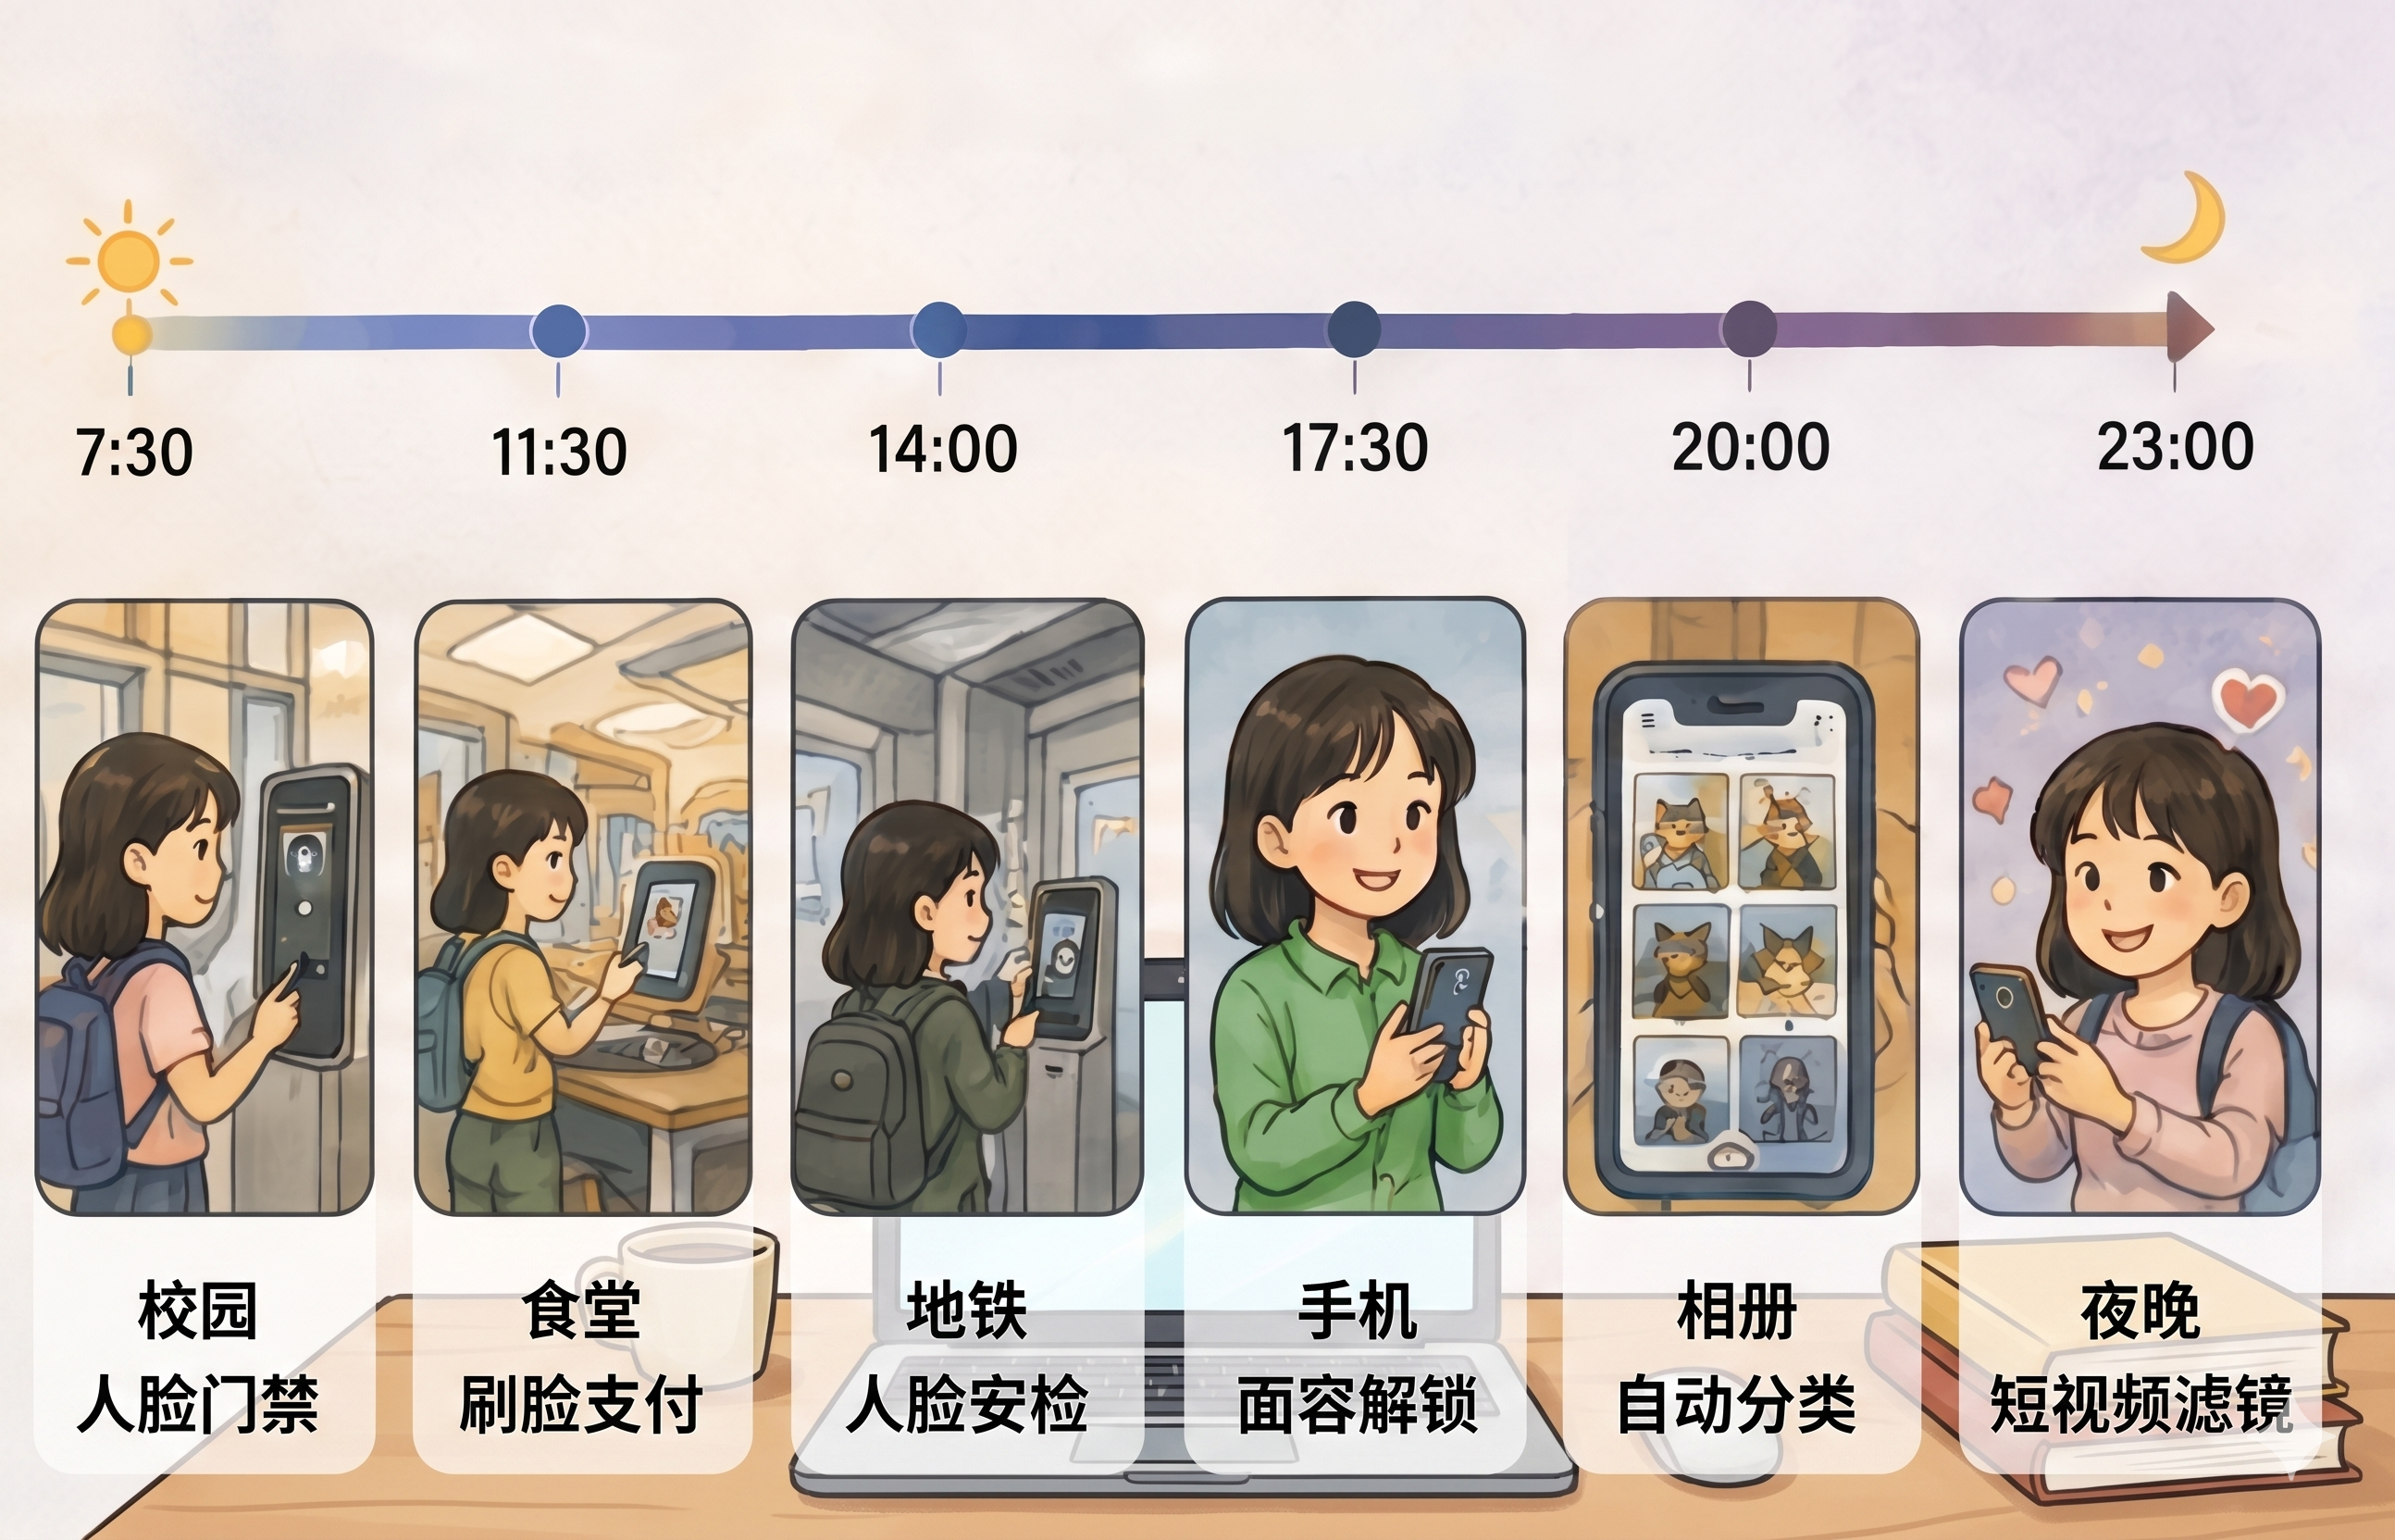
\includegraphics[width=0.88\textwidth]{images_chapter_01-03/2-6.png}
\caption*{\footnotesize\itshape\color{gray!50} 图2-2\quad 推荐系统如何从行为数据中“拼出”用户画像}
\end{figure}

这就是AI最根本的边界。它可以在几秒钟内生成一篇“关于母爱”的感人散文，但它从未有过母亲。它可以模仿一个作家的所有风格特征写出一篇“新作”，但它不知道那位作家在创作时的精神状态。它可以分析大量数据做出商业决策建议，但它无法像人类一样进行道德判断和价值选择。

\textbf{AI不会成为“人”，因为它没有第一人称体验，没有真正的意识和自我觉察，无法进行道德选择和承担后果，没有真实的欲望和意图。} 它只是一面极其强大的镜子——反射人类语言、人类图像、人类创造中的所有模式。但它不是光源本身。

\section*{本章小结}
\addcontentsline{toc}{section}{本章小结}

这一章，我们从四个维度了解了AI如何认识世界。

我们了解了\textbf{机器学习}——AI从数据中总结规律，拦截诈骗短信、预测天气、辅助诊断疾病，但它只是在做概率计算，不是在思考。

我们了解了\textbf{计算机视觉}——AI能从像素中提取特征，识别物体、人脸、路况，但它看到的只是数字和模式，不是意义和情感。

我们了解了\textbf{自然语言处理}——大语言模型让AI变得“能说会道”，但它的语言能力来自海量文本的概率学习，它不理解自己说的话。

我们了解了\textbf{生成式AI}——AI能画画、写文章、做音乐，但它的“创作”本质是模仿重组，而不是真正的灵感迸发。

最后，我们系统地审视了AI的边界：它会一本正经地编造事实，它会忠实复制人类的偏见，它可能被滥用，它永远无法成为有意识、有情感、有道德感的“人”。

\textbf{AI不是魔法，也不是魔鬼。} 它是人类创造的工具——一个极其擅长发现规律、处理信息、生成内容的工具。它的强大在于数据处理的规模和速度，它的局限在于没有意识、没有情感、没有真正的理解能力。

理解了这些，你就拥有了面对AI最重要的东西：\textbf{不是技术能力，而是认知框架。} 你不会把它当神崇拜，也不会把它当鬼恐惧。你会把它当作一个强大的工具——理解它的能力，清楚它的边界，学会和它协作，同时承担作为使用者的判断和责任。

而在理解了AI能做什么、不能做什么之后，一个更实际的问题自然浮现：既然AI是这样工作的，那我们该怎么和它高效协作？怎么写好提示词？怎么让AI从“回答问题”变成“帮你做事”？这就是下一章要回答的问题。
